% !TeX spellcheck = de_DE
\makeglossaries


\newglossaryentry{pseudoinverse}
{name={Pseudoinverse},
  description={Die \textbf{Pseudoinverse}\index{Pseudoinverse} nach Moore–Penrose $\mA^{+}$ 
  	einer \gls{matrix} $\mA \in \mathbb{R}^{\samplesize \times \nrfeatures}$ verallgemeinert das Konzept der 
  	\gls{inverse} \cite{GolubVanLoanBook}. Die Pseudoinverse\cite{unikassel} tritt natürlich im Kontext der 
  	\gls{ridgeregression} auf, wenn diese auf ein \gls{dataset} mit beliebigen \glspl{label} $\vy$ 
  	und einer \gls{featuremtx} $\mX = \mA$ angewendet wird \cite[Kap.\ 3]{hastie01statisticallearning}. 
  	Die durch \gls{ridgeregression} gelernten \glspl{modelparam} ergeben sich zu
  	\[
  	\widehat{\vw}^{(\regparam)}  = \big(\mA\,^{T} \mA + \regparam \mI \big)^{-1} \mA^\top \vy, \quad \regparam > 0.
  	\]
  	Die Pseudoinverse $\mA^+ \in \mathbb{R}^{\nrfeatures \times \samplesize}$ kann dann über den Grenzwert definiert werden \cite[Kap. 3]{benisrael2003generalized}:
  	\[
  	\lim_{\regparam \to 0^+} \widehat{\vw}^{(\regparam)} = \mA^+ \vy.
  	\]
  	\\
  	Siehe auch: \gls{matrix}, \gls{inverse}, \gls{ridgeregression}.
  },
 first={Pseudoinverse},
 text={Pseudoinverse}, 
 plural={Pseudoinverse}
}


\newglossaryentry{randomexperiment}
{name={Zufallsexperiment},
  description={Ein \textbf{Zufallsexperiment}\index{Zufallsexperiment} ist ein physikalischer 
  (oder abstrakter) Prozess, der ein Ergebnis $\omega$ aus einer Ergebnismenge 
  $\Omega$ erzeugt. Diese Menge aller möglichen Ergebnisse wird als 
  \gls{samplespace} des Experiments bezeichnet. Das zentrale Merkmal eines 
  Zufallsexperiments ist, dass dessen Ergebnis unvorhersehbar (oder unsicher) ist. 
  Jede Messung oder Beobachtung des Ergebnisses ist eine \gls{rv}, also eine Funktion 
  des Ergebnisses $\omega \in \Omega$.\\
  Die Wahrscheinlichkeitstheorie verwendet einen \gls{probspace} als mathematische 
  Struktur zur Modellierung von Zufallsexperimenten. Ein wichtiges konzeptuelles 
  Merkmal eines Zufallsexperiments ist, dass es unter identischen Bedingungen 
  wiederholbar ist. Streng genommen definiert die Wiederholung eines 
  Zufallsexperiments $\samplesize$-mal ein neues Zufallsexperiment. Die Ergebnisse 
  dieses neuen Experiments sind Folgen der Länge $\samplesize$ bestehend aus den 
  Einzelergebnissen des ursprünglichen Experiments. Während das Ergebnis eines 
  einzelnen Experiments zufällig ist, wird das Langzeitverhalten wiederholter 
  Experimente zunehmend vorhersagbar. Diese informelle Aussage wird durch 
  grundlegende Resultate der \gls{probability} wie das \gls{lln} und das \gls{clt} 
  mathematisch präzisiert. 
  \begin{figure}[h]
	\begin{center}
	 \begin{tikzpicture}[>=Stealth, node distance=1.5cm and 2cm, every node/.style={font=\small}]
		\node (experiment) [draw, rectangle, rounded corners, minimum width=2.6cm, align=center] {Zufallsexperiment};
		\node (omega) [right=of experiment] {$\omega \in \Omega$};
		\coordinate (rightpad) at ($(omega.east) + (0.2,0)$);
		\draw[->] (experiment) -- (omega);
		\node (sequence) [below=of experiment, yshift=-0.5cm] {$(\omega^{(1)}, \omega^{(2)}, \dots, \omega^{(\samplesize)})$};
		\node (sequence1) [below=of sequence, yshift=-0.5cm] {$(\datapoint^{(1)}, \datapoint^{(2)}, \dots, \datapoint^{(\samplesize)})$};
		\draw[->, thick] (experiment.south) -- node[midway, right, xshift=3pt] {Wiederholung $\samplesize$-mal} (sequence.north);
		\draw[->, thick] (sequence.south) -- node[midway, right, xshift=3pt] {\glspl{rv}} (sequence1.north);
		\path (experiment.south) -- (sequence.north) coordinate[pos=0.6] (repeatpoint);
        \node[draw=black, rounded corners, dotted, fit={(experiment) (repeatpoint) (rightpad)}, inner sep=8pt, label=above:{neues Zufallsexperiment mit $\Omega' = \Omega \times \ldots \times \Omega$}] {};
	 \end{tikzpicture}
	\end{center}
	\caption{Ein Zufallsexperiment erzeugt ein Ergebnis $\omega \in \Omega$ aus einer Ergebnismenge (oder \gls{samplespace}) $\Omega$. Die Wiederholung des Experiments $\samplesize$-mal ergibt ein neues Zufallsexperiment, dessen Ergebnisse Folgen $(\omega^{(1)}, \omega^{(2)}, \dots, \omega^{(\samplesize)}) \in \Omega\times\ldots\times \Omega$ sind. Ein Beispiel für ein Zufallsexperiment in \gls{ml}-Anwendungen ist die Erhebung eines \gls{trainset} $\datapoint^{(1)},\ldots,\datapoint^{(\samplesize)}$.}
  \end{figure}
  Beispiele für Zufallsexperimente in \gls{ml}-Anwendungen sind:
  \begin{itemize}
  	\item \Gls{data}-Erhebung: Die im Rahmen von \gls{erm}-basierten Methoden erhobenen \glspl{datapoint} können als \glspl{rv}, d.\,h. als Funktionen des Zufallsergebnisses $\omega \in \Omega$ interpretiert werden.
  	\item \Gls{stochGD} nutzt in jeder Iteration ein Zufallsexperiment, um eine Teilmenge des \gls{trainset} auszuwählen.
  	\item \Gls{privprot}-Methoden verwenden Zufallsexperimente zur Generierung von Rauschen, das den Ausgaben eines \gls{ml}-Verfahrens hinzugefügt wird, um \gls{diffpriv} zu gewährleisten.
  \end{itemize}},
firstplural={Zufallsexperimente},
plural={Zufallsexperimente},
first={Zufallsexperiment},
text={Zufallsexperiment}, 
plural={Zufallsexperimente}
}

\newglossaryentry{dimension}

{name={Dimension},
 description={
 Die \index{Dimension}Dimension \(\dim \mathcal{A}\) eines \gls{vectorspace}es \(\mathcal{A}\) ist die Mächtigkeit (Kardinalität) einer beliebigen \gls{basis} von \(\mathcal{A}\) \cite{Axler2025}. 
 Streng genommen gilt diese Definition nur für endlich-dimensionale \glspl{vectorspace}, d. h., solche, die eine endliche \gls{basis} besitzen. 
 \begin{figure}[H]
  \begin{tikzpicture}[scale=1]
   \coordinate (O) at (0,0);
   % Basis 1: Standard (durchgezogen)
   \draw[->, thick] (O) -- (1.8,0) node[below right] {\(\ve^{(1)}\)};
   \draw[->, thick] (O) -- (0,1.6) node[above left] {\(\ve^{(2)}\)};
   % Basis 2: um ca. 45° gedreht (gestrichelt)
   \draw[->, thick, dashed, shift={(3.5,0.5)}] (0,0) -- (1.2,1.2) node[above right] {\(\vu^{(1)}\)};
   \draw[->, thick, dashed, shift={(3.5,0.5)}] (0,0) -- (-1.2,1.2) node[above left] {\(\vu^{(2)}\)};
   % Basis 3: nicht orthogonal / schief (gepunktet)
   \draw[->, thick, dotted, shift={(-2.5,-2.5)}] (0,0) -- (2.0,0.6) node[above right] {\(\vw^{(1)}\)};
   \draw[->, thick, dotted, shift={(-2.5,-2.5)}] (0,0) -- (0.4,1.8) node[left] {\(\vw^{(2)}\)};
  \end{tikzpicture}
  \caption{Drei \glspl{basis}, \(\{\ve^{(1)},\ve^{(2)}\}, \{\vu^{(1)},\vu^{(2)}\}, \{\vw^{(1)},\vw^{(2)}\}\) für den \gls{vectorspace} \(\mathbb R^2\).}
 \end{figure}
 Für solche Räume haben alle \glspl{basis} dieselbe Mächtigkeit, welche dann die Dimension\citation{Thomas2013LineareAlgebra} des Raumes ist \cite[Kap. 2]{Axler2025}.\\
 Siehe auch: \gls{vectorspace}, \gls{basis}.
 },
 text = {Dimension},
 first = {Dimension},
 plural= {Dimensionen},
}

\newglossaryentry{linearlyindep}
{name={linear unabhängig},
 description={
 Eine Teilmenge $\{\va^{(1)}, \,\ldots, \,\va^{(\nrfeatures)}\} \subset \mathcal{V}$ 
 eines \gls{vectorspace}es heißt \emph{linear unabhängig}\index{linear unabhängig}\cite{Thomas2013LineareAlgebra}{,p.90}, 
 wenn keine nichttriviale Linearkombination dieser \glspl{vector} 
 den Null\gls{vector} ergibt \cite{StrangLinAlg2016}. 
 Anders ausgedrückt gilt:
 \[
 \sum_{\featureidx=1}^{\nrfeatures} \alpha_{\featureidx} \va^{(\featureidx)} = \mathbf{0}	
 \quad \text{impliziert} \quad \alpha_{1} = \alpha_{2} = \ldots = \alpha_{k} = 0.
 \]
 \\[0.5em]
 Siehe auch: \gls{vectorspace}, \gls{vector}, \gls{dimension}, \gls{basis}.
 },
 text = {linear unabhängig},
 first = {linear unabhängig},
 plural= {linear unabhängige}
}


\newglossaryentry{basis}
{
  name={Basis},
  description={Eine Basis\index{Basis}\cite{Soergel201x_AlgebraMitBildern} eines \gls{Vektorraums} $\mathcal{V}$ 
  ist eine Menge von \glspl{linearunabhaengig}en \glspl{Vektor}en 
  $\{\va^{(1)}, \,\ldots, \,\va^{(\nrfeatures)}\}$, 
  sodass jeder Vektor $\va \in \mathcal{V}$ als Linearkombination 
  der Basisvektoren dargestellt werden kann, d.\,h.
  $$
    \va = \sum_{\featureidx=1}^{\nrfeatures} \alpha_{\featureidx} \va^{(\featureidx)} 
    \quad \text{für gewisse } \alpha_{1}, \,\ldots, \,\alpha_{\nrfeatures} \in \mathbb{R}.
  $$
  },
  text = {Basis}, 
  firstplural={Basen}, 
  plural={Basen}, 
  type=math,
  first = {Basis}
}


\newglossaryentry{widematrix}
{
  name={breite Matrix},
  description={Eine\index{breite Matrix} \gls{Matrix} 
  $\mA \in \mathbb{R}^{\samplesize \times \nrfeatures}$ 
  wird als \emph{breit} bezeichnet, wenn sie mehr Spalten als Zeilen besitzt, 
  d.\,h. $\nrfeatures > \samplesize$.\\ 
  Siehe auch: \gls{Matrix}.},
  text = {breite Matrix}, 
  firstplural={Breite Matrizen}, 
  plural={breite Matrizen}, 
  type=math,
  first = {breite Matrix}
}

\newglossaryentry{tallmatrix}
{
  name={hohe Matrix},
  description={Eine\index{hohe Matrix} \gls{Matrix} 
  $\mA \in \mathbb{R}^{\samplesize \times \nrfeatures}$ 
  wird als \emph{hoch} bezeichnet, wenn sie mehr Zeilen als Spalten besitzt, 
  d.\,h. wenn $\samplesize > \nrfeatures$.\\ 
  Siehe auch: \gls{Matrix}.},
  text = {hohe Matrix}, 
  firstplural={Hohe Matrizen}, 
  plural={hohe Matrizen}, 
  type=math,
  first = {hohe Matrix}
}


\newglossaryentry{rankdeficient}
{
  name={rangdefizient},
  description={Eine \gls{Matrix} $\mA \in \mathbb{R}^{\samplesize \times \nrfeatures}$ 
   ist \index{rangdefizient} rangdefizient\cite{Krause2021}, wenn sie nicht vollen Rang besitzt, 
  d.\,h. wenn $\rank{\mA} < \min\{\samplesize, \nrfeatures\}$ gilt.\\
  Siehe auch: \gls{vollerang}. 
  }, 
  first={rangdefizient}, 
  text={rangdefizient}
  plural= 
}

\newglossaryentry{fullrank}
{
  name={voller Rang},
  description={Eine \gls{Matrix} $\mA \in \mathbb{R}^{\samplesize \times \nrfeatures}$ 
  ist \index{voller Rang} voller Rang, wenn sie den maximalen \gls{Rang} besitzt \cite{StrangLinAlg2016}. 
  Für eine hohe \gls{Matrix}, d.\,h. wenn $\nrfeatures < \samplesize$, bedeutet voller Rang, dass ihr \gls{Rang} gleich $\nrfeatures$ ist. 
 \begin{figure}[H]
\centering
\begin{tikzpicture}[every node/.style={font=\small}]
% --- Full-rank square ---
\node at (0,2) {$
\mA =
\begin{pmatrix}
1 & 2\\
3 & 4
\end{pmatrix}
$};
\node[below=0.8cm of {$(0,2)$}] {\small voller Rang, quadratisch};
% --- Rank-deficient square ---
\node at (4.5,2) {$
\mB =
\begin{pmatrix}
1 & 2\\
2 & 4
\end{pmatrix}
$};
\node[below=0.8cm of {$(4.5,2)$}] {\small \gls{rankdeficient}, quadratisch};
% --- Full-rank tall (3x2) ---
\node at (0,-1.0) {$
\mC =
\begin{pmatrix}
1 & 0\\
0 & 1\\
1 & 1
\end{pmatrix}
$};
\node[below=1.2cm of {$(0,-1.0)$}] {\small voller Rang, \gls{tallmatrix}};
% --- Rank-deficient wide (2x3) ---
\node at (4.5,-1.0) {$
\mD =
\begin{pmatrix}
1 & 2 & 3\\
2 & 4 & 6
\end{pmatrix}
$};
\node[below=1.2cm of {$(4.5,-1.0)$}] {\small \gls{rankdeficient}, \gls{widematrix}};
\end{tikzpicture}
\caption{Beispiele für \glspl{matrix} mit vollem Rang und \gls{rankdeficient}.}
\end{figure} 
  Eine quadratische Matrix ist genau dann voller Rang, wenn sie invertierbar ist.\\
  Siehe auch: \gls{matrix}, \gls{dimension}, \gls{linearmap}, \gls{columnspace}.}, 
  text = {voller Rang}, 
  type=math,
  first = {voller Rang},
  plural={volle Ränge}
}

\newglossaryentry{rank}
{
  name={Rang},
  description={Der Rang\index{Rang} einer \gls{matrix} $\mA \in \mathbb{R}^{\samplesize \times \nrfeatures}$, 
  bezeichnet als $\rank{\mA}$, ist die maximale Anzahl linear unabhängiger Spalten von $\mA$ \cite{StrangLinAlg2016}. 
  Äquivalent kann der Rang auch als die \gls{dimension} des \gls{columnspace} 
  $\linspan{\mA} = \big\{ \mA \weights \mbox{ für ein } \weights \in \mathbb{R}^{\nrfeatures} \big\}$ definiert werden. 
  Der Rang einer \gls{matrix} $\mA \in \mathbb{R}^{\samplesize \times \nrfeatures}$ 
  kann weder die Anzahl der Zeilen noch die Anzahl der Spalten von $\mA$ überschreiten \cite{Horn91,MeyerMatrixAnalysis}, 
  d.h., $\rank{\mA} \leq \min \{ \samplesize, \nrfeatures \}$. \\
  Siehe auch: \gls{matrix}, \gls{dimension}, \gls{linearmap}, \gls{columnspace}.},
  text={Rang},
  type=math,
  first={Rang},
  plural= {Ränge}
}



\newglossaryentry{inverse}
{name={inverse Matrix},
 description={Eine \textbf{inverse \gls{matrix}}\index{inverse Matrix} $\mA^{-1}$ ist für eine 
 	quadratische \gls{matrix} $\mA \in \mathbb{R}^{n \times n}$ definiert, sofern diese vollen Rang besitzt, 
 	d.\,h. ihre Spalten sind linear unabhängig. In diesem Fall heißt $\mA$ \emph{invertierbar} 
 	und ihre Inverse erfüllt
 	\[
 	\mA \mA^{-1} = \mA^{-1} \mA = \mI.
 	\]
 	Eine quadratische \gls{matrix} ist genau dann invertierbar, wenn ihre \gls{det} ungleich null ist.
 	Inverse \glspl{matrix} sind grundlegend beim Lösen von linearen Gleichungssystemen sowie in 
 	der geschlossenen Lösung der \gls{linreg} \cite{Strang2007}, \cite{Horn91}.\\
 	Das Konzept der inversen \gls{matrix} lässt sich auf nicht-quadratische oder singuläre 
 	\glspl{matrix} erweitern. Man kann beispielsweise eine \emph{linksinverse} $\mB$ mit 
 	$\mB \mA = \mI$ oder eine \emph{rechtsinverse} $\mC$ mit $\mA \mC = \mI$ definieren.
 	Für allgemeine rechteckige oder singuläre \glspl{matrix} liefert die Moore–Penrose-\gls{pseudoinverse} 
 	$\mA^{+}$ ein einheitliches Konzept der \emph{verallgemeinerten Inversen} \gls{matrix} 
 	\cite{GolubVanLoanBook}.
 	\begin{figure}[H]
 		\centering
 		\begin{tikzpicture}[x=2cm,y=2cm]
 			% LINKS: Standardbasis
 			\begin{scope}
 				\draw[->, thick] (0,0) -- (1,0) node[below right] {$\vx$};
 				\draw[->, thick] (0,0) -- (0,1) node[above left] {$\vy$};
 			\end{scope}
 			% MITTE: Transformation durch A
 			\begin{scope}[shift={(2.0,0)}]
 				\coordinate (A) at (1.5,0.5);
 				\coordinate (B) at (-0.2,1.2);
				\draw[->, very thick, red] (0,0) -- (A) node[pos=0.5, below right] {$\mA \vx$};
 				\draw[->, very thick, red] (0,0) -- (B) node[above right] {$\mA \vy$};
 			\end{scope}
 			% RECHTS: Inverse Transformation
 			\begin{scope}[shift={(4.9,0)}]
 				\draw[->, very thick, blue] (0,0) -- (1,0) node[pos=0.5, below] {$\mA^{-1} (\mA \vx) = \vx$};
 				\draw[->, very thick, blue] (0,0) -- (0,1) node[above] {$\mA^{-1} (\mA \vy) = \vy$};
 			\end{scope}
 			%  Pfeile
 			\draw[->, thick, bend left=20] (1.2,0.4) to node[above] {$\mA$} (1.8,0.4);
 			\draw[->, thick, bend left=20] (3.8,0.4) to node[below] {$\mA^{-1}$} (4.4,0.4);
 		\end{tikzpicture}
 		\caption{Eine \gls{matrix} $\mathbf{A}$ beschreibt eine lineare Transformation des $\mathbb{R}^{2}$. 
 		Die inverse \gls{matrix} $\mathbf{A}^{-1}$ beschreibt die Umkehrtransformation. 
 		\label{fig_matrix_inverse_dict}} 
 	\end{figure}
 	Siehe auch: \gls{matrix}, \gls{det}, \gls{linreg}, \gls{pseudoinverse}.},
first={inverse Matrix},
text={inverse Matrix}
}

\newglossaryentry{matrix}
{
  name={Matrix},
  description={Eine Matrix\index{Matrix} der Größe $\samplesize \times \nrfeatures$ ist ein zweidimensionales Zahlenarray, 
    das wie folgt dargestellt wird:
    $$
    \mA = \begin{pmatrix}
      A_{1,1} & A_{1,2} & \dots  & A_{1,\nrfeatures} \\
      A_{2,1} & A_{2,2} & \dots  & A_{2,\nrfeatures} \\
      \vdots  & \vdots  & \ddots & \vdots \\
      A_{\samplesize,1} & A_{\samplesize,2} & \dots  & A_{\samplesize,\nrfeatures}
    \end{pmatrix} \in \mathbb{R}^{\samplesize \times \nrfeatures}.
    $$
    Dabei bezeichnet $A_{\sampleidx,\featureidx}$ den Eintrag der Matrix in der $\sampleidx$-ten Zeile 
    und der $\featureidx$-ten Spalte. Matrizen sind nützliche Darstellungen verschiedener mathematischer Objekte \cite{StrangLinAlg2016}, 
    darunter:
    \begin{itemize}
      \item Systeme linearer Gleichungen: Eine Matrix kann ein System linearer Gleichungen darstellen:
      $$
      \begin{pmatrix}
        A_{1,1} & A_{1,2} \\
        A_{2,1} & A_{2,2}
      \end{pmatrix}
      \begin{pmatrix}
        w_1 \\
        w_2
      \end{pmatrix}
      =
      \begin{pmatrix}
        y_1 \\
        y_2
      \end{pmatrix}
      \quad \text{kompakt geschrieben als } \quad \mA \vw = \vy.
      $$
      Ein wichtiges Beispiel hierfür ist die Optimalitätsbedingung für die 
      \glspl{modelparam} innerhalb der \gls{linreg}.
      \item \Glspl{linearmap}: 
      Betrachte einen $\nrfeatures$-dimensionalen \gls{vectorspace} $\mathcal{U}$ und einen $\samplesize$-dimensionalen \gls{vectorspace} $\mathcal{V}$. 
      Wenn wir eine Basis $\mathbf{u}^{(1)},\,\ldots,\,\mathbf{u}^{(\nrfeatures)}$ für $\mathcal{U}$ und eine Basis 
      $\mathbf{v}^{(1)},\,\ldots,\,\mathbf{v}^{(\samplesize)}$ für $\mathcal{V}$ festlegen, definiert jede Matrix 
      $\mA \in \mathbb{R}^{\samplesize \times \nrfeatures}$ auf natürliche Weise eine 
      \gls{linearmap} $\alpha: \mathcal{U} \rightarrow \mathcal{V}$ (siehe Abb. \ref{fig_matrix_dict}) so, dass
      $$\vu^{(\featureidx)} \mapsto \sum_{\sampleidx=1}^{\samplesize} A_{\sampleidx,\featureidx} \vv^{(\sampleidx)}.$$
      \item \Glspl{dataset}: Eine Matrix kann zur Darstellung eines \gls{dataset} verwendet werden. Jede Zeile 
      entspricht einem einzelnen \gls{datapoint}, jede Spalte einer bestimmten \gls{feature} oder \gls{label} eines \gls{datapoint}.
    \end{itemize}
    \begin{figure}[H]
    \begin{center}
    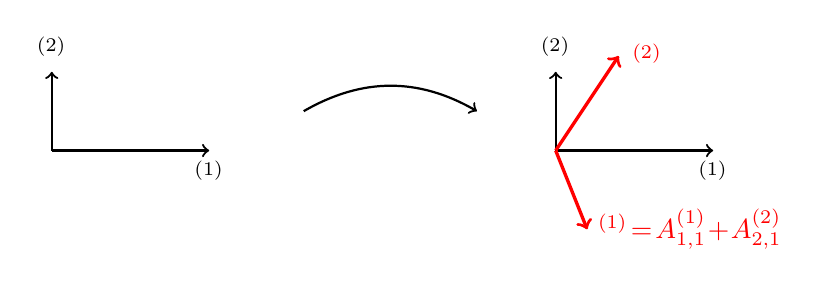
\begin{tikzpicture}[x=2cm]
      % LEFT: Standard basis vectors and unit square
      \begin{scope}
        \draw[->, thick] (0,0) -- (1,0) node[below] {$\vu^{(1)}$};
        \draw[->, thick] (0,0) -- (0,1) node[above] {$\vu^{(2)}$};
      \end{scope}
      % RIGHT: Transformed basis vectors and parallelogram
      \begin{scope}[shift={(3.2,0)}]
        \draw[->, thick] (0,0) -- (1,0) node[below] {$\vv^{(1)}$};
        \draw[->, thick] (0,0) -- (0,1) node[above] {$\vv^{(2)}$};
        \coordinate (A) at (0.2,-1.0);
        \coordinate (B) at (0.4,1.2);
        \draw[->, very thick, red] (0,0) -- (A) node[below,right] {$\mA \vu^{(1)}\!=\!A_{1,1}\vv^{(1)}\!+\!A_{2,1}\vv^{(2)}$};
        \draw[->, very thick, red] (0,0) -- (B) node[right,xshift=1pt] {$\mA \vu^{(2)}$};
      \end{scope}
      % Arrow between plots
      \draw[->, thick] (1.6,0.5) to[bend left] node[midway, above] {$\mA$} (2.7,0.5);
    \end{tikzpicture}
    \end{center}
    \caption{Eine Matrix $\mA$ definiert eine \gls{linearmap} zwischen zwei \glspl{vectorspace}. \label{fig_matrix_dict}} 
    \end{figure}
    Siehe auch: \gls{linearmap}, \gls{dataset}, \gls{linmodel}.},
  first={Matrix},
  firstplural={Matrizen},
  type=math,
  plural={Matrizen},
  text={Matrix}
}

\newglossaryentry{stratification}
{
  name={Stratifizierung},
  description={Stratifizierung bezeichnet den Prozess, ein \gls{dataset} in Teilmengen zu unterteilen, die als \glspl{stratum} bezeichnet werden, 
  entsprechend einem bestimmten Schlüsselkriterium \cite{oecd2008glossary,Everitt2010,OxfordStatisticsDictionary}.
Ziel dieses Vorgehens ist es sicherzustellen, dass eine \gls{ml}-Methode für jedes durch diese Attribute 
 definierte \gls{stratum} gute Leistungen erbringt. In einem medizinischen \gls{dataset} kann es zum Beispiel sinnvoll sein, 
 Patienten nach Altersgruppen zu stratifizieren, um die Leistungsfähigkeit eines \gls{ml}-Modells über alle Altersgruppen hinweg zu gewährleisten.  

  \begin{figure}[H]
  	\centering
	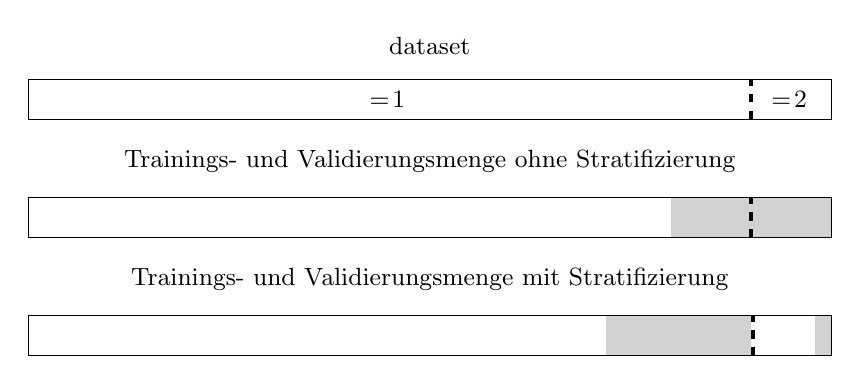
\begin{tikzpicture}[font=\small,x=1.7cm]
		\def\cellw{6.0}
		\def\cellh{0.5}
		\def\gap{1}
		\def\tfrac{0.8}
		\def\pA{0.9}
		\node[anchor=south] at (0.5*\cellw, \cellh+0.2) {\gls{dataset}};
		\node[anchor=south] at ({0.5*\cellw}, {-(\cellh+\gap)+\cellh+0.2}) {Trainings- und Validierungsmenge ohne Stratifizierung};
		\node[anchor=south] at (0.5*\cellw, {-2*(\cellh+\gap)+\cellh+0.2}) {Trainings- und Validierungsmenge mit Stratifizierung};
		\pgfmathsetmacro{\yDataset}{0}
		\pgfmathsetmacro{\yNoStrat}{-(\cellh+\gap)}
		\pgfmathsetmacro{\yStrat}{-2*(\cellh+\gap)}
		\pgfmathsetmacro{\xAB}{\pA*\cellw}
		\pgfmathsetmacro{\wA}{\pA*\cellw}
		\pgfmathsetmacro{\wB}{(1-\pA)*\cellw}
		\draw (0,\yDataset) rectangle ++(\cellw,\cellh);
		\draw[dashed,  line width=0.5mm] (\xAB,\yDataset) -- ++(0,\cellh);
		\node at (0.5*\wA, \yDataset+0.5*\cellh) {$\sensattr\!=\!1$};
		\node at ({\xAB+0.5*\wB}, {\yDataset+0.5*\cellh}) {$\sensattr\!=\!2$};
		\draw (0,\yNoStrat) rectangle ++(\cellw,\cellh);
		\pgfmathsetmacro{\xValStart}{\tfrac*\cellw}
		\pgfmathsetmacro{\valw}{(1-\tfrac)*\cellw}
		\fill[gray!35] (\xValStart,\yNoStrat) rectangle ++(\valw,\cellh);
		\draw[dashed,  line width=0.5mm] (\xAB,\yNoStrat) -- ++(0,\cellh);
		\draw (0,\yStrat) rectangle ++(\cellw,\cellh);
		\pgfmathsetmacro{\xAB}{\pA*\cellw}
		\draw[dashed, line width=1mm] (\xAB,\yStrat) -- ++(0,\cellh);
		\pgfmathsetmacro{\xAVal}{\tfrac*\wA}
		\pgfmathsetmacro{\wAVal}{(1-\tfrac)*\wA}
		\fill[gray!35] (\xAVal,\yStrat) rectangle ++(\wAVal,\cellh);
		\pgfmathsetmacro{\xBVal}{\xAB + \tfrac*\wB}
		\pgfmathsetmacro{\wBVal}{(1-\tfrac)*\wB}
		\fill[gray!35] (\xBVal,\yStrat) rectangle ++(\wBVal,\cellh);
	\end{tikzpicture}
  	\caption{Stratifizierung stellt sicher, dass sowohl die \gls{trainset} als auch die \gls{valset} ähnliche Verteilungen eines binären Schlüsselattributs $\sensattr$ aufweisen.}
  \end{figure}
  
  Wenn ein \gls{dataset} in eine \gls{trainset} und eine \gls{valset} aufgeteilt wird, sorgt die Stratifizierung dafür, dass beide Mengen
ähnliche Verteilungen des Schlüsselattributs enthalten. Ohne Stratifizierung kann eine kleine \gls{valset} die \glspl{datapoint} mit seltenen
 Attributen unterrepräsentieren oder vollständig ausschließen. Dies kann zu irreführenden Leistungsschätzungen führen.\\
  
  Siehe auch: \gls{validation}, \gls{kfoldcv}, \gls{stratum}.},
  text={Stratifizierung},
  first={Stratifizierung},
  plural={Stratifizierungen}
}

\newglossaryentry{stratum}
{
  name={Stratum},
  description={
Ein \index{Stratum} Stratum ist eine Teilmenge von \glspl{datapoint}, die alle eine gemeinsame Eigenschaft besitzen. Diese Eigenschaft kann entweder ein \gls{feature} oder ein \gls{label} sein. Zum Beispiel bilden in einem Wetter-\gls{dataset} alle Messungen von derselben \gls{fmi}-Wetterstation ein Stratum.\\[0.5em]
\begin{center}
\textbf{Beispiel (CSV-Ausschnitt):}\\
{\ttfamily
time,station,value,units\\
2023-06-01 12:00,Helsinki,18.2,degC\\
2023-06-01 13:00,Helsinki,18.5,degC\\
2023-06-01 14:00,Helsinki,19.0,degC\\
2023-06-01 12:00,Oulu,12.1,degC\\
2023-06-01 13:00,Oulu,12.4,degC\\
2023-06-01 14:00,Oulu,12.7,degC\\
2023-06-01 12:00,Tampere,15.3,degC\\
2023-06-01 13:00,Tampere,15.6,degC\\
2023-06-01 14:00,Tampere,16.0,degC
}
\end{center} 
Die Zeilen für jede Wetterstation (\texttt{Helsinki}, \texttt{Oulu}, \texttt{Tampere}) repräsentieren verschiedene Strata.\\
Siehe auch: \gls{stratification}, \gls{dataset}, \gls{datapoint}.},
  first={Stratum},
  firstplural={Strata},
  plural={Strata},
  text={Stratum}
}



\newglossaryentry{det}
{name={Determinante},
 description={Die \textbf{Determinante}\index{Determinante} $\det\,(\mA)$ einer quadratischen \gls{matrix} 
	$\mA = \big( \va^{(1)},\ldots, \va^{(\nrfeatures)} \big) \in \mathbb{R}^{\nrfeatures \times \nrfeatures}$ 
	ist eine \gls{funktion} ihrer Spaltenvektoren $\va^{(1)},\ldots,\va^{(\nrfeatures)} \in \mathbb{R}^{\nrfeatures}$ 
	\cite{DirschmidHansJorg1996TuF} mit folgenden Eigenschaften:
	\begin{itemize}
		\item \textbf{Normiert:} $$\det (\mI) = 1$$
		\item \textbf{Multilinear:}
		\begin{align} \nonumber
		\det \big(\va^{(1)},\ldots,\alpha\vu+ \beta \vv,\ldots,\va^{(\nrfeatures)} \big)
		&= \alpha\det \big(\va^{(1)},\ldots,\vu,\ldots,\va^{(\nrfeatures)} \big) \\
		&+ \beta\det \big(\va^{(1)},\ldots,\vv,\ldots,\va^{(\nrfeatures)} \big) \nonumber
		\end{align}
		\item \textbf{Antisymmetrisch:}
		$$\det \big(\ldots,\va^{(\featureidx)}, \ldots, \va^{(\featureidx')},\ldots \big) 
		= - \det \big(\ldots,\va^{(\featureidx')}, \ldots, \va^{(\featureidx)},\ldots \big).$$
	\end{itemize}
	
	Die \gls{matrix} $\mA$ kann als lineare Abbildung von $\mathbb{R}^{\nrfeatures}$ in sich selbst interpretiert werden. 
	Die Determinante $\det\,(\mA)$ charakterisiert, wie durch diese Abbildung orientierte Volumina in 
	$\mathbb{R}^{\nrfeatures}$ verändert werden \cite{GolubVanLoanBook}, \cite{Strang2007}. 
	
	Insbesondere gilt:
	\begin{itemize}
		\item $\det(\mA) > 0$: Orientierung wird beibehalten.
		\item $\det(\mA) < 0$: Orientierung wird umgekehrt.
		\item $\det(\mA) = 0$: Volumen kollabiert (nicht-invertierbar).
	\end{itemize}

	Zudem gilt: $\det(\mA \mB) = \det(\mA) \cdot \det(\mB)$ und falls $\mA$ diagonalisierbar mit Eigenwerten 
	$\eigval{1}, \ldots, \eigval{\nrfeatures}$ ist, dann ist
	$$\det(\mA) = \prod_{\featureidx=1}^{\nrfeatures} \eigval{\featureidx}$$
	\cite{HornMatAnalysis}.

	Für die Spezialfälle $\nrfeatures=2$ (2D) und $\nrfeatures=3$ (3D) lässt sich die Determinante als 
	orientierte Fläche bzw.\ Volumen interpretieren, das durch die Spaltenvektoren von $\mA$ aufgespannt wird.
	\begin{figure}[H]
		\centering
		\begin{tikzpicture}[x=2cm]
			\begin{scope}
				\draw[->, thick] (0,0) -- (1,0) node[below right] {$\vx$};
				\draw[->, thick] (0,0) -- (0,1) node[above left] {$\vy$};
			\end{scope}
			\begin{scope}[shift={(2.8,0)}]
				\coordinate (A) at (1.5,0.5);
				\coordinate (B) at (-0.2,1.2);
				\draw[->, very thick, red] (0,0) -- (A) node[below right] {$\mA \vx$};
				\draw[->, very thick, red] (0,0) -- (B) node[above left] {$\mA \vy$};
				\draw[fill=red!20, opacity=0.6] (0,0) -- (A) -- ($(A)+(B)$) -- (B) -- cycle;
				\draw[dashed] (A) -- ($(A)+(B)$);
				\draw[dashed] (B) -- ($(A)+(B)$);
				\node at (0.8,0.6) {\small $\det\,(\mA)$};
				\draw[->, thick, blue] (0.4,0.0) arc[start angle=0, end angle=35, radius=0.6];
			\end{scope}
			\draw[->, thick] (1.3,0.5) -- (2.4,0.5) node[midway, above] {$\mA$};
		\end{tikzpicture}
		\caption{Eine quadratische \gls{matrix} $\mA$ wirkt als lineare Abbildung auf $\mathbb{R}^{\nrfeatures}$. 
		Die Determinante beschreibt, wie dabei das orientierte Volumen verändert wird.}
	\end{figure}
	Siehe auch: \gls{eigenvalue}, \gls{inverse}.},
	first={Determinante},
	type=math,
	text={Determinante}
}

\newglossaryentry{hessian}
{name={Hesse-Matrix},
 	description={Betrachte\index{Hesse-Matrix} eine \gls{function} 
	$f: \mathbb{R}^{\nrfeatures} \to \mathbb{R}$, für die die partiellen Ableitungen 
	zweiter Ordnung an der Stelle $\featurevec'$ existieren. Dann ist die 
	Hesse-Matrix $\nabla^2 f(\featurevec')$ von $f$ an der Stelle $\featurevec'$ definiert 
	als die \gls{matrix} der partiellen Ableitungen zweiter Ordnung von $f$ an $\featurevec'$,
$$\nabla^{2} f(\featurevec') \;=\;
\begin{pmatrix}
\frac{\partial^{2} f}{\partial \feature_{1}^{2}}
& \frac{\partial^{2} f}{\partial \feature_{1}\, \partial \feature_{2}}
& \cdots
& \frac{\partial^{2} f}{\partial \feature_{1}\, \partial \feature_{\nrfeatures}} \\
\frac{\partial^{2} f}{\partial \feature_{2}\, \partial \feature_{1}}
& \frac{\partial^{2} f}{\partial \feature_{2}^{2}}
& \cdots
& \frac{\partial^{2} f}{\partial \feature_{2}\, \partial \feature_{\nrfeatures}} \\
\vdots & \vdots & \ddots & \vdots \\[1.2ex]
\frac{\partial^{2} f}{\partial \feature_{\nrfeatures}\, \partial \feature_{1}}
& \frac{\partial^{2} f}{\partial \feature_{\nrfeatures}\, \partial \feature_{2}}
& \cdots
& \frac{\partial^{2} f}{\partial \feature_{\nrfeatures}^{2}}
\end{pmatrix}.$$
Sind die partiellen Ableitungen zweiter Ordnung in einer \gls{neighborhood} um $\featurevec'$ 
\gls{continuous}, so ist die Hesse-Matrix symmetrisch, d.h.
$\frac{\partial^{2} f}{\partial \feature_{\featureidx}\, \partial \feature_{\featureidx'}} = 
\frac{\partial^{2} f}{\partial \feature_{\featureidx'}\, \partial \feature_{\featureidx}}$ für alle 
$\featureidx, \featureidx'$ \cite{RudinBookPrinciplesMatheAnalysis}. Ist $f$ zusätzlich 
\gls{convex}, so ist die Hesse-Matrix eine \gls{psd} \gls{matrix} \cite{BoydConvexBook}.
	\begin{figure}[H]
	\begin{center}
	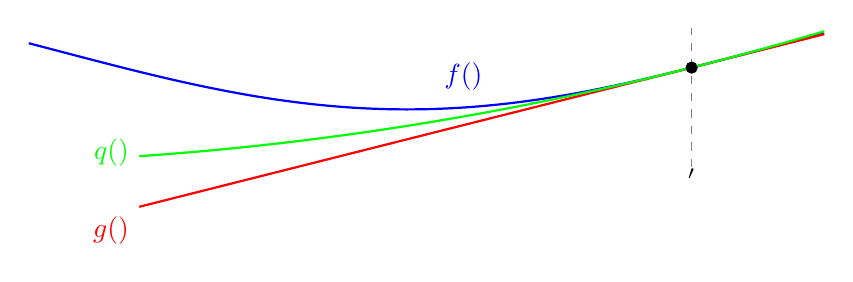
\begin{tikzpicture}[x=0.5cm]
		\begin{axis}[
			hide axis,
			xmin=3, xmax=6,
			ymin=0, ymax=6,
			domain=0:6,
			samples=100,
			width=10cm,
			height=6cm,
			clip=false
			]
		% Original nonlinear function h(x)
			\addplot[blue, thick, domain=3:6.6] {2 + sin(deg(x))} 
			node[pos=0.5, above right, yshift=3pt] {$f(\featurevec)$};
		% Tangent line as local linear approximation at x = 3
		% h(3) = 2 + sin(3), h'(3) = cos(3)
			\addplot[red, thick, domain=3.5:6.6] 
			{2 + sin(deg(6)) + cos(deg(6))*(x - 6)}
			node[pos=0, below left] {$g(\featurevec)$};
                %%%%%%%%%%%%%%%%%%%%%%%%%%%%%%%%%%%%%%%%%%%%%%%%
                \addplot[green, thick, domain=3.5:6.6]
                {2 + sin(deg(6)) + cos(deg(6))*(x - 6) - 0.5*sin(deg(6))*(x - 6)^2}
			node[pos=0, below left, yshift=10pt] {$q(\featurevec)$};
                %%%%%%%%%%%%%%%%%%%%%%%%%%%%%%%%%%%%%%%%%%%%%%%%
		% Mark point of approximation
			\addplot[mark=*] coordinates {(6, {2 + sin(deg(6))})};
			    % Vertical dashed line (ruler) at x = 3
			\addplot[dashed, gray] coordinates {(6,0) (6,2.4)};
			\node at (axis cs:6, -0.2) {$\featurevec'$};
			    % Plot the two points
			    % Coordinates of the two points
			\pgfmathsetmacro{\xA}{-1.5}
			\pgfmathsetmacro{\xB}{3}
			\pgfmathsetmacro{\yA}{2 + sin(deg(\xA))}
			\pgfmathsetmacro{\yB}{2 + sin(deg(\xB))}
		\end{axis}
		\vspace*{-10mm}
	\end{tikzpicture}
		\vspace*{-5mm}
	\end{center}
	\caption{
		Eine \gls{function} $f(\featurevec)$, die an einem Punkt $\featurevec'$ hinreichend 
		\gls{smooth} ist, kann lokal durch eine \gls{quadfunc} $q(\featurevec)$ approximiert werden, 
		die eine genauere Näherung als eine lineare \gls{function} $g(\featurevec)$ liefert. 
		\label{fig_quadapprox_hessian_dict}}
\end{figure}
		Die Hesse-Matrix $\nabla^2 f(\featurevec')$ kann verwendet werden, um eine 
		\gls{quadfunc}
		$$q(\featurevec) = (1/2) (\featurevec- \featurevec')^{T} \underbrace{\nabla^2 f(\featurevec')}_{\text{Hesse-Matrix}} 
		(\featurevec- \featurevec') +  (\featurevec- \featurevec')^{T} \underbrace{\nabla f(\featurevec')}_{\text{Gradient}} 
		+ f(\featurevec')$$
		zu berechnen, die $f$ lokal um $\featurevec'$ approximiert.\cite{MathematikOnline_HesseMatrix}
        		\\
		Siehe auch: \gls{differentiable}, \gls{matrix}, \gls{function}, \gls{quadfunc}. }, 
	first={Hesse-Matrix},
	type=math,
	text={Hesse-Matrix}
}

\newglossaryentry{continuous}
{name={stetig}, 
description={Eine \gls{function}\index{stetig} $f: \mathbb{R}^{\nrfeatures} \to \mathbb{R}$ heißt 
	stetig an einem Punkt $\featurevec' \in \mathbb{R}^{\nrfeatures}$, wenn für jedes 
	$\epsilon > 0$ ein $\delta > 0$ existiert, so dass für alle 
	$\featurevec \in \mathbb{R}^{\nrfeatures}$ mit 
	$\normgeneric{\featurevec - \featurevec'}{2} < \delta$ gilt: 
	$|f(\featurevec) - f(\featurevec')| < \epsilon$ \cite{RudinBookPrinciplesMatheAnalysis}. 
	Mit anderen Worten: Wir können $f(\featurevec)$ beliebig nahe an 
	$f(\featurevec')$ bringen, indem wir $\featurevec$ hinreichend nahe an 
	$\featurevec'$ wählen. Ist $f$ an jedem Punkt 
	$\featurevec' \in \mathbb{R}^{\nrfeatures}$ stetig, so heißt $f$ 
	stetig auf $\mathbb{R}^{\nrfeatures}$. 
	Der Begriff der stetigen \gls{function} lässt sich auf 
	\glspl{function} zwischen allgemeinen \gls{metric} Räumen 
	natürlich verallgemeinern \cite{RudinBookPrinciplesMatheAnalysis}.\\
		Siehe auch: \gls{euclidspace}, \gls{metric}.},
	first={stetig},
	type=math,
	text={stetig}
}


\newglossaryentry{linearmap}
{name={lineare Abbildung}, plural={lineare Abbildungen},
 description={Eine \textbf{lineare Abbildung}\index{lineare Abbildung} $f: \mathbb{R}^n \rightarrow \mathbb{R}^m$ 
	ist eine \gls{funktion}, die folgende Eigenschaften erfüllt:
	\begin{itemize}
		\item \textbf{Additivität:} $f(\vx + \vy) = f(\vx) + f(\vy)$
		\item \textbf{Homogenität:} $f(c\vx) = c f(\vx)$ für alle \glspl{vector} $\vx, \vy \in \mathbb{R}^n$ 
		und Skalare $c \in \mathbb{R}$
	\end{itemize}
	Daraus folgt insbesondere $f(\mathbf{0}) = \mathbf{0}$.
	Jede lineare \gls{map} kann als \gls{matrix}-Multiplikation dargestellt werden: 
	$$f(\vx) = \mA \vx \quad \text{für eine} \quad \mA \in \mathbb{R}^{m \times n}.$$

	Die Gesamtheit der reellwertigen linearen \glspl{map} eines gegebenen Eingaberaums bildet ein 
	\gls{linmodel}, das in vielen \glspl{ml}-Verfahren eingesetzt wird.
	\\
	Siehe auch: \gls{map}, \gls{funktion}, \gls{vector}, \gls{matrix}, \gls{linmodel}, \gls{ml}.},
	first={lineare Abbildung},
	text={lineare Abbildung}
}

\newglossaryentry{vector}
{name={Vektor},
	description={Ein \index{vector} Vektor ist ein Element eines \gls{vectorspace}. 
		In the context of \gls{ml}, a particularly important example of a \gls{vectorspace} 
		is the \gls{euclidspace} $\mathbb{R}^{\nrfeatures}$, where $\nrfeatures \in \mathbb{N}$ 
		is the (finite) dimension of the space. A vector $\vx \in \mathbb{R}^{\nrfeatures}$ 
		can be represented as a list or one-dimensional array of real numbers, i.e., 
		$x_1, \ldots, x_{\nrfeatures}$ with $x_\featureidx \in \mathbb{R}$ for 
		$\featureidx = 1, \ldots, \nrfeatures$. The value $x_\featureidx$ is the $\featureidx$-th 
		entry of the vector $\vx$. It can also be useful to view a vector $\vx \in \mathbb{R}^{\nrfeatures}$ 
		as a \gls{function} that maps each index $\featureidx \in \{1, \ldots, \nrfeatures\}$ 
		to a value $x_\featureidx \in \mathbb{R}$, i.e., $\vx: \featureidx \mapsto x_\featureidx$. 
		This perspective is particularly useful for the study of \glspl{kernelmethod}.
		\begin{figure}[H]
			% Left: Stem plot
			\begin{minipage}[c]{0.48\textwidth}
				\centering 
				2, -1, 3, 0, -2, 1
				\begin{minipage}{\textwidth}
				\vspace{5ex}
				\centering
				{\selectfont (a)}
				\end{minipage}
			\end{minipage}
			\hfill
			% Right: Column vector
			\begin{minipage}{0.48\textwidth}
			\centering
			\begin{tikzpicture}
			\begin{axis}[
    				width=6.5cm,
    				height=5cm,
    				title={},
    				xlabel={index $\featureidx$},
    				ylabel={$x_\featureidx$},
   		 		ymin=-3.5, ymax=3.5,
    				xmin=0.5, xmax=6.5,
   	 			xtick={1,2,3,4,5,6},
    				ytick={-3,-2,-1,0,1,2,3},
    				axis x line=bottom,        % <-- horizontal axis at y=0
    				axis y line=left,          % <-- vertical axis on the left
    				grid=both,
    				major grid style={dotted, gray!60},
    				enlargelimits=0.1
			]
			\addplot+[ycomb, thick, mark=*]
    			coordinates {
        				(1,2)
        				(2,-1)
       	 			(3,3)
        				(4,0)
        				(5,-2)
        				(6,1)
    			};
			\end{axis}
			\node at (2,-2.5) {(b)};
			\end{tikzpicture}
			\end{minipage}
			\caption{Two equivalent views of a vector $\vx= \big( 2, -1, 3, 0, -2, 1 \big)^{T} \in \mathbb{R}^{6}$.
			(a) As a numeric array. (b) As a \gls{map} $\featureidx \mapsto x_\featureidx$.}
			\label{fig:vector-function-dual_dict}
		\end{figure}
		See also: \gls{vectorspace}, \gls{euclidspace}, \gls{linearmap}.},
	first={vector},
	type=math,
	firstplural={vectors},
	plural={vectors},
	text={vector}
}


\newglossaryentry{vectorspace}
{name={vector space},
	description={A\index{vector space} \gls{vector} space $\mathcal{V}$ (also called linear space) 
	is a collection of elements, called \glspl{vector}, along with two operations: 
    addition (denoted by $\vv+\vw$) of two vectors $\vv,\vw$ and multiplication 
	(denoted $c\cdot \vv$) of a vector $\vv$ with a scalar $c$ who belongs to some 
	number field (a typical choice for this field is $\mathbb{R}$). The defining 
	property of a vector space is that it is closed under these operations, i.e.,
		\begin{itemize}
			\item If $\vv, \vw \in \mathcal{V}$, then $\vv + \vw \in \mathcal{V}$.
			\item If $\vv \in \mathcal{V}$ and $c \in \mathbb{R}$, then $c \vv \in \mathcal{V}$.
			\item In particular, $\mathbf{0} \in \mathcal{V}$.
		\end{itemize}
		\begin{figure}[ht]
		\centering
			\begin{tikzpicture}[>=Stealth, scale=1.2]
				  % Coordinates
  			\coordinate (O) at (0,0);            % Origin
  			\coordinate (V) at (2,1.5);          % vector v
  			\coordinate (W) at (1,3);            % vector w
  			\coordinate (VplusW) at (3,4.5);     % v + w
  			\coordinate (HalfV) at (1,0.75);     % 0.5 * v
  			\draw[->, thick, blue] (O) -- (V) node[pos=1, right] {$\vv$};
  			\draw[->, thick, red] (O) -- (W) node[pos=1, left] {$\vw$};
  			\draw[->, thick, purple] (O) -- (VplusW) node[pos=0.99, above right] {$\vv+\vw$};
  			\draw[dashed, red] (V) -- (VplusW);
  			\draw[dashed, blue] (W) -- (VplusW);
  			\draw[->, thick, orange] (O) -- (HalfV) node[midway, right] {$0.5\vv$};
			% Filled dots
  			\filldraw[black] (O) circle (2pt) node[below left] {$\mathbf{0}$};  % origin
  			\filldraw[blue] (V) circle (2pt);         % v
  			\filldraw[red] (W) circle (2pt);          % w
  			\filldraw[purple] (VplusW) circle (2pt);  % v + w
  			\filldraw[orange] (HalfV) circle (2pt);   % 0.5v
			\end{tikzpicture}
			\caption{A vector space $\mathcal{V}$ is a collection of vectors such that scaling 
			and adding them always yields another vector in $\mathcal{V}$. In \gls{ml} applications, 
			 vectors are used to represent \glspl{datapoint} (or their \glspl{featurevec}) and 
			 invariances (or symmetries) of \glspl{model}.}
			\label{fig:vector-ops_dict}
		\end{figure}
		A common example of a vector space is the \gls{euclidspace} $\mathbb{R}^n$, which is widely used in 
		\gls{ml} to represent \glspl{model} and \glspl{dataset}.
		\\
		See also: \gls{vector}, \gls{euclidspace}, \gls{linmodel}, \gls{linearmap}.},
	first={vector space},
	type=math,
	text={vector space}
}


\newglossaryentry{stochastic}
{name={stochastic},
	description={We refer to a \index{stochastic} method as stochastic if it involves a 
		random component or is governed by probabilistic laws. \Gls{ml} methods use randomness 
		to reduce computational complexity (e.g., see \gls{stochGD}) or 
		to capture \gls{uncertainty} in \glspl{probmodel}.
		\\
		See also: \gls{stochGD}, \gls{uncertainty}, \gls{probmodel}.},
	first={stochastic},
	text={stochastic}
}

\newglossaryentry{stochproc}
{name={stochastic process},
	description={
		A \gls{stochastic} process\index{stochastic process} is a collection of 
		\glspl{rv} defined on a common \gls{probspace}, indexed by some set 
		$\mathcal{I}$ \cite{papoulis,GrayProbBook,Brockwell91}. The index set 
		$\mathcal{I}$ typically represents time or space, allowing to represent 
		random phenomena that evolve across time or spatial dimensions—for example, 
		sensor noise or financial time series. Stochastic processes are not limited 
		to temporal or spatial settings. For instance, random \glspl{graph} such as 
		the \gls{ergraph} or the \gls{sbm} 
		can also be viewed as stochastic processes. Here, the index set $\mathcal{I}$ 
		consists of node pairs that index \glspl{rv} whose values encode 
		the presence or weight of an edge between two nodes. Moreover, \gls{stochastic} 
		processes naturally arise in the analysis of \glspl{stochalgorithm}, 
		such as \gls{stochGD}, which construct a sequence of \glspl{rv}. 
		\\
		See also:  \gls{rv}, \gls{sbm}, \gls{stochGD}, \gls{uncertainty}, \gls{probmodel}.},
	first={stochastic process},
	firstplural={stochastic processes},
	plural={stochastic processes},
	text={stochastic process}
}

\newglossaryentry{characteristicfunc}
{name={characteristic function},
	description={The characteristic \gls{function}\index{characteristic function} 
		of a real-valued \gls{rv} $x$ is the \gls{function} \cite[Sec. 26]{BillingsleyProbMeasure}
		$$ \phi_{x}(t) \defeq \expect { \exp\,(j t x) } \mbox{ with } j = \sqrt{-1}.$$
	 	The characteristic \gls{function} uniquely determines the \gls{probdist} of $x$. 
		\\
		See also: \gls{rv}, \gls{probdist}.},
	first={characteristic function},
	firstplural={characteristic functions}, 
	plural={characteristic functions},
	text={characteristic function}
}

\newglossaryentry{entropy}
{name={entropy},
	description={Entropy\index{entropy} quantifies the \gls{uncertainty} or unpredictability associated with an \gls{rv} \cite{coverthomas}. 
		For a discrete \gls{rv} $x$ taking on values in a finite set $\mathcal{S} = \{x_1, \ldots, x_n\}$ with 
		a \gls{probability} mass \gls{function} $p_i \defeq \prob{x = x_i}$, the entropy is defined as
		\[
		H(x) \defeq -\sum_{i=1}^n p_i \log p_i.
		\]
		Entropy is maximized when all outcomes are equally likely, and minimized (i.e., zero) 
		when the outcome is deterministic. A \gls{generalization} of the concept of entropy for continuous 
		\glspl{rv} is \gls{diffentropy}. 
		\\
		See also: \gls{uncertainty}, \gls{probmodel}.},
	first={entropy},
	text={entropy}
}

\newglossaryentry{diffentropy}
{name={differential entropy},
	description={For\index{differential entropy} a real-valued \gls{rv} $\featurevec \in \mathbb{R}^{\nrfeatures}$ 
		with a \gls{pdf} $p(x)$, the differential \gls{entropy} is defined as \cite{coverthomas}
		\[
		h(\featurevec) \defeq - \int p(\featurevec) \log p(\featurevec) \, d\featurevec.
		\]
		Differential \gls{entropy} can be negative and lacks some properties of \gls{entropy} for 
		discrete-valued \glspl{rv}, such as invariance under a change of variables \cite{coverthomas}. 
		Among all \glspl{rv} with a given \gls{mean} $\meanvecgeneric$ and \gls{covmtx} $\covmtxgeneric$, 
		$h(\featurevec)$ is maximized by $\featurevec \sim \mvnormal{\meanvecgeneric}{\covmtxgeneric}$. 
		\\
		See also: \gls{uncertainty}, \gls{probmodel}.},
	first={differential entropy},
	text={differential entropy}
}

	\newglossaryentry{minimum}
{name=Minimum,
 description={Bei einer gegebenen Menge and reeller Zahlen, ist das Minimum \index{minimum} das kleinste dieser Zahlen.},
 first={Minimum},text={Minimum}, plural={Minima}
}

\newglossaryentry{co-domain}
{name={Zielmenge}, 
	description={Die Zielmenge\index{Zielmenge} einer \gls{function} 
	$f: \mathcal{U} \rightarrow \mathcal{V}$ ist die Menge $\mathcal{V}$, 
	in die $f$ die Elemente ihres Definitionsbereichs $\mathcal{U}$ abbildet.  
	\\
	Siehe auch: \gls{function}, \gls{domain}, \gls{map}.},
	first={Zielmenge},
	firstplural={Zielmengen}, 
	type=math, 
	plural={Zielmengen},
	text={Zielmenge}
}

\newglossaryentry{domain}
{name={Definitionsbereich}, 
	description={Der Definitionsbereich\index{Definitionsbereich} einer \gls{function} 
	$f: \mathcal{U} \rightarrow \mathcal{V}$ ist die Menge $\mathcal{U}$, 
	aus der $f$ seine Eingaben nimmt.  
	\\
	Siehe auch: \gls{function}, \gls{co-domain}, \gls{map}.},
	first={Definitionsbereich},
	firstplural={Definitionsbereiche}, 
	type=math, 
	plural={Definitionsbereiche},
	text={Definitionsbereich}
}


\newglossaryentry{function}
{name={Funktion}, 
	description={Eine Funktion\index{Funktion} zwischen zwei Mengen $\mathcal{U}$ und $\mathcal{V}$ ordnet  
	jedem Element $u \in \mathcal{U}$ genau ein Element $f(u) \in \mathcal{V}$ zu \cite{RudinBookPrinciplesMatheAnalysis}.
	Wir schreiben dies als 
	$$f: \mathcal{U} \rightarrow \mathcal{V}: u \mapsto f(u)$$ 
	wobei $\mathcal{U}$ der \gls{domain} und $\mathcal{V}$ der \gls{co-domain} von $f$ entspricht. 
	Das heißt, eine Funktion $f$ definiert für jedes Eingabeelement $u \in \mathcal{U}$ genau ein Ausgabeelement $f(u) \in \mathcal{V}$ (siehe Abb. \ref{fig_function_dict}).
	\begin{figure}[H]
		\centering
		\begin{tikzpicture}[>=stealth, node distance=1.2cm and 2.5cm]
			\tikzset{dot/.style={circle, fill=black, inner sep=1.2pt}}
			\node (A) [dot, label=left:$a$] {};
			\node (B) [dot, below=of A, label=left:$b$] {};
			\node (C) [dot, below=of B, label=left:$c$] {};
			\node (1) [dot, right=4cm of A, label=right:$\star$] {};
			\node (2) [dot, below=of 1, label=right:$\circ$] {};
			\node (3) [dot, below=of 2, label=right:$\otimes$] {};
			\node[draw=blue!70, thick, ellipse, inner sep=0.5cm, fit=(A)(B)(C), label=above:$\mathcal{U}$] {};
			\node[draw=green!70!black, thick, ellipse, inner sep=0.5cm, fit=(1)(2)(3), label=above:$\mathcal{V}$] {};
			\draw[->] (A) -- (2);
			\draw[->] (B) -- (1);
			\draw[->] (C) -- (2);
		\end{tikzpicture}
		\caption{Eine Funktion \( f \colon \mathcal{U} \to \mathcal{V} \), die jedes Element 
		des \gls{domain} $\mathcal{U} =  \{a,b,c\}$ genau einem Element der 
		\gls{co-domain} $\mathcal{V} = \{\star,\circ,\otimes\}$ zuordnet. \label{fig_function_dict}}
	\end{figure}},
	first={Funktion},
	firstplural={Funktionen}, 
	type=math, 
	plural={Funktionen},
	text={Funktion}
}



\newglossaryentry{map}
{name={map}, 
	description={We\index{map} use the term map as a synonym for \gls{function}.
		\\
		See also: \gls{function}.},
	first={map},
	firstplural={maps},	
	plural={maps},
	text={map}
}

\newglossaryentry{attention}
{name={attention}, 
	description={In einigen \gls{ml}-Anwendungen\index{attention} bestehen \glspl{datapoint} 
	aus kleineren Einheiten, die als \glspl{token} bezeichnet werden. Zum Beispiel besteht ein Satz 
	aus Wörtern, ein Bild aus Pixel-Patches und ein Netzwerk aus Knoten. Im Allgemeinen 
	sind die \glspl{token}, die einen einzelnen \gls{datapoint} bilden, nicht voneinander unabhängig. 
	Stattdessen hängt jedes \gls{token} eines \gls{datapoint} von bestimmten anderen \glspl{token} ab 
	(beziehungsweise "pay attention" auf sie). \Glspl{probmodel} bieten einen prinzipiellen Rahmen, um 
	solche Abhängigkeiten darzustellen und zu analysieren \cite{Blei2003}. Attention-Mechanismen verfolgen 
	einen direkteren Ansatz ohne explizite Bezugnahme auf ein \gls{probmodel}. Die Grundidee besteht darin, 
	die Beziehung zwischen zwei Tokens $\nodeidx$ und $\nodeidx'$ mittels einer parametrisierten 
	\gls{function} $f^{(\weights)}(\nodeidx,\nodeidx')$ darzustellen, wobei die \glspl{parameter} 
	$\weights$ über eine Variante von \gls{erm} gelernt werden. Praktische Attention-Mechanismen 
	unterscheiden sich in der genauen Wahl des Attention-\gls{model} $f^{(\weights)}(\nodeidx,\nodeidx')$ 
	sowie der verwendeten \gls{erm}-Variante. Eine weit verbreitete Familie von Attention-Mechanismen 
	definiert die \glspl{parameter} $\weights$ in Form von zwei \glspl{vector}, die jedem Token $\nodeidx$ 
	zugeordnet sind, nämlich einem Query-\gls{vector} $\vq^{(\nodeidx)}$ und einem Key-\gls{vector} $\vk^{(\nodeidx')}$. 
	Für ein gegebenes Token $\nodeidx$ mit Query $\vq^{(\nodeidx)}$ und ein anderes Token $\nodeidx'$ mit Key 
	$\vk^{(\nodeidx')}$ quantifiziert die Größe 
	$\big( \vq^{(\nodeidx)} \big)^{\top} \vk^{(\nodeidx')}$, in welchem Ausmaß Token $\nodeidx$ auf 
	Token $\nodeidx'$ "attentiert" bzw. von ihm abhängt (siehe Abb. \ref{fig_attention_dict}).
	\begin{figure}[H]
		\centering
		\begin{tikzpicture}[>=stealth, node distance=0.2cm and 0.2cm,
		every node/.style={inner sep=2pt, font=\large}, baseline]
		% Words (sentence: All human beings are born free and equal.)
		\node (w1) [draw, fill=gray!10, rounded corners] {All};
		\node (w2) [draw, fill=gray!10, right=of w1, rounded corners] {human};
		\node (w3) [draw, fill=gray!10, right=of w2, rounded corners] {beings};
		\node (w4) [draw, fill=gray!10, right=of w3, rounded corners] {are};
		\node (w5) [draw, fill=gray!10, right=of w4, rounded corners] {born};
		\node (w6) [draw, fill=gray!10, right=of w5, rounded corners] {free};
		\node (w7) [draw, fill=gray!10, right=of w6, rounded corners] {and};
		\node (w8) [draw, fill=blue!20, right=of w7, rounded corners] {equal};
		\node[font=\footnotesize, below=0.15cm of w8, align=center] (labeli) {$\nodeidx$ \\ $\vq^{(\nodeidx)},\ \vk^{(\nodeidx)}$};
		\node[font=\footnotesize, below=0.15cm of w1, align=center] (labelii) {$\nodeidx'$ \\ $\vq^{(\nodeidx')},\ \vk^{(\nodeidx')}$};
		\node (eqTop) [above=1.8cm of w8] {};
		\draw[->, thick, opacity=0.3] (w8.north) .. controls +(up:1.0cm) and +(up:1.0cm) .. (w6.north);
		\draw[->, thick, opacity=0.3] (w8.north) .. controls +(up:1.2cm) and +(up:1.0cm) .. (w5.north);
		\draw[->, thick, opacity=1]  (w8.north)  .. controls +(up:1.8cm) and +(up:1.0cm) ..  node[midway, text=black, above] {$f^{(\weights)}(\nodeidx,\nodeidx')$}  (w1.north);
		\end{tikzpicture}
		\caption{Attention-Mechanismen lernen eine parametrisierte \gls{function} $f^{(\weights)}(\nodeidx,\nodeidx')$, um zu messen, 
		wie stark Token $\nodeidx$ auf Token $\nodeidx'$ "attentiert". Eine weit verbreitete Konstruktion von 
		$f^{(\weights)}(\nodeidx,\nodeidx')$ nutzt Query- und Key-\glspl{vector}, bezeichnet durch 
		$\vq^{(\nodeidx)}$ und $\vk^{(\nodeidx)}$, die jedem Token $\nodeidx$ zugeordnet werden \cite{vaswani2017attention}. 
		\label{fig_attention_dict}}
	\end{figure}
	See also: \gls{function}, \gls{nlp}, \gls{token}.},
	first={attention},
	text={attention}
}

\newglossaryentry{transformer}
{name={transformer},
 description={Im Kontext von \gls{ml} bezeichnet der Begriff transformer\index{transformer} 
 	ein \glspl{ann}, das eine Form von \gls{attention}-Mechanismus verwendet, 
 	um Abhängigkeiten zwischen \glspl{token} zu erfassen \cite{vaswani2017attention}. 
 	Der \gls{attention}-Mechanismus unterscheidet Transformer von früheren 
	\glspl{model}, die für sequentielle \gls{data}, wie z. B. \glspl{rnn}, eingesetzt wurden. 
	Ein Transformer-\gls{ann} kombiniert häufig mehrere \gls{attention}-\glspl{layer}, 
	die über traditionelle \gls{layer}-Architekturen integriert werden.\\
	See also: \gls{nlp}, \gls{attention}.
  }, 
 first = {transformer}, 
 text={transformer},
 firstplural={transformers}, 
 plural = {transformers}
}

\newglossaryentry{rnn}
{name={recurrent neural network (RNN)},
 description={Ein \index{recurrent neural network (RNN)} RNN 
 	ist ein spezieller Typ eines \gls{ann}, der für die Verarbeitung von 
 	\gls{data} entwickelt wurde, die als Sequenz von \glspl{token} vorliegt. 
 	Ein RNN besitzt einen internen Hidden-State, der bei der Verarbeitung neuer 
 	\glspl{token} rekurrent aktualisiert wird. Durch diese rekurrente Struktur kann 
 	Information über verschiedene Zeitschritte hinweg propagiert werden, wodurch 
 	RNNs für Aufgaben wie Spracherkennung, Sprachmodellierung oder Zeitreihenprognose 
 	besonders geeignet sind. 
 	Die sequentielle Berechnung begrenzt jedoch die Parallelisierbarkeit und 
 	erhöht die Komplexität bei der Anwendung von \glspl{gdmethod}. Varianten wie 
 	Long Short-Term Memory (LSTM) und Gated Recurrent Unit (GRU) 
 	adressieren diese Einschränkungen, indem sie den Informationsfluss 
 	über längere Zeiträume stabilisieren.}, 
 first = {recurrent neural network (RNN)},
 text={RNN}
}

\newglossaryentry{llm}
{name={large language model (LLM)},
 description={A\index{large language model (LLM)} LLM is an umbrella term for \gls{ml} 
               methods that use high-dimensional \gls{ml} \glspl{model} (with billions 
			   of \glspl{modelparam}) trained on large collections of text \gls{data}. 
 			  LLMs are used to analyze or generate sequences of \glspl{token} which 
               constitute text \gls{data}. Many current LLMs use some variant of 
			   a \gls{transformer} that is trained via self-supervised learning:  
			   The training is based on the task of predicting a few words that 
			   are intentionally removed from a large text corpus. Thus, we can 
			   construct \glspl{labeled datapoint} simply by selecting some words 
			   from a given text as \glspl{label} and the remaining words as \glspl{feature} 
			   of \glspl{datapoint}. This construction requires 
		       very little human supervision and allows for generating sufficiently 
		       large \glspl{trainset} for LLMs.\\ 
			   See also: \gls{nlp}, \gls{token}, \gls{transformer}.}, 
  first = {LLM}, 
  firstplural={LLMs}, 
  text = {LLM}, 
  plural = {LLMs} 
}

\newglossaryentry{selfsupervisedlearning}
{name={selbstüberwachtes Lernen},
 description={Selbstüberwachtes Lernen \index{selbstüberwachtes Lernen} verwendet einen Teil 
 	der \glspl{feature} eines \gls{datapoint} als \gls{label}. Zum Beispiel kann, 
 	wenn ein \gls{datapoint} aus einem Satz innerhalb eines Textdokuments besteht, 
 	das letzte Wort des Satzes als \gls{label} verwendet werden, das aus allen 
 	vorhergehenden Wörtern vorhergesagt werden soll (die die \glspl{feature} des 
 	\gls{datapoint} bilden). Eine Hauptanwendung des selbstüberwachten Lernens 
 	liegt im Bereich der \gls{nlp} für das Training von \glspl{llm} auf Basis großer 
 	Textsammlungen.\\
 	See also: \gls{feature}, \gls{label}, \gls{llm}.}, 
 first = {selbstüberwachtes Lernen}, 
 text = {selbstüberwachtes Lernen}
}


\newglossaryentry{optproblem}
{name={optimization problem}, 
	description={An\index{optimization problem} optimization problem is a mathematical 
		   structure consisting of an \gls{objfunc} $f: \mathcal{U} \rightarrow \mathcal{V}$ 
		   defined over an optimization variable $\weights \in \mathcal{U}$, together with a 
		   feasible set $\mathcal{W} \subseteq \mathcal{U}$. The co-domain $\mathcal{V}$ is 
		   assumed to be ordered, meaning that for any two elements $\mathbf{a}, \mathbf{b} \in \mathcal{V}$, 
		   we can determine whether $\mathbf{a} < \mathbf{b}$, $\mathbf{a} = \mathbf{b}$, 
		   or $\mathbf{a} > \mathbf{b}$. The goal of optimization is to find those values $\weights \in \mathcal{W}$ 
		   for which the objective $f(\weights)$ is extremal—i.e., minimal or maximal \cite{BoydConvexBook}, \cite{BertsekasNonLinProgr}, \cite{nesterov04}.
		   \\
		   See also: \gls{objfunc}.},
	first={optimization problem},
	firstplural={optimization problems}, 
	plural={optimization problems}, 
	text={optimization problem}
}

\newglossaryentry{optmethod}
{name={optimization method},
	description={An\index{optimization method} optimization method is an \gls{algorithm} that 
		reads in a representation of an \gls{optproblem} and delivers an (approximate) solution 
		as its output \cite{BoydConvexBook}, \cite{BertsekasNonLinProgr}, \cite{nesterov04}.
		 \\
		 See also: \gls{algorithm}, \gls{optproblem}.},
	first={optimization method},
	firstplural={optimization methods}, 
	plural={optimization methods}, 
	text={optimization method}
}

\newglossaryentry{convexopt} {
    name={konvexe Optimierung},
    description={Die konvexe Optimierung\index{konvexe Optimierung} beschäftigt sich mit der Formulierung, den Eigenschaften und effizienten Lösungsmethoden für \gls{convex} \glspl{optproblem} \cite{BoydConvexBook}. Ein \gls{convex} \gls{optproblem} (definiert auf dem \gls{euclidspace} $\mathbb{R}^{\nrfeatures}$) besteht aus einer \gls{convex} \gls{objfunc} $f: \mathbb{R}^{\nrfeatures} \rightarrow \mathbb{R}$ und einer \gls{convex} zulässigen Menge $\mathcal{C}$ für die Optimierungsvariable $\weights$. Es kann kompakt geschrieben werden als \cite{BoydConvexBook} 
    $$
    \min_{\weights \in \mathcal{C}} f(\weights).
    $$
    Alternativ kann ein \gls{convex} \gls{optproblem} in Form von \gls{convex}en Nebenbedingungsfunktionen $g_1,\ldots,g_k$ ausgedrückt werden:
    \begin{align}
    \min_{\weights \in \mathbb{R}^{\nrfeatures}} & f(\weights) \nonumber \\
    \text{s.d.} \quad & g_{\sampleidx}(\weights) \leq 0, \quad \sampleidx=1,\,\ldots,\,k. \label{equ_def_convx_opt_constr_dict}
    \end{align}
    \begin{figure}
    \centering
    \begin{tikzpicture}[>=stealth, scale=1.0]
    % Achsen
    \draw[->] (-3,0) -- (5.2,0) node[below] {$\vc$};
    \draw[->] (0,-0.2) -- (0,4.2) node[left] {$t$};

    % Exponentielle Grenze: t = 3 e^{-g}
    \draw[thick, domain=-1:3, smooth, variable=\x, name path=boundary] plot ({\x},{exp(-\x)});

    % Transparente Epigraphregion (oberhalb der Kurve)
    \path[fill=gray!40, opacity=0.4] (-1,3) -- (-1,{exp(1)}) -- plot[domain=-1:3] ({\x},{exp(-\x)}) -- (3,3) -- cycle;

    % Schnittpunkt mit vertikaler Achse (g=0): markieren und f^* beschriften
    \fill (0,1) circle (1.6pt) node[left] {$f^{\ast}$};

    % Tangente bei g=1: Steigung = -e^{-1}, durch (1, e^{-1})
    \draw[dashed, domain=-1:3, smooth, variable=\x] plot ({\x},{(2/exp(1)) - (1/exp(1))*\x});

    % Punkt der Tangente markieren
    \fill (1,{1/exp(1)}) circle (1.2pt);

    % Beschriftung der schattierten Region
    \node at (2.6,2.5) {$\mathcal{A}$};
    \node [below,yshift=-3pt] at (0,-0.2) {$\mathbf{0}$};
    \end{tikzpicture}
    \caption{Ein \gls{convex} \gls{optproblem} \eqref{equ_def_convx_opt_constr_dict} kann durch eine Menge $\mathcal{A}$ dargestellt werden,
	 die aus den erreichbaren Zielwerten $t$ und den Nebenbedingungswerten $\vc=\big(c_{1},\ldots,c_{\nrfeatures}\big)^{T}$ besteht, 
	 d.h., $f(\weights) \leq t, g_{1}(\weights)\leq c_{1},\ldots, g_{k}(\weights) \leq c_{k}$ für ein $\weights \in \mathbb{R}^{\nrfeatures}$.
	 Der optimale Wert $f^{\ast}$ des \gls{optproblem} ist der kleinste $t$, für den $(\mathbf{0},t) \in \mathcal{A}$ gilt.}
    \end{figure}

    Die Formulierung \eqref{equ_def_convx_opt_constr_dict} führt zur Epigraphform \cite[Sec 5.3]{BoydConvexBook}:
    $$
    \inf \big\{ t \in \mathbb{R} : (\mathbf{0}, t) \in \mathcal{A} \big\},
    $$
    mit der Menge
    \begin{align}
    \mathcal{A} \defeq \big\{ (\vc,t) & \in \mathbb{R}^{\nrfeatures} \times \mathbb{R} : f(\weights) \leq t, \, \nonumber \\
    & g_{\sampleidx}(\weights) \leq c_{\sampleidx}, \, \sampleidx = 1,\ldots,k, \text{ für ein } \weights \in \mathbb{R}^{\nrfeatures} \big\}. \nonumber
    \end{align}
    Es kann gezeigt werden, dass, da $f,g_{1},\ldots,g_{k}$ \gls{convex}e \glspl{function} sind, $\mathcal{A}$ eine \gls{convex}e Menge ist \cite[Ch.2]{BoydConvexBook}.
	 Die Menge $\mathcal{A}$ charakterisiert vollständig das \gls{optproblem}~\eqref{equ_def_convx_opt_constr_dict} und kann als \gls{epigraph} der \gls{objfunc}~$f$ eingeschränkt 
	 auf die zulässige Region, definiert durch die Nebenbedingungsfunktionen $g_1,\ldots,g_k$, interpretiert werden.\\
    Siehe auch: \gls{convex}, \gls{optproblem}, \gls{optmethod}.
    },
    first={konvexe Optimierung},
    type=math,
    text={konvexe Optimierung}
}

\newglossaryentry{newtonmethod}{
    name={Newton-Verfahren},
    description={Das Newton-Verfahren\index{Newton-Verfahren} ist ein iteratives \gls{optmethod}, um lokale \glspl{minimum} oder \glspl{maximum} einer \gls{differentiable} \gls{objfunc} $f(\weights)$ zu finden. 
    Ähnlich wie bei \glspl{gdmethod} wird beim Newton-Verfahren eine neue Schätzung $\estparams{\iteridx+1}$ durch Optimierung einer lokalen Näherung von $f(\weights)$ um die aktuelle Schätzung $\estparams{\iteridx}$ berechnet. 
    Im Gegensatz zu \glspl{gdmethod}, die den \gls{gradient} verwenden, um eine lokale lineare Näherung zu bilden, nutzt das Newton-Verfahren die \gls{hessian} \gls{matrix}, um eine lokale quadratische Näherung zu erstellen. 
    Insbesondere wird ab einer Anfangsschätzung $\estparams{0}$ die Schätzung iterativ nach
    \[
    \estparams{\iteridx+1}= \estparams{\iteridx}- \big( \nabla^2 f\big(\estparams{\iteridx}\big) \big)^{-1} \nabla f\big( \estparams{\iteridx} \big), \quad \iteridx=0,\,1,\,\ldots,
    \]
    aktualisiert. Hierbei bezeichnet $\nabla f\big(\estparams{\iteridx} \big)$ den \gls{gradient} und $\nabla^2 f(\weights^{(\iteridx)})$ die \gls{hessian} der \gls{objfunc} $f$. Da die Verwendung einer \gls{quadfunc} als lokale Näherung präziser ist als die lineare Näherung (die ein Spezialfall einer \gls{quadfunc} darstellt), konvergiert das Newton-Verfahren in der Regel schneller als \glspl{gdmethod} (vgl. Abb. \ref{fig_newtonmethod_dict}). 
    Diese schnellere \gls{convergence} geht jedoch mit einem höheren Rechenaufwand der Iterationen einher, da jede Iteration die Inversion der \gls{hessian} erfordert. 
    \begin{figure}[H]
    \centering
    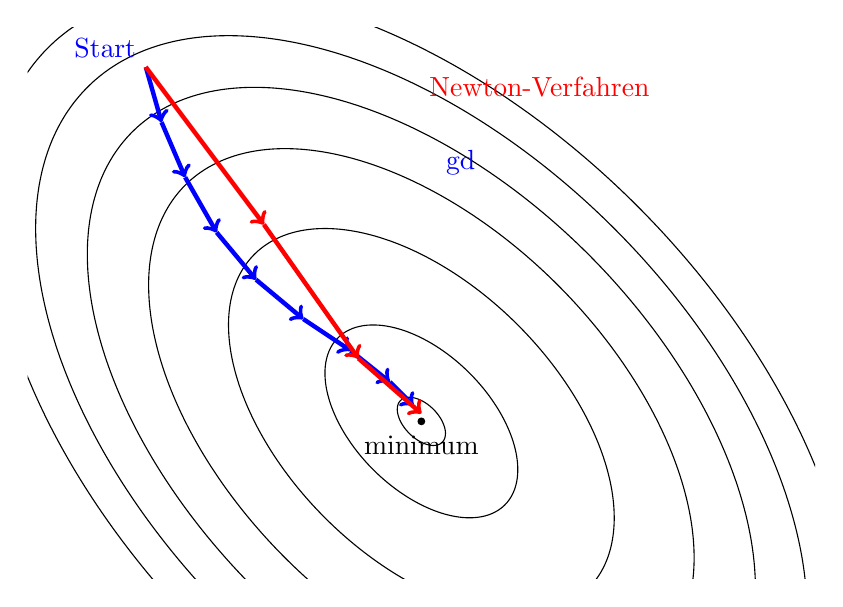
\begin{tikzpicture}[samples=200,smooth]
        \begin{scope}
            \clip(-5,-2) rectangle (5,5);
            % Konturen der Funktion
            \draw[thin] plot[domain=0:360] ({1.5*cos(\x)*sqrt(20/(sin(2*\x)+2))},{1.5*sin(\x)*sqrt(20/(sin(2*\x)+2))});
            \draw[thin] plot[domain=0:360] ({1.5*cos(\x)*sqrt(16/(sin(2*\x)+2))},{1.5*sin(\x)*sqrt(16/(sin(2*\x)+2))});
            \draw[thin] plot[domain=0:360] ({1.5*cos(\x)*sqrt(12/(sin(2*\x)+2))},{1.5*sin(\x)*sqrt(12/(sin(2*\x)+2))});
            \draw[thin] plot[domain=0:360] ({1.5*cos(\x)*sqrt(8/(sin(2*\x)+2))},{1.5*sin(\x)*sqrt(8/(sin(2*\x)+2))});
            \draw[thin] plot[domain=0:360] ({1.5*cos(\x)*sqrt(4/(sin(2*\x)+2))},{1.5*sin(\x)*sqrt(4/(sin(2*\x)+2))});
            \draw[thin] plot[domain=0:360] ({1.5*cos(\x)*sqrt(1/(sin(2*\x)+2))},{1.5*sin(\x)*sqrt(1/(sin(2*\x)+2))});
            \draw[thin] plot[domain=0:360] ({1.5*cos(\x)*sqrt(0.0625/(sin(2*\x)+2))},{1.5*sin(\x)*sqrt(0.0625/(sin(2*\x)+2))});
            % Gradient Descent-Pfad
            \draw[->,blue,ultra thick] (-3.5,4.5) -- (-3.3,3.8);
            \draw[->,blue,ultra thick] (-3.3,3.8) -- (-3,3.1);
            \draw[->,blue,ultra thick] (-3,3.1) -- (-2.6,2.4);
            \draw[->,blue,ultra thick] (-2.6,2.4) -- (-2.1,1.8);
            \draw[->,blue,ultra thick] (-2.1,1.8) -- (-1.5,1.3);
            \draw[->,blue,ultra thick] (-1.5,1.3) -- (-0.9,0.9);
            \draw[->,blue,ultra thick] (-0.9,0.9) -- (-0.4,0.5);
            \draw[->,blue,ultra thick] (-0.4,0.5) -- (-0.1,0.2);
            \node[blue,above left] at (-3.5,4.5) {Start};
            \node[blue,above] at (0.5,3) {\gls{gd}};
            % Newton-Verfahren-Pfad
            \draw[->,red,ultra thick] (-3.5,4.5) -- (-2,2.5);
            \draw[->,red,ultra thick] (-2,2.5) -- (-0.8,0.8);
            \draw[->,red,ultra thick] (-0.8,0.8) -- (0,0.1);
            \node[red,above] at (1.5,4) {Newton-Verfahren};
            \node at (0,0) [circle,fill,inner sep=1pt,label=below:\gls{minimum}] {};
        \end{scope}
    \end{tikzpicture}
    \caption{Vergleich der Pfade von \gls{gd} (blau) und Newton-Verfahren (rot) zum \gls{minimum} einer \gls{lossfunc}. \label{fig_newtonmethod_dict}}
    \end{figure}
    Siehe auch: \gls{optmethod}, \gls{gradient}, \gls{hessian}, \gls{gd}.
    },
    first={newtonmethod},
    type=math,
    text={newtonmethod}
}

\newglossaryentry{hilbertspace}{
    name={Hilbertraum},
    description={Ein \index{Hilbertraum} Hilbertraum $\hilbertspace$ ist ein vollständiger 
    \gls{vectorspace} mit einem Skalarprodukt. Das heißt, $\hilbertspace$ ist ein \gls{vectorspace}, 
    ausgestattet mit einem Skalarprodukt $\innerprod{\cdot}{\cdot}$. 
    Das Skalarprodukt induziert eine Norm $\normgeneric{\cdot}{2}$ über 
    $\normgeneric{\weights}{2} = \sqrt{\innerprod{\weights}{\weights}}$. 
    Darüber hinaus ist $\hilbertspace$ vollständig im Sinne, dass jede 
    \gls{cauchysequence} $\big( \weights^{(\sampleidx)} \big)_{\sampleidx \in \mathbb{N}}$ 
    in $\hilbertspace$ gegen ein Limit $\lim_{\sampleidx \rightarrow \infty} \weights^{(\sampleidx)}$ konvergiert, 
    das ebenfalls in $\hilbertspace$ enthalten ist. 
    \begin{figure}[H]
    \centering
    \begin{tikzpicture}[scale=3]
        \draw[gray!40] (0,0) circle (1);
        \def\ang{35}
        \draw[->,thick] (0,0) -- (1,0) node[below right] {$\vu$};
        \draw[->,thick] (0,0) -- ({cos(\ang)},{sin(\ang)}) node[above] {$\vv$};
        \coordinate (P) at ({cos(\ang)},0);
        \draw[dashed] ({cos(\ang)},{sin(\ang)}) -- (P);
        \draw[->,thick] (0,0) -- (P) node[pos=0.5,below] {$\innerprod{\vv}{\vu} \vu$};
        \draw ($(P)+(0,0.06)$) -- (P) -- ($(P)+(-0.06,0)$);
        \node[right] at ({cos(-\ang)},{sin(-\ang)}) {$\sphere{\nrfeatures} = \{ \weights \in \mathbb{R}^{\nrfeatures}: \innerprod{\weights}{\weights}=1\}$};
    \end{tikzpicture}
    \caption{Für zwei Einheitsvektoren $\vu, \vv \in \sphere{\nrfeatures} \subseteq \mathbb{R}^{\nrfeatures}$ 
    ist das Skalarprodukt $\innerprod{\vu}{\vv}$ der Koeffizient der Projektion 
    von $\vv$ auf den Unterraum $\{ c \vu: c \in \reals \}$, der von $\vu$ aufgespannt wird. 
    Der Betrag $|\innerprod{\vu}{\vv}|$ misst die Norm dieser Projektion.\label{fig_hilbertspace_dict}}
    \end{figure}
    Ein wichtiges Beispiel für einen Hilbertraum ist der \gls{euclidspace} $\mathbb{R}^{\nrfeatures}$ mit dem Skalarprodukt 
    $\innerprod{\weights}{\weights'} = \weights^{\top} \weights'$. \\
    Siehe auch: \gls{vectorspace}.},
    type=math, 
    first={Hilbertraum}, 
    text={Hilbertraum},
    plural={Hilberträume},
    firstplural={Hilberträume}
}

\newglossaryentry{cauchysequence}{
    name={Cauchy-Folge},
    description={Eine \index{Cauchy-Folge} Cauchy-\gls{sequence} ist eine \gls{sequence} 
    $\big( \featurevec^{(\sampleidx)}\big)_{\sampleidx \in \mathbb{N}}$ 
    in einem \gls{metricspace} $\pair{\featurespace}{\metric{\cdot}{\cdot}}$, 
    sodass die Elemente $\featurevec^{(\sampleidx)} \in \featurespace$ 
    sich mit zunehmendem Index beliebig nahe kommen. Anders ausgedrückt \cite[Def. 3.8]{RudinBookPrinciplesMatheAnalysis}:
    \[
    \forall \epsilon > 0, \exists N \in \mathbb{N} \text{ sodass } 
    \forall \sampleidx, \sampleidx' \geq N: \ \metric{\featurevec^{(\sampleidx)}}{\featurevec^{(\sampleidx')}} < \epsilon.
    \] 
    \begin{figure}
    \centering
    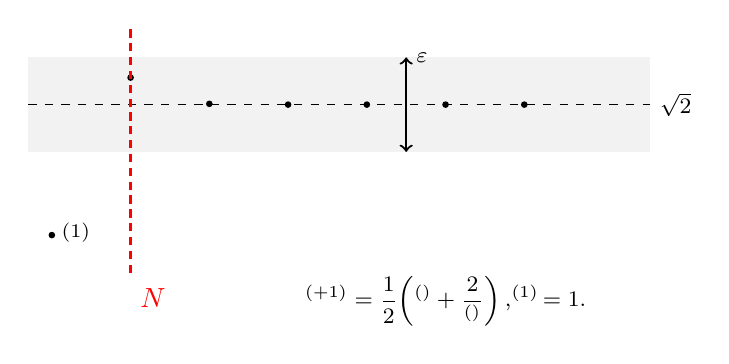
\begin{tikzpicture}[x=1cm,y=4cm]
        \def\srtwo{1.4142}
        \def\eps{0.15}
        \def\nmax{7}
        \fill[gray!30, opacity=0.35] (-0.3,{\srtwo-\eps}) rectangle (\nmax+0.6,{\srtwo+\eps});
        \draw[<->, thick] (4.5,{\srtwo-\eps}) -- (4.5,{\srtwo+\eps}) node[above, right] {\footnotesize{$\varepsilon$}};
        \draw[dashed] (-0.3,\srtwo) -- (\nmax+0.6,\srtwo) node[right] {\footnotesize{$\sqrt{2}$}};
        \fill (0,1.0000) circle (1.2pt) node [right] {$\feature^{(1)}$};
        \fill (1,1.5000) circle (1.2pt);
        \fill (2,1.4167) circle (1.2pt);
        \fill (3,1.4142) circle (1.2pt);
        \fill (4,1.41421) circle (1.2pt);
        \fill (5,1.4142136) circle (1.2pt);
        \fill (6,1.41421356) circle (1.2pt);
        \def\N{1}
        \draw[densely dashed, thick, red] (\N,0.88) -- (\N,1.655);
        \node[right, red] at (\N,0.8) {$N$};
        \node[align=right, anchor=north, font=\small] at (5,0.9) 
        {\footnotesize{$\displaystyle \feature^{(\sampleidx+1)}=\frac{1}{2}\!\left(\feature^{(\sampleidx)}+\frac{2}{\feature^{(\sampleidx)}}\right), \feature^{(1)}=1.$}};
    \end{tikzpicture}
    \caption{Eine Cauchy-\gls{sequence} 
    $\big(\feature^{(\sampleidx)}\big)_{\sampleidx\in\mathbb{N}}$ 
    im \gls{metricspace} $\pair{\mathbb{Q}}{|\cdot|}$. 
    Diese \gls{sequence} wird durch ein \gls{fixedpointiter} erzeugt, um $\sqrt{2}$ zu approximieren. 
    Für alle $\sampleidx \ge N$ liegen die Folgenglieder innerhalb eines Bandes der Breite $\varepsilon$. 
    Beachte, dass die \gls{sequence} in $\mathbb{Q}$ nicht konvergiert, da $\sqrt{2} \notin \mathbb{Q}$ \cite[Beispiel 1.1]{RudinBookPrinciplesMatheAnalysis}.\label{fig:fpit_cauchy_sqrt2_dict}}
    \end{figure}
    Abb.\ \ref{fig:fpit_cauchy_sqrt2_dict} zeigt eine Cauchy-Folge im \gls{metricspace} $\pair{\mathbb{Q}}{|\cdot|}$ der rationalen Zahlen. \\
    Siehe auch: \gls{metricspace}, \gls{sequence}.},
    type=math,
    first={Cauchy-Folge},
    text={Cauchy-Folge},
    plural={Cauchy-Folgen},
    firstplural={Cauchy-Folgen}
}

\newglossaryentry{nonexpansiveop}{
    name={nicht-expansiver Operator},
    description={Ein \index{nicht-expansiver Operator} Operator 
    $\fixedpointop: \hilbertspace \rightarrow \hilbertspace$, definiert auf einem 
    \gls{hilbertspace} $\hilbertspace$, heißt nicht-expansiv, wenn er die Abstände 
    nicht vergrößert. Anders ausgedrückt gilt:
    \[
    \normgeneric{ \fixedpointop \weights - \fixedpointop \weights'}{2} 
    \leq \normgeneric{\weights - \weights'}{2} \quad \text{für alle } \weights, \weights' \in \hilbertspace.
    \]
    Siehe auch: \gls{fixedpointiter}, \gls{contractop}.},
    type=math,
    first={nicht-expansiver Operator},
    text={nicht-expansiver Operator},
    plural={nicht-expansive Operatoren},
    firstplural={nicht-expansive Operatoren}
}


\newglossaryentry{fixedpointiter}
{name={fixed-point iteration},
	description={A\index{fixed-point iteration} fixed-point iteration is an iterative method for solving 
		a given \gls{optproblem}. It constructs a sequence $\weights^{(0)}, \weights^{(1)}, \ldots$ by 
		 repeatedly applying an operator $\fixedpointop$, i.e., 
		 \begin{equation} 
		 	\label{equ_def_fixed_point_dict} 
		 	\weights^{(\iteridx+1)} = \fixedpointop \weights^{(\iteridx)} \mbox{, for } \iteridx=0, 1, \ldots.
		 \end{equation} 
		 The operator $\fixedpointop$ is chosen such that any of its fixed points is a solution 
		 $\widehat{\weights}$ to the given \gls{optproblem}. For example, given a \gls{differentiable} and 
		 \gls{convex} \gls{function} $f(\weights)$, the fixed points of the operator $\fixedpointop: \weights \mapsto \weights - \nabla f(\weights)$ 
		 coincide with the minimizers of $f(\weights)$. In general, for a given \gls{optproblem} with solution $\widehat{\weights}$, 
		 there are many different operators $\fixedpointop$ whose fixed points are $\widehat{\weights}$. 
		 Clearly, we should use an operator $\fixedpointop$ in \eqref{equ_def_fixed_point_dict} that reduces the distance to a solution such that
		 \begin{equation} 
			\nonumber
			\underbrace{\normgeneric{ \weights^{(\iteridx+1)} - \widehat{\netparams}}{2}}_{\stackrel{\eqref{equ_def_fixed_point_dict}}{=} \normgeneric{ \fixedpointop \weights^{(\iteridx)} - \fixedpointop\widehat{\weights}}{2}}  \leq 	\normgeneric{ \weights^{(\iteridx)} - \widehat{\weights}}{2}. 
		\end{equation}
		Thus, we require $\fixedpointop$ to be at least non-expansive, i.e., the iteration \eqref{equ_def_fixed_point_dict} 
		should not result in worse \glspl{modelparam} that have a larger distance to a solution $\widehat{\weights}$. 
		Furthermore, each iteration \eqref{equ_def_fixed_point_dict} should also make some progress, i.e., 
		reduce the distance to a solution $\widehat{\weights}$. This requirement can be made precise using 
		the notion of a \gls{contractop} \cite{Bauschke:2017}, \cite{fixedpoinIsta}. 
		The operator $\fixedpointop$ is a \gls{contractop} if, for some $\contractfac \in [0,1)$,
		\begin{equation} 
			\nonumber
			\normgeneric{ \fixedpointop \weights\!-\!\fixedpointop \weights'}{2}  \leq  \contractfac	\normgeneric{\weights\!-\!\weights'}{2} \mbox{ holds for any } \weights,\weights'.
		\end{equation}
		For a \gls{contractop} $\fixedpointop$, the fixed-point iteration \eqref{equ_def_fixed_point_dict} generates 
		a sequence $\weights^{(\iteridx)}$ that converges quite rapidly. In particular \cite[Th. 9.23]{RudinBookPrinciplesMatheAnalysis}, 
		\begin{equation} 
			\nonumber
			\normgeneric{ \weights^{(\iteridx)} - \widehat{\weights}}{2} \leq \contractfac^{\iteridx} 	\normgeneric{ \weights^{(0)} - \widehat{\weights}}{2}. 
		\end{equation} 
		Here, $\normgeneric{ \weights^{(0)} - \widehat{\weights}}{2}$ is the distance between 
		the initialization $\weights^{(0)}$ and the solution $\widehat{\weights}$. 
		It turns out that a fixed-point iteration \eqref{equ_def_fixed_point_dict} with a firmly non-expansive 
		operator $\fixedpointop$ is guaranteed to converge to a fixed-point of $\fixedpointop$ \cite[Cor. 5.16]{Bauschke:2017}. 
		Fig. \ref{fig_examples_nonexp_dict} depicts examples of a firmly non-expansive operator, a non-expansive operator, 
		and a \gls{contractop}. All these operators are defined on the one-dimensional space $\mathbb{R}$. 
		Another example of a firmly non-expansive operator is the \gls{proxop} of a \gls{convex} \gls{function} \cite{Bauschke:2017}, \cite{ProximalMethods}. 
		\definecolor{darkgreen}{rgb}{0.0, 0.5, 0.0}
		\begin{figure}[H]
			\begin{center} 
				\begin{tikzpicture}[scale=1.5]
					% Axes
					\draw[line width=1pt, ->] (-2,0) -- (2,0) node[right] {$\weight^{(\iteridx)}$};
					\draw[line width=1pt, ->] (0,-2) -- (0,2) node[above] {$\weight^{(\iteridx+1)}$};
					% Labels
					\node at (2.1,2.2) {$\fixedpointop^{(3)}$};
					\node at (1.9,-1.5) {$\fixedpointop^{(1)}$};
					\node at (1.5,1.2) {$\fixedpointop^{(2)}$};
					% Dashed lines at x=1 and y=1
					\draw[dashed] (1,-2) -- (1,2); % Vertical line at x=1
					\draw[dashed] (-2,1) -- (2,1); % Horizontal line at y=1
					\draw[dashed] (-2,-1) -- (2,-1); % Horizontal line at y=1
					\draw[dashed] (-1,-2) -- (-1,2); % Vertical line at x=1
					\node[above,xshift=4pt,yshift=-1pt] at (1,0) {$1$};
					\node[above,xshift=8pt,yshift=-1pt] at (0,-1) {$-1$};
					% First curve: y = 1/2 x + 1
					\draw[line width=2,domain=-2:2,smooth,blue] plot(\x,{0.5*\x + 1});
					% Second curve: y = -x
					\draw[line width=2,domain=-2:2,smooth,red] plot(\x,{-\x});
					% Third curve: y = x / |x| * min(|x|, 1)
					\draw[line width=2, domain=-2:-1,smooth,darkgreen] plot(\x,{-1});
					\draw[line width=2,domain=-1:1,smooth,darkgreen] plot(\x,{\x});
					\draw[line width=2,domain=1:2,smooth,darkgreen] plot(\x,{1});
				\end{tikzpicture}
			\end{center} 
			\caption{Example of a non-expansive operator $\fixedpointop^{(1)}$, a firmly non-expansive operator $\fixedpointop^{(2)}$, and 
				a \gls{contractop} $\fixedpointop^{(3)}$. \label{fig_examples_nonexp_dict}}
		\end{figure} 
		See also: \gls{optproblem}, \gls{differentiable}, \gls{convex} \gls{function}, \glspl{modelparam}, \gls{contractop}, \gls{proxop}.},
	first={fixed-point iteration},
	text={fixed-point iteration},
	firstplural={fixed-point iterations}, 
	plural={fixed-point iterations}
}


\newglossaryentry{ergraph}
{name={Erd\H{o}s-R\'enyi graph (ER graph)},
	description={An ER  \gls{graph} is a \gls{probmodel} for \glspl{graph} defined over 
		a given node set $\nodeidx=1, \ldots, \nrnodes$. One way to define the ER \gls{graph} is 
		via the collection of \gls{iid} binary \glspl{rv} $b^{(\edge{\nodeidx}{\nodeidx'})} \in \{0,1\}$, 
		for each pair of different nodes $\nodeidx, \nodeidx'$. A specific \gls{realization}  
		of an ER \gls{graph} contains an edge $\edge{\nodeidx}{\nodeidx'}$ if and only if 
		$b^{(\edge{\nodeidx}{\nodeidx'})}=1$. The ER \gls{graph} is parameterized by the 
		number $\nrnodes$ of nodes and the \gls{probability} $\prob{b^{(\edge{\nodeidx}{\nodeidx'})}=1}$. 
		\\
		See also: \gls{graph}, \gls{probmodel}, \gls{iid}, \gls{rv}, \gls{realization}, \gls{probability}.},
	first={Erd\H{o}s-R\'enyi (ER) graph},
	text={ER graph}
}

\newglossaryentry{attack}
{name={attack},  
	description={An attack\index{attack} on an \gls{ml} system refers to an intentional action—either 
		active or passive—that compromises the system's integrity, availability, or confidentiality. 
		Active attacks involve perturbing components such as \glspl{dataset} (via \gls{datapoisoning}) 
		or communication links between \glspl{device} within an \gls{ml} application. Passive attacks, 
		such as \glspl{privattack}, aim to infer \glspl{sensattr} without modifying the system. 
		Depending on their goal, we distinguish between \glspl{dosattack}, \gls{backdoor} attacks, and \glspl{privattack}.
		\\
		See also: \gls{datapoisoning}, \gls{privattack}, \gls{sensattr}, \gls{dosattack}, \gls{backdoor}.},
	plural={attacks}, 
	first={attack},
	firstplural={attacks},
	text={attack}
}

\newglossaryentry{privattack}
{name={privacy attack},
	description={A privacy \gls{attack}\index{privacy attack} on an \gls{ml} system aims to infer 
		\glspl{sensattr} of individuals by exploiting partial access to a trained \gls{ml} \gls{model}. 
		One form of a privacy \gls{attack} is \gls{modelinversion}.\\
		See also: \gls{attack}, \gls{sensattr}, \gls{modelinversion}, \gls{trustAI}, \gls{gdpr}.},
	plural={privacy attacks}, 
	first={privacy attack},
	firstplural={privacy attacks}, 
	text={privacy attack}
}



\newglossaryentry{epigraph}
{name={Epigraphh},
  description={Der Epigraph \index{epigraph} einer reelwertigen Funktion $f : \mathbb{R}^n \to \mathbb{R} \cup \{+\infty\}$ 
  	is die Menge aller Punkte, die auf oder über diesem Graph liegen:
		\[
		\operatorname{epi}(f) = \left\{ (\mathbf{x}, t) \in \mathbb{R}^n \times \mathbb{R} \,\middle|\, f(\mathbf{x}) \leq t \right\}.
		\]
		Eine Funktion ist \gls{convex} genau dann, wenn ihr Epigraph eine \gls{convex}e Menge is \cite{BoydConvexBook,BertCvxAnalOpt}.
		\begin{figure}[H]
			\centering
			\begin{tikzpicture}[scale=1.0]
				\begin{axis}[
					axis lines = middle,
					xlabel = $x$,
					ylabel = {},
					xmin=-2, xmax=2,
					ymin=0, ymax=4.5,
					samples=100,
					domain=-1.5:1.5,
					thick,
					width=8cm,
					height=6cm,
					grid=none,
					axis on top,
					]
					% Function
					\addplot [blue, thick, domain=-1.5:1.5] {x^2} node [pos=0.85, anchor=south west, xshift=5pt] {$f(x)$};
					% Epigraph shading
					\addplot [
					name path=f,
					draw=none,
					ytick=\empty,
					domain=-1.5:1.5,
					] {x^2};
					\path[name path=top] (axis cs:-1.5,4) -- (axis cs:1.5,4);
					\addplot [
					blue!20,
					opacity=0.6,
					draw=none,
					] fill between [
					of=f and top,
					soft clip={domain=-1.5:1.5},
					];
					    \node[font=\small] at (axis cs:-1.0,2.3) {$\operatorname{epi} f$};
				%	\node[align=center, fill=white, draw=black, rounded corners, font=\small] at (axis cs:0.5,3.5) {Epigraph\\$\{(x,t) \mid f(x) \le t\}$};
				\end{axis}
			\end{tikzpicture}
			\caption{Epigraph of the function $f(x) = x^2$ (shaded area).}
		\end{figure}
	},
	first={Epigraph},
	text={Epigraph},
	plural={Epigraphen}
}

\newglossaryentry{nullspace}{
    name={Nullraum},
    description={Der \index{Nullraum} Nullraum einer \gls{matrix} 
    $\mA \in \mathbb{R}^{\nrfeatures' \times \nrfeatures}$, bezeichnet als 
    $\nullspace{\mA}$, ist die Menge aller \glspl{vector} 
    $\mathbf{n} \in \mathbb{R}^\nrfeatures$, für die gilt:
    \[
    \mA \mathbf{n} = \mathbf{0}.
    \]
    Betrachten wir eine \gls{featlearn}-Methode, die die \gls{matrix} $\mA$ verwendet, um einen 
    \gls{featurevec} $\mathbf{x} \in \mathbb{R}^{\nrfeatures}$ eines \gls{datapoint} in einen neuen 
    \gls{featurevec} $\vz = \mA \mathbf{x} \in \mathbb{R}^{\nrfeatures'}$ zu transformieren. 
    Der Nullraum $\nullspace{\mA}$ beschreibt alle Richtungen im ursprünglichen 
    \gls{featurespace} $\mathbb{R}^{\nrfeatures}$, entlang derer die Transformation 
    $\mA \mathbf{x}$ unverändert bleibt. Anders gesagt: Das Hinzufügen eines beliebigen \gls{vector} 
    aus dem Nullraum zu einem \gls{featurevec} $\featurevec$ verändert die transformierte 
    Repräsentation $\vz$ nicht. Diese Eigenschaft kann genutzt werden, um Invarianzen in den 
    \glspl{prediction} (berechnet aus $\mA \mathbf{x}$) zu erzwingen. 
    Fig.\ \ref{fig:nullspace-rotation-dict} illustriert eine solche Invarianz. 
    Es werden rotierte Versionen zweier handgeschriebener Ziffern gezeigt, die sich annähernd auf 1D-Kurven im 
    ursprünglichen \gls{featurespace} befinden. Diese Kurven sind entlang einer Richtungs-\gls{vector} 
    $\mathbf{n} \in \mathbb{R}^{\nrfeatures}$ ausgerichtet. Um sicherzustellen, dass das trainierte \gls{model} 
    gegenüber solchen Rotationen invariant ist, kann die Transformations-\gls{matrix} $\mA$ so gewählt werden, 
    dass $\mathbf{n} \in \nullspace{\mA}$. Dadurch bleibt $\mA \mathbf{x}$ und damit die resultierende 
    \gls{prediction} ungefähr unverändert bei Rotation des Eingabebildes.
    \begin{figure}[H]
        \centering
        \includegraphics[width=0.6\textwidth]{assets/pythonsnacks/nullspace_0_1.png}
        \caption{
        Rotierte Handschriften zweier verschiedener Ziffern. Die Rotationen liegen annähernd 
        entlang von Geraden, die parallel zum \gls{vector} $\mathbf{n}$ verlaufen. Für einen 
        binären \gls{classifier}, der diese Ziffern unterscheidet, ist eine natürliche Wahl 
        eine lineare \gls{featuremap} $\featurevec \mapsto \mathbf{A}\featurevec$ mit einer 
        \gls{matrix} $\mA$, deren Nullraum $\mathbf{n}$ enthält, d.h. $\mathbf{n} \in \mathrm{null}(\mA)$.
        \label{fig:nullspace-rotation-dict}}
    \end{figure}
    Siehe auch: \gls{matrix}, \gls{featuremap}, \gls{featlearn}. \\
    Python-Demo: \href{https://github.com/AaltoDictionaryofML/AaltoDictionaryofML.github.io/blob/main/assets/pythonsnacks/nullspace.py}{klicke hier}},
    first={Nullraum},
    firstplural={Nullräume},
    plural={Nullräume},
    text={Nullraum}
}

\newglossaryentry{maximum}
{name=Maximum,
 %description={Given a set of real numbers, the maximum\index{maximum} is the largest of those numbers.},
     description={Das Maximum \index{maximum} einer Menge $\mathcal{A} \subseteq \mathbb{R}$ 
     	von reellen Zahlen ist das größte Element dieser Menge, dalls ein solches Element existiert. Eine Menge $\mathcal{A}$ 
     	besitzt ein Maximum, wenn sie nach oben beschränkt ist und ihr \gls{supremum} erreicht. \cite[Sec.~1.4]{RudinBookPrinciplesMatheAnalysis}.},
 first={Maximum},text={Maximum}, plural={Maxima}
}

\newglossaryentry{supremum}
{name=Supremum (oder kleinste obere Schranke),
	description={Das Supremum \index{supremum (oder die kleinste obere Schranke} einer Menge reeller Zahlen ist die kleinste Zahl, die größer oder gleich jedem Element der Menge ist.
	Genauer gesagt, eine reelle Zahl $a$ ist das Supremum einer Menge $\mathcal{A} \subseteq \mathbb{R}$, wenn folgende Bedingungen erfüllt sind 1) $a$ ist eine obere Schranke von $\mathcal{A}$; und 
	 2) es gibt keine Zahl die kleiner ist als $a$ und gleichzeiting ebenfalls eine obere Schranke von $\mathcal{A}$ ist. Jede nichtleere, nach oben beschränkte Menge reeller Zahlen besitzt ein Supremum, 
	 selbst dann wenn das Supremum nicht zur Menge gehört \cite[Sec.~1.4]{RudinBookPrinciplesMatheAnalysis}.},
	first={Supremum (oder kleinste obere Schranke)},text={Supremum}, plural= {Suprema}
	
    Formaler ausgedrückt ist eine reelle Zahl $a$ das Supremum einer Menge 
$\mathcal{A} \subseteq \mathbb{R}$, wenn gilt: 1) $a$ ist eine obere Schranke von $\mathcal{A}$; 
und 2) keine Zahl, die kleiner als $a$ ist, ist eine obere Schranke von $\mathcal{A}$. 
Jede nichtleere, nach oben beschränkte Menge reeller Zahlen besitzt ein Supremum, 
selbst wenn dieses Supremum nicht als Element in der Menge enthalten ist 
\cite[Abschnitt~1.4]{RudinBookPrinciplesMatheAnalysis}.
},
first={Supremum (oder kleinste obere Schranke)},
text={Supremum}
}
%potenzielle Quelle fuer Maximum und Supremum, onlinelexikon uni stuttgart : https://mo.mathematik.uni-stuttgart.de/inhalt/aussage/aussage376/
%tbc

\newglossaryentry{discrepancy}
{name=Diskrepanz,
	description={
		Consider\index{discrepancy} an \gls{fl} application with \gls{netdata} 
		represented by an \gls{empgraph}. \gls{fl} methods use a discrepancy measure 
		to compare \gls{hypothesis} maps from \gls{localmodel}s at nodes $\nodeidx,\nodeidx'$ 
		connected by an edge in the \gls{empgraph}.},
	first={discrepancy},text={discrepancy}
}

\newglossaryentry{FedRelax}
{name={FedRelax},
	description={An\index{FedRelax} \gls{fl} \gls{distributedalgorithm}. 
		\\ 
		See also: \gls{fl}, \gls{algorithm}.},
	first={FedRelax},text={FedRelax}
} 

\newglossaryentry{fedavg}{
    name={federated averaging (FedAvg)},
    description={FedAvg\index{federated averaging (FedAvg)} bezeichnet eine Familie iterativer \gls{fl}-\glspl{algorithm}. 
    Dabei wird ein Server-Client-Setting verwendet, das zwischen clientseitigem \gls{localmodel}-Training und der 
    Aggregation der aktualisierten \glspl{modelparam} auf dem Server wechselt \cite{pmlr-v54-mcmahan17a}. 
    Das lokale Update beim Client $\nodeidx=1, \ldots, \nrnodes$ zum Zeitpunkt $\iteridx$ startet von den aktuellen 
    \glspl{modelparam} $\weights^{(\iteridx)}$, die vom Server bereitgestellt werden, und besteht typischerweise darin, 
    wenige Iterationen von \gls{stochGD} auszuführen. Nach Abschluss der lokalen Updates aggregiert der Server die 
    Ergebnisse (z.\,B. durch Mittelung). 
    Fig.\ \ref{fig_single_iteration_fedavg_dict} zeigt die Ausführung einer einzelnen Iteration von FedAvg.
    \begin{figure}[H]
        \begin{center}
        \begin{tikzpicture}[>=Stealth, node distance=1cm and 1.5cm, every node/.style={font=\small}]
        % Styles
        \tikzstyle{server} = [circle, fill=black, minimum size=6pt, inner sep=0pt]
        \tikzstyle{client} = [circle, draw=black, minimum size=6pt, inner sep=0pt]
        % Time step labels
        \node (label1) at (0,3.5) {Broadcast};
        \node[right=2.5cm of label1] (label2) {Lokales Update};
        \node[right=2.5cm of label2] (label3) {Aggregation};
        % Time step k
        \node[server] (s1) at (label1 |- 0,2.5) {};
        \node[client] (c1l) at ($(s1) + (-1cm,-1cm)$) {};
        \node[client] (c1r) at ($(s1) + (1cm,-1cm)$) {};
        \node[] (dots1) at ($(s1) + (0cm,-1cm)$) {\ldots};
        \draw[->] (s1) -- (c1l) node[midway,left] {$\weights^{(\iteridx)}$};
        \draw[->] (s1) -- (c1r) node[midway,right] {$\weights^{(\iteridx)}$};
        \draw[->] (s1) -- (dots1);
        % Time step k+1 (local updates)
        \node[server] (s2) at (label2 |- 0,2.5) {};
        \node[client] (c2l) at ($(s2) + (-1cm,-1cm)$) {};
        \node[client] (c2r) at ($(s2) + (1cm,-1cm)$) {};
        \node[] (dots2) at ($(s2) + (0cm,-1cm)$) {\ldots};
        \node[below=0.2cm of c2l] {$\localparamsiter{\iteridx}{1}$};
        \node[below=0.2cm of c2r] {$\localparamsiter{\iteridx}{\nrnodes}$};
        % Time step k+2 (aggregation)
        \node[server] (s3) at (label3 |- 0,2.5) {};
        \node[above=0.01cm of s3, yshift=-4pt] {$\weights^{(\iteridx+1)}$};
        \node[client] (c3l) at ($(s3) + (-1cm,-1cm)$) {};
        \node[client] (c3r) at ($(s3) + (1cm,-1cm)$) {};
        \node[] (dots3) at ($(s3) + (0cm,-1cm)$) {\ldots};
        \draw[->] (c3l) -- (s3) node[midway,left] {$\localparamsiter{\iteridx}{1}$};
        \draw[->] (c3r) -- (s3)  node[midway,right] {$\localparamsiter{\iteridx}{\nrnodes}$};
        \draw[->] (dots3) -- (s3);
        \end{tikzpicture}
        \end{center}
        \caption{Illustration einer einzelnen Iteration von FedAvg: Der Server sendet \glspl{modelparam} an die Clients, 
        diese führen lokale Updates durch, und der Server aggregiert anschließend die aktualisierten Parameter. 
        \label{fig_single_iteration_fedavg_dict}} 
    \end{figure} 
    Siehe auch: \gls{fl}, \gls{algorithm}, \gls{localmodel}, \gls{stochGD}.},
    first={FedAvg},
    text={FedAvg}
}


\newglossaryentry{FedGD}
{name={FedGD},
	description={An\index{FedGD} \gls{fl} \gls{distributedalgorithm} that 
		can be implemented as message passing across an \gls{empgraph}. 
		\\ 
		See also: \gls{fl}, \gls{algorithm}, \gls{gradstep}, \gls{gdmethods}.},
	first={FedGD},text={FedGD}
} 

\newglossaryentry{FedSGD}
{name={FedSGD},
	description={An\index{FedSGD} \gls{fl} \gls{distributedalgorithm} that 
		can be implemented as message passing across an \gls{empgraph}. 
		\\ 
		See also: \gls{fl}, \gls{algorithm}, \gls{gradstep}, \gls{gdmethods}, \gls{stochGD}.},
	first={FedSGD},text={FedSGD}

\newglossaryentry{hfl}
{name={horizontales kollaboratives Lernen (HFL)},description=
	{HFL\index{horizontal federated learning (HFL)} nutzt \glspl{localdataset} die aus verschiedenen
		\gls{datapoint}en, jedoch mit denselben \gls{feature}en beschrieben werden \cite{HFLChapter2020}.
	Ein Beispiel dafür ist die Wettervorhersage mit einem Netzwerk räumlich verteilter 
	Wetterbeobachtungsstationen. Jede Wetterstation misst dieselben Größen, 
	z. B. tägliche Temperatur, Luftdruck und Niederschlag.
		Allerdings erfassen die verschiedenen Stationen die Merkmale unterschiedlicher 
	raum-zeitlicher Regionen.
	Jede dieser Regionen stellt einen individuellen  \gls{datapoint}  dar, 
	der durch dieselben \glspl{feature}  (z.B. tägliche Temperatur oder Luftdruck) charakterisiert werden. \\
	Siehe auch: \gls{fl}, \gls{vfl}, \gls{cfl}. },
	first={HFL},text={HFL}
}

\newglossaryentry{dimred}
{name={Dimensionalitätsreduktion},
	description= Dimensionalitätsreduktion \index{dimensionality reduction} bezeichnet Methoden, die 
	(typischerweise viele) rohe  \glspl{feature} auf eine (relativ kleiner Menge)  neuer  \glspl{feature} abbilden.
	Diese Methoden können genutzt werden um \glspl{datapoint} zu visualisieren, indem zwei  \glspl{feature}
	gelernt weden, die als Koordinaten für die Darstellung in einem \gls{scatterplot} dienen. },
	 first={Dimensionalitätsreduktion},text={Dimensionalitätsreduktion}, plural={Dimensionalitätsreduktionen}
} 

\newglossaryentry{diagnosis}{
    name={Diagnose},
    description={Betrachten wir eine \gls{erm}-basierte Methode, die zu einem trainierten \gls{model} 
    (oder gelernten \gls{hypothesis}) $\learnthypothesis \in \hypospace$ geführt hat. 
    Wir können die Methode diagnostizieren, indem wir den \gls{trainerr} $\trainerror$ 
    mit dem \gls{valerr} $\valerror$ vergleichen, der von $\learnthypothesis$ auf dem 
    \gls{trainset} bzw. \gls{valset} erzielt wird.
    \begin{figure}[htbp]
    \begin{center}
        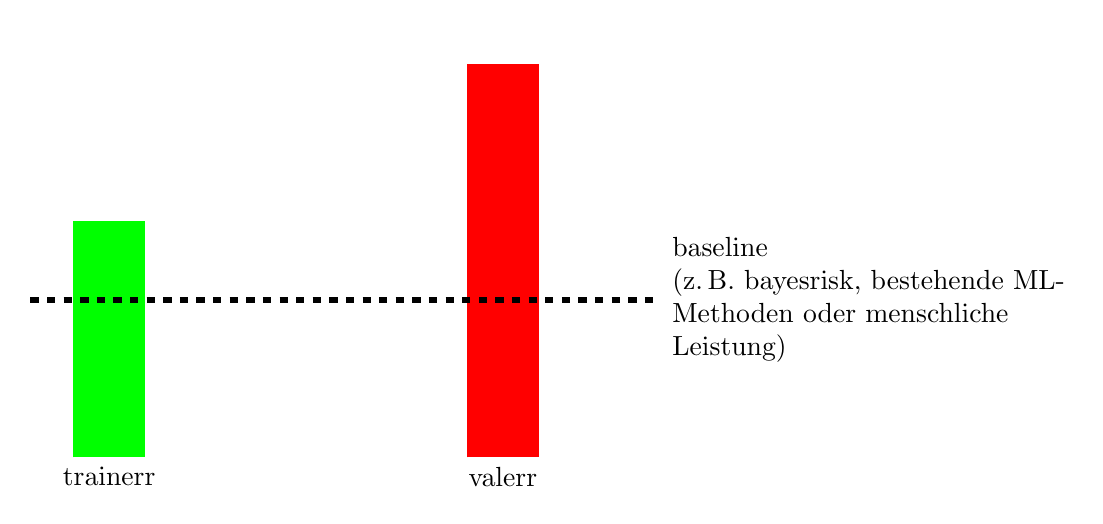
\begin{tikzpicture}[ycomb]
            \draw[color=green,line width=26pt]
            plot coordinates{(0,3)};
            \node [below] at (0,0) {\gls{trainerr}} ; 
            \draw[color=red,line width=26pt]
            plot coordinates{(5,5)};
            \node [below] at (5,0) {\gls{valerr}} ; 
            \draw[dashed,line width=2] (-1,2) -- (7,2) node[right,text width=5cm]{\gls{baseline} \\ (z.\,B. \gls{bayesrisk}, bestehende ML-Methoden oder menschliche Leistung)};
        \end{tikzpicture}
    \end{center}
    \caption{Diagnose einer \gls{erm}-basierten Methode durch Vergleich von \gls{trainerr} und \gls{valerr}. 
    Idealerweise liegen beide Werte auf dem Niveau der \gls{baseline}.\label{fig_diagnosis_dict}}
    \end{figure}
    Siehe auch: \gls{validation}, \gls{kfoldcv}, \gls{generalization}, \gls{baseline}.},
    first={Diagnose},
    text={Diagnose},
	plural={Diagnosen}
}



\newglossaryentry{ml}
{name={Maschinelles Lernen (ML)},
	description={ML\index{machine learning (ML)} zielt darauf ab, ein  \gls{label} anhand der \glspl{feature} eines
		\gls{datapoint} es vorherzusagen. 
		ML-Methoden erreichen dies, indem sie eine \gls{hypothesis aus einem \gls{hypospace} (oder  \gls{model})
			durch Minimierung einer \gls{lossfunc}\cite{MLBasics},  \cite{HastieWainwrightBook} erlernen.
			Eine präzise Formulierung dieses Prinzips ist die \gls{erm}.Verschieden ML-Methoden ergeben sich aus verschiedenen 
			Designentscheidungen für \glspl{datapoint}  {d.h. deren \glspl{features und \glspl{label} }, 
				das \gls{model} und die \gls{lossfunc} \cite[Ch. 3]{MLBasics}.},
	first={Maschinelles Lernen (ML)},text={ML}
} 


\newglossaryentry{reinforcementlearning}
{name={reinforcement learning (RL)},
	description={
	RL\index{reinforcement learning (RL)} refers to a \gls{onlinelearning} setting where 
	we can only evaluate the usefulness of a single \gls{hypothesis} (i.e., a choice of \gls{model} \glspl{parameter}) 
	at each time step $\timeidx$. In particular, RL methods apply the current \gls{hypothesis} 
	$\hypothesis^{(\timeidx)}$ to the \gls{featurevec} $\featurevec^{(\timeidx)}$ of the 
	newly received \gls{datapoint}. The usefulness of the resulting \gls{prediction} 
	$\hypothesis^{(\timeidx)}(\featurevec^{(\timeidx)})$ is quantified by a \gls{reward} 
	signal $\reward^{(\timeidx)}$. 
	\begin{figure}
			\begin{center}
		\begin{tikzpicture}[scale=1]
			\draw[->] (-2, 0) -- (6, 0);
			\node at (6.3, 0) {$\hypothesis$};
	        % loss at time t 
			\draw[thick, blue, domain=0:3, samples=20] plot (\x-3, {-0.2*(\x)^2 + 2});
			\node[anchor=west,yshift=4pt] at (0-3, {-0.2*(0)^2 + 2}) {$-\loss^{(\timeidx)}(\hypothesis)$};
			% Marker and hypothesis label for h^(t)
			\filldraw[blue] (1.5-3, {-0.2*(1.5)^2 + 2}) circle (2pt);
			\node[anchor=north] at (1.5-3, -0.3) {$\hypothesis^{(\timeidx)}$};		
			\draw[dotted] (1.5-3, 0) -- (1.5-3, {-0.2*(1.5)^2 + 2});
			%%% time t+1
			\draw[thick, red, domain=0:5, samples=20, dashed] plot (\x, {-0.15*(\x - 2)^2 + 3});
			\node[anchor=west,yshift=4pt] at (3, {-0.15*(3 - 2)^2 + 3}) {$-\loss^{(\timeidx+1)}(\hypothesis)$};
			\filldraw[red] (2, {-0.15*(2 - 2)^2 + 3}) circle (2pt);
			\node[anchor=north] at (2, -0.3) {$\hypothesis^{(\timeidx+1)}$};
			\draw[dotted] (2, 0) -- (2, {-0.15*(3 - 2)^2 + 3});
			%%% time t+2
			\draw[thick, green!60!black, domain=3:5, samples=20, dotted] plot (\x+2, {-0.1*(\x - 4)^2 + 1.5});
			\node[anchor=west,yshift=4pt] at (4.5+2, {-0.1*(4.5 - 4)^2 + 1.5}) {$-\loss^{(\timeidx+2)}(\hypothesis)$};
			\filldraw[green!60!black] (3.5+2, {-0.1*(3.5 - 4)^2 + 1.5}) circle (2pt);
			\node[anchor=north] at (3.5+2, -0.3) {$\hypothesis^{(\timeidx+2)}$};
			\draw[dotted] (3.5+2, 0) -- (3.5+2, {-0.1*(3.5 - 4)^2 + 1.5});
		\end{tikzpicture}
		\caption{Three consecutive time steps $\timeidx,\timeidx+1,\timeidx+2$ with corresponding \glspl{lossfunc} $\loss^{(\timeidx)},
		\loss^{(\timeidx+1)}, \loss^{(\timeidx+2)}$. During time step $\timeidx$, a RL method can evaluate the 
		\gls{lossfunc} only for one specific \gls{hypothesis} $\hypothesis^{(\timeidx)}$, resulting in the \gls{reward} 
		signal $\reward^{(\timeidx)}=-\loss^{(\timeidx)}(\hypothesis^{(\timeidx)})$.}
			\end{center}
	\end{figure}
	In general, the \gls{reward} depends also on the 
	previous \glspl{prediction} $\hypothesis^{(\timeidx')}\big(\featurevec^{(\timeidx')}\big)$ 
	for $\timeidx' < \timeidx$. The goal of RL is to learn $\hypothesis^{(\timeidx)}$, for 
	each time step $\timeidx$, such that the (possibly discounted) cumulative \gls{reward} 
	is maximized \cite{MLBasics}, \cite{SuttonEd2}.
		\\
		See also: \gls{lossfunc}, \gls{reward}, \gls{ml}.},
	first={reinforcement learning (RL)},
	text={RL}
}

\newglossaryentry{featlearn}
{name={Merkmalslernen},
	description={Betrachten wir eine  \gls{ml} Anwendung mit  \glspl{datapoint} die durch rohe  \glspl{feature} $\featurevec \in \featurespace$ beschrieben 
		werden. \Gls{feature}lernen \index{feature learning} bezeichnet die Aufgabe, eine Abbildung
		$$\featuremapvec: \featurespace \rightarrow \featurespace': \featurevec \mapsto \featurevec'$$ 
		zu lernen, welche rohe \glspl{feature} $\featurevec \in \featurespace$ eines \gls{datapoint}es einliest 
		und neue \glspl{feature} $\featurevec' \in \featurespace'$ aus einem neuen \gls{featurespace} 
		$\featurespace'$ erzeugt. Verschiedene Methoden des \gls{feature}slernens ergeben sich aus unterschiedlichen 
		Gestaltungsentscheidungen für $\featurespace,\featurespace'$,  einem \gls{hypospace} $\hypospace$ möglicher Abbildungen $\featuremapvec$
		sowie einem quantitativen Maß für die Nützlichkeit einer bestimmten Abbildung  $\featuremapvec \in \hypospace$.
		Ein Beispiel ist \gls{pca}, wobei gilt: 
		$\featurespace \defeq \mathbb{R}^{\dimlocalmodel}$, $\featurespace' \defeq \mathbb{R}^{\dimlocalmodel'}$ 
		mit $\dimlocalmodel' < \dimlocalmodel$, und ein \gls{hypospace}
		$$\hypospace\defeq \big\{ \featuremapvec: \mathbb{R}^{\dimlocalmodel}
		\!\rightarrow\! \mathbb{R}^{\dimlocalmodel'}\!:\!\featurevec'\!\defeq\!\mF \featurevec \mbox{ mit } \mF \!\in\! \mathbb{R}^{\dimlocalmodel' \times \dimlocalmodel} \big\}.$$
		\Gls{pca} bewertet die Nützlichkeit einer bestimmten Abbildung $\featuremapvec(\featurevec)= \mF \featurevec$ 
		durch den \gls{minimalen} linearen Rekonstruktionsfehler auf einem \gls{dataset}, also
		$$\min_{\mG \in \mathbb{R}^{\dimlocalmodel \!\!\!\times \dimlocalmodel'}} \sum_{\sampleidx=1}^{\samplesize} \normgeneric{\mG \mF \featurevec^{(\sampleidx)} - \featurevec^{(\sampleidx)}}{2}^{2}.$$ 
			\\ 
	
	first={Merkmalslernen},text={Merkmalslernen}
} 

\newglossaryentry{autoencoder}{
    name={Autoencoder},
    description={Ein Autoencoder\index{autoencoder} ist eine \gls{ml}-Methode, die gleichzeitig 
        einen Encoder-\gls{map} $\hypothesis \in \hypospace$ und einen Decoder-\gls{map} 
        $\hypothesis^{*} \in \hypospace^{*}$ lernt. Verschiedene Autoencoder verwenden unterschiedliche 
        \glspl{model} $\hypospace, \hypospace^{*}$, z.\,B. \glspl{ann} mit verschiedenen Architekturen. 
        Der Spezialfall eines Autoencoders, der (vektorwertige) \glspl{linmodel} für 
        $\hypospace$ und $\hypospace^{*}$ verwendet, entspricht der \gls{pca}.
        \begin{figure}[H]
        \centering
        \begin{tikzpicture}[>=Latex, thick, node distance=1.6cm]
        % Nodes
        \node (x) {$\vx$};
        \node[draw, rounded corners, right=of x, inner sep=4pt] (enc) {$\text{Encoder } \hypothesis$};
        \node[right=of enc] (z) {$\vz$};
        \node[draw, rounded corners, right=of z, inner sep=4pt] (dec) {$\text{Decoder } \hypothesis^{*}$};
        \node[right=of dec] (xhat) {$\hat{\featurevec}$};
        % Arrows
        \draw[->] (x) -- (enc);
        \draw[->] (enc) -- node[above] {$\vz=\hypothesis(\featurevec)$} (z);
        \draw[->] (z) -- (dec);
        \draw[->] (dec) -- node[above] {$\hat{\featurevec}=\hypothesis^{*}(\vz)$} (xhat);
        \end{tikzpicture}
        \caption{Autoencoder mit Encoder $\hypothesis$, der $\featurevec \mapsto \vz$ abbildet, 
        und Decoder $\hypothesis^*$, der $\vz \mapsto \hat{\featurevec}$ abbildet.}
        \end{figure}
        Das Training von Encoder und Decoder kann über \gls{erm} erfolgen, unter Verwendung eines 
        \gls{loss}, der die Abweichung der rekonstruierten \gls{featurevec} 
        $\hypothesis^{*}(\hypothesis(\featurevec))$ von den Originaldaten $\featurevec$ misst.
        Siehe auch: \gls{featlearn}, \gls{dimred}.},
    first={Autoencoder},
    text={Autoencoder}
}


\newglossaryentry{vfl}
{name={Vertikales Kollaboratives Lernen (VFL)},
	description={
		VFL\index{vertical federated learning (VFL)} beschreibt  \gls{fl}  Anwendungen bei denen 
		\gls{device}s Zugang zu verschiedenen  \gls{feature}s desselben  \gls{datapoint}es  \cite{VFLChapter} haben. 
		Das zugrunde liegende globale \gls{dataset ist 
		\[
		\dataset^{(\mathrm{global})} \defeq \left\{ \left(\featurevec^{(1)}, \truelabel^{(1)}\right), \ldots, \left(\featurevec^{(\samplesize)}, \truelabel^{(\samplesize)}\right) \right\}.
		\]
		Wir kennzeichnen  $\featurevec^{(\sampleidx)} = \big( \feature^{(\sampleidx)}_{1}, \ldots, \feature^{(\sampleidx)}_{\nrfeatures'} \big)^{T}$, für $\sampleidx=1,\ldots,\samplesize$, 
		als den kompletten  \gls{featurevec}s für die \glspl{datapoint} . Jedes \gls{device} $\nodeidx \in \nodes$ 
		hat Zugang zu nur einem Teilset  $\mathcal{F}^{(\nodeidx)} \subseteq \{1,\ldots,\nrfeatures'\}$ von  \glspl{feature}s, aus dem ein  
		 \gls{localdataset}  $\localdataset{\nodeidx}$ resultiert mit  \glspl{featurevec}
		\[
		\featurevec^{(\nodeidx,\sampleidx)} = \big( \feature^{(\sampleidx)}_{\featureidx_{1}}, \ldots, \feature^{(\sampleidx)}_{\featureidx_{\nrfeatures}} \big)^{T}.
		\]
		Einige  \glspl{device} können auch Zugang zu den \glspl{label} $\truelabel^{(\sampleidx)}$, for $\sampleidx=1,\ldots,\samplesize$, des globalen \gls{dataset}s haben. Eine potentielle Anwendung für \gls{vfl} sind Kollaborationen zwischen verschiedenen Gesundheitsdienstleistern. 
		Jeder Dienstleister sammelt bestimmte Messungen wie Blutwerte, Elektrokardiographien und Röntgenaufnahmen der Lunge für den selben Patienten. 
		Einer weitere Anwendung ist ein nationales Sozialversicherungssystem, in dem Gesundheitsdaten, finanzielle Indikatoren, Verbraucherverhalten und Mobilitäts\glspl{data} von verschiedenen Institutionen gesammelt werden.  \gls{vfl} ermöglicht gemeinsames lernen zwischen diesen Parteien und gleichzeitig ein genau definiertes Maß an \gls{privprot}.
		
		\begin{figure}[htbp]
			\begin{center}
				\begin{tikzpicture}[every node/.style={anchor=base}]
					% --- Coordinate definitions ---
					\def\colX{0}
					\def\colY{1.6}
					\def\colZ{3.2}
					\def\colD{4.8}
					\def\colLabel{6.4} 
					\def\rowOne{0}
					\def\rowTwo{-1.2}
					\def\rowThree{-2.4}
					\def\rowFour{-3.6}
					% Manually place matrix entries
					\foreach \i/\label in {1/1, 2/2, 4/\samplesize} {
						\pgfmathsetmacro{\y}{-1.2*(\i-1)}
						\node (x\i1) at (0,\y) {$x^{(\label)}_{1}$};
						\node (x\i2) at (1.6,\y) {$x^{(\label)}_{2}$};
						\node (dots\i) at (3.2,\y) {$\cdots$};
						\node (x\i3) at (4.8,\y) {$x^{(\label)}_{\dimlocalmodel}$};
						\node (y\i) at (6.4,\y) {$\truelabel^{(\label)}$};
					}
					% Outer rectangle for the full dataset
					\draw[dashed, rounded corners, thick]
					(-0.6,0.6) rectangle (6.9,-4.2);
					\node at (3.1,0.9) {$\dataset^{(\mathrm{global})} $};
					% Rectangle for local dataset 1 (e.g., first two features)
					\draw[dashed, rounded corners, thick]
					(-0.9,0.9) rectangle (2.1,-4.0);
					\node at (0.25,1.0) {$\localdataset{1}$};
					% --- Local dataset k (columns 2–3, rows 1–3) ---
					\draw[dashed, rounded corners, thick]
					($( \colZ + 1,,0.9 )$) rectangle
					($( \colLabel + 0.4, -4.5)$);
					\node at ($( \colZ + 0.9,-5 )$) {$\localdataset{\nodeidx}$};
				\end{tikzpicture}
			\end{center}
			\caption{VFL nutzt \glspl{localdataset}  die von  \glspl{datapoint} eines gemeinsamen globalen \gls{dataset}es abgeleitet sind. 
				Die \glspl{localdataset} unterschieden sich in der Wahl der \glspl{feature} die verwendet werden, um die  \glspl{datapoint} zu charakterisieren.
				\label{fig_vertical_FL}}
	\end{figure}},
	first={Vertikales Kollaboratives Lernen (VFL)},text={VFL}
} 

\newglossaryentry{interpretability}{
    name={Interpretierbarkeit},
    description={Eine \gls{ml}-Methode ist für einen menschlichen Benutzer interpretierbar\index{Interpretierbarkeit}, 
        wenn dieser den Entscheidungsprozess der Methode nachvollziehen kann. 
        Eine präzise Definition von Interpretierbarkeit lässt sich über das Konzept der Simulierbarkeit ableiten, 
        d.\,h. die Fähigkeit eines Menschen, das Verhalten des \gls{model} mental zu simulieren 
        \cite{Colin:2022aa, Chen2018, doshi2017towards, hase-bansal-2020-evaluating, Lipton2018}. 
        Konkret gilt: Wenn ein Benutzer eine \gls{ml}-Methode versteht, sollte er die 
        \glspl{prediction} des gelernten \glspl{hypothesis} $\learnthypothesis$ auf einer \gls{testset} 
        antizipieren können. 
        \begin{figure}[H]
            \begin{center} 
            \begin{tikzpicture}[x=1.5cm, y=1cm]
                % Achsen
                \draw[->, very thick] (0,0.5) -- (7.7,0.5) node[below, xshift=-1cm] {$\feature$};
                \draw[->, very thick] (0.5,0) -- (0.5,4.2) node[above] {$\truelabel$};
                % Interpretierbares Modell
                \draw[color=black, thick, dashed, domain=-0.5:7.2, variable=\x] plot ({\x},{0.4*\x + 2.0});
                % Nicht interpretierbares Modell
                \draw[color=black, thick, dashed, domain=4:7.2, variable=\x] plot ({\x},{0.4*\x + 2.0-(\x-4)*0.5});
                \node[above] at (7.2, 0.4*7.2 + 2.0) {$\learnthypothesis(\feature)$};
                \node[above] at (7.2, 0.4*7.2 + 2.0 - 0.5*(7.2 - 4)) {$\learnthypothesis'(\feature)$};
                % Trainingsdatenpunkte
                \foreach \x/\y/\c/\s in {1.2/1.0/blue/6, 1.4/1.0/blue/6, 1.7/1.0/blue/6,
                                         2.2/3.9/blue/12, 2.6/4.2/blue/12, 3.0/4.4/blue/12}{
                    \node[fill=\c, circle, draw, minimum size=\s pt, scale=0.6] at (\x,\y) {};
                    \draw[<->, >={Latex[width=2mm,length=4mm]}, color=\c, thick] (\x, {0.4*\x + 2.0}) -- (\x,\y);
                }
                % Testdatenpunkte
                \foreach \x/\y/\c/\s in {5.7/2.6/red/12, 5.9/2.6/red/12, 6.2/2.6/red/12}{
                    \node[fill=\c, circle, draw, minimum size=\s pt, scale=0.6] at (\x, {0.4*\x + 2.0}) {};
                }
                % Legende
                \draw[fill=blue] (4.2, 1.7) circle (0.1cm) node [black,xshift=0.2cm,anchor=west] {\gls{trainset} $\dataset$};
                \draw[fill=red]  (4.2, 1.2) circle (0.1cm) node [black,xshift=0.2cm,anchor=west] {\gls{testset} $\dataset'$};
            \end{tikzpicture}
            \caption{Interpretierbarkeit eines gelernten \gls{ml}-\gls{model} $\learnthypothesis$ 
            und eines nicht interpretierbaren Modells $\learnthypothesis'$ durch Vergleich der \glspl{prediction} 
            mit pseudo-\glspl{label} eines menschlichen Benutzers für $\dataset'$. 
            \label{fig_aug_simulatability_dict}}
            \end{center}
        \end{figure}
        Interpretierbarkeit ist eng verwandt mit \gls{explainability}, da beide darauf abzielen, 
        \gls{ml}-Methoden für Menschen verständlich zu machen. Während Interpretierbarkeit die Fähigkeit 
        eines Benutzers voraussetzt, \glspl{prediction} auf beliebigen \gls{testset} vorherzusagen, 
        unterstützt \gls{explainability} den Benutzer durch externe \glspl{explanation}, 
        wie z.\,B. Saliency-\glspl{map} oder Referenzbeispiele aus dem \gls{trainset}, 
        um einzelne \glspl{prediction} nachvollziehen zu können.
        Siehe auch: \gls{explainability}, \gls{trustAI}, \gls{regularization}, \gls{lime}.},
    first={Interpretierbarkeit},
    text={interpretability}
}




\newglossaryentry{multitask learning}
{name={Multitask Lernen },description=
	{Multitask Lernen \index{multitask learning} zielt darauf ab, Beziehungen  zwischen verschiedenen  \glspl{learningtask} auszunutzen.
	Betrachten wir zwei  \glspl{learningtask} die vom gleichen  \gls{dataset} bestehend aus webcam Bildaufnahmen, gewonnen werden. 
	Die erste  \gls{learningtask} besteht darin, die Anwesenheit eines Menschen zu bestimmen, die zweite Aufgabe hingegen ist die Anwesenheit 
	eines Autos zu bestimmen. Es kann sinnvol sein, die gleiche  \gls{deepnet} Struktur für beide  \glspl{learningtask}  zu verwenden und nur die \gls{weights} 
	der finalen Ausgabeschicht unterschiedlich zu gestalten. 
	
		 Consider two \gls{learningtask}s obtained from the  \gls{deepnet} 
		same \gls{dataset} of webcam snapshots. The first task is to predict the presence 
		of a human, while the second task is to predict the presence of a car. It might be useful 
		to use the same \gls{deepnet} structure for both tasks and only allow the \gls{weights} of 
		the final output layer to be different.},
	first={Multitask Lernen},text={Multitask Lernen}
}

\newglossaryentry{learningtask}
{name={Lernaufgabe},description=
	{Consider\index{learning task} a \gls{dataset} $\dataset$ constituted by several \gls{datapoint}s, each of them 
		characterized by \gls{feature}s $\featurevec$. For example, the \gls{dataset} $\dataset$ 
		might be constituted by the images of a particular database. Sometimes it might be useful 
		to represent a \gls{dataset} $\dataset$, along with the choice of \gls{feature}s, by a \gls{probdist} $p(\featurevec)$. 
		A learning task associated with $\dataset$ consists of a specific 
		choice for the \gls{label} of a \gls{datapoint} and the corresponding \gls{labelspace}. 
		Given a choice for the \gls{lossfunc} and \gls{model}, a learning task gives rise to an 
		instance of \gls{erm}. Thus, we could define a learning task also via an instance of \gls{erm}, i.e., 
		via an \gls{objfunc}. Note that, for the same \gls{dataset}, we obtain different learning tasks by using 
		different choices for the \gls{feature}s and \gls{label} of a \gls{datapoint}. These learning 
		tasks are related, as they are based on the same \gls{dataset}, and solving them jointly 
		(via \gls{multitask learning} methods) is typically preferable over solving them separately \cite{Caruana:1997wk}, \cite{JungGaphLassoSPL}, \cite{CSGraphSelJournal}.},
	first={Lernaufgabe},text={{name={Lernaufgabe},description=
			{Betrachten wir eine \index{learning task}  mit einem  \gls{dataset} $\dataset$ bestehen aus verschiedenen  \glspl{datapoint}n, jeder charakterisiert durch  \glspl{feature}  $\featurevec$. 
				Der \gls{dataset} $\dataset$  könnte beispielsweise aus Bildern aus einer bestimmten Datenbank bestehen. 
				Manchmal kann es hier hilfreich sein, den  \gls{dataset} $\dataset$ zusammen mit der Wahl der  \glspl{feature} durch eine  \gls{probdist} $p(\featurevec)$ zu repräsentieren. 
				Eine Lernaufgabe, die mit  $\dataset$ assoziiert ist, besteht aus einer spezifischen Wahl des \gls{label}s für einen \gls{datapoint}, sowie des zugehörigen  \gls{labelspace}es. 
				Bei gegebener Wahl der  \gls{lossfunc} und des \gls{model}s, ergibt sich aus einer Lernaufgabe eine Instanz 
				von \gls{erm}. Daher kann man eine Lernaufgabe auch direkt durch eine Instanz von \gls{erm}, 
				d. h. über eine \gls{objfunc}, definieren.
				
				Beachte, dass sich aus demselben \gls{dataset} unterschiedliche Lernaufgaben ergeben, wenn man 
				unterschiedliche \gls{feature}s und \gls{label} für einen \gls{datapoint} wählt. 
				Diese Lernaufgaben sind miteinander verwandt, da sie auf demselben \gls{dataset} basieren. 
				Es ist in der Regel vorteilhaft, sie gemeinsam (z. B. durch \gls{multitask learning}-Methoden) 
				zu lösen, anstatt sie getrennt zu behandeln \cite{Caruana:1997wk}, \cite{JungGaphLassoSPL}, \cite{CSGraphSelJournal}.
				},
				first={Lernaufgabe},
				text={Lernaufgabe},

			}
		
		
		\newglossaryentry{explainability}
			{name={Erklärbarkeit},description=
				{Wir \index{explainability} definierien die subjektive Erklärbarkeit einer \gls{ml}- Methode als Maß für den Grad der 
						Simulierbarkeit \cite{Colin:2022aa} der von einem \gls{ml}- System gelieferten \glspl{prediction} fü einen menschlichen Nutzer. Quantiative Maße der subjektiven Erllärbarkeit eines trainierten \gls{model}s können konstruiert werden, in dem man dessen 
						\glspl{prediction} mit den \glspl{prediction} vergleicht, die von einem Nutzer durch ein \gls{testset} bereitgestellt werden \cite{Colin:2022aa}, \cite{Zhang:2024aa}. 
						Alternativ können wir 
						Alternatively, we can use \glspl{probmodel} für  \gls{data} verwednen und die Erklärbarkeit eines trainierten \gls{ml} 
						\gls{model}s über die konditionale (bzw. differentielle) Entropie seiner  \glspl{prediction}, bei gegebenen \glspl{prediction} der Nutzer messen \cite{JunXML2020}, \cite{Chen2018}. 
					},
					first={Erklärbarkeit},text={Erklärbarkeit}
				}
				
				
				\newglossaryentry{lime}
				{name={lokale interpretierbare modellunabhängige Erklärungen (LIME)},
					description={
						Betrachten wir \index{local interpretable model-agnostic explanations (LIME)} eine trainiertes  \gls{model} (oder erlernte \gls{hypothesis}) $\widehat{\hypothesis} \in \hypospace$, die den \gls{featurevec} eines  \gls{datapoint}es auf die \gls{prediction} $\widehat{\truelabel}= \widehat{\hypothesis}$ abbildet. 
						Lokale interåretierbare \gls{model}-agnostische \glspl{explanation} sind eine Technik zur Erklärung des Verhalten von $\widehat{\hypothesis}$ 
						lokal um einen \gls{datapoint} mit \gls{featurevec} $\featurevec^{(0)}$ \cite{Ribeiro2016}. 
						Diese Annäherung kann durch eine Instanz von \gls{erm} mit sorgfältig gewähltem \gls{trainset} gewonnen werden. 
						Insbesondere besteht das \gls{trainset} aus \glspl{datapoint} mit \gls{featurevec} $\featurevec$, die nahe bei 
						$\featurevec^{(0)}$ liegen und  aus dem (Pseudo-)Label $\widehat{\hypothesis}(\featurevec)$. 
						Beachte, dass für die Annäherung ein anderes \gls{model} $\hypospace'$ verwendet werden kann als für das Originalmodell $\hypospace$. 
						Zum Beispiel kann ein \gls{decisiontree} verwendet werden, um lokal ein \gls{deepnet} zu approximieren. 
						Eine weitere häufig verwendete Wahl für $\hypospace'$ ist das \gls{linmodel}.
					
						\begin{figure}[H]
							\begin{center}
								\begin{tikzpicture}
									\begin{axis}[
										axis lines=middle,
										xlabel={$\featurevec$},
										ylabel={$\truelabel$},
										xtick=\empty,
										ytick=\empty,
										xmin=0, xmax=6,
										ymin=0, ymax=6,
										domain=0:6,
										samples=100,
										width=10cm,
										height=6cm,
										clip=false
										]
										% Non-linear model h(x)
										\addplot[blue, thick, domain=0:6] {2 + sin(deg(x))} node[pos=0.85, above right,yshift=3pt] {$\widehat{\hypothesis}(\featurevec)$};
										% Feature value x0
										\addplot[dashed, gray] coordinates {(3,0) (3,6)};
										% Piecewise constant local approximation g(x)
										\addplot[red, thick, domain=2.5:3.5] {2 + sin(deg(3))} node[pos=0.9, above] {$g(\featurevec)$};
										% Optional: mark the point of approximation
										\addplot[mark=*] coordinates {(3, {2 + sin(deg(3))})};
										\node at (axis cs:3,-0.3) {$\featurevec^{(0)}$};
									\end{axis}
								\end{tikzpicture}
							\end{center}
							\caption{{Zur Erklärung eines trainierten \gls{model} $\widehat{\hypothesis} \in \hypospace$ 
									in der Umgebung eines gegebenen \gls{featurevec} $\featurevec^{(0)}$ kann eine lokale Approximation $g \in \hypospace'$ verwendet werden.}
							\label{fig_lime}
					\end{figure}},
					first={LIME},text={LIME}
				}
				
\newglossaryentry{linmodel}{
    name={lineares Modell}, 
    description={Betrachten wir\index{lineares Modell} eine \gls{ml}-Anwendung mit \glspl{datapoint}, 
        die jeweils durch einen numerischen \gls{featurevec} $\featurevec \in \mathbb{R}^{\nrfeatures}$ 
        dargestellt werden. Ein lineares \gls{model} definiert einen \gls{hypospace}, der alle reellen 
        \glspl{linearmap} von $\mathbb{R}^{\nrfeatures}$ nach $\mathbb{R}$ umfasst, sodass
        \begin{equation}
            \nonumber
            \label{equ_def_lin_model_hypspace_dict}
            \linmodel{\nrfeatures} \defeq \left\{ \hypothesis: \mathbb{R}^{\nrfeatures} \rightarrow \mathbb{R} \mid \hypothesis(\featurevec) = \weights^{\top} \featurevec \text{ für ein } \weights \in \mathbb{R}^{\nrfeatures} \right\}.
        \end{equation}
        Jeder Wert von $\nrfeatures$ definiert einen unterschiedlichen \gls{hypospace}, entsprechend der Anzahl 
        der \glspl{feature}, die zur Berechnung der \gls{prediction} $\hypothesis(\featurevec)$ verwendet werden. 
        Die Wahl von $\nrfeatures$ wird oft nicht nur durch \gls{compasp} (z. B. weniger Merkmale reduzieren den Rechenaufwand) 
        und \gls{statasp} (z. B. mehr Merkmale verringern typischerweise \gls{bias} und \gls{risk}), sondern auch durch 
        \gls{interpretability} geleitet. Ein lineares \gls{model} mit wenigen, gut gewählten \glspl{feature} gilt im Allgemeinen 
        als besser interpretierbar \cite{rudin2019stop, Ribeiro2016}.
        Lineare \glspl{model} sind attraktiv, da sie typischerweise mit skalierbaren \gls{convex}-\glspl{optmethod} 
        trainiert werden können \cite{hastie01statisticallearning, BertsekasNonLinProgr}. 
        Zudem erlauben lineare \glspl{model} oft eine rigorose statistische Analyse, einschließlich fundamentaler 
        Grenzen für das \gls{minimum} erreichbarer \gls{risk} \cite{Wain2019}. Sie sind auch nützlich zur Analyse 
        komplexerer, nichtlinearer \glspl{model} wie \glspl{ann}. Zum Beispiel kann ein \gls{deepnet} als 
        Komposition einer \gls{featuremap}—implementiert durch Eingabe- und versteckte \glspl{layer}—und eines 
        linearen \gls{model} in der Ausgabeschicht betrachtet werden. Ähnlich kann ein \gls{decisiontree} 
        als Anwendung einer One-Hot-kodierten \gls{featuremap} basierend auf \glspl{decisionregion} 
        interpretiert werden, gefolgt von einem linearen \gls{model}, das jeder Region eine \gls{prediction} zuordnet.
        Allgemeiner kann jedes trainierte \gls{model} $\learnthypothesis \in \hypospace$, das bei einem Punkt 
        $\featurevec'$ \gls{differentiable} ist, lokal durch eine \gls{linearmap} $g(\featurevec)$ approximiert werden. 
        Abbildung~\ref{fig_linapprox_dict} zeigt eine solche lokale lineare Approximation, definiert durch den 
        \gls{gradient} $\nabla \learnthypothesis(\featurevec')$. Beachte, dass der \gls{gradient} nur dort definiert 
        ist, wo $\learnthypothesis$ \gls{differentiable} ist.
        Um \gls{robustness} im Kontext von \gls{trustAI} zu gewährleisten, bevorzugt man möglicherweise 
        \glspl{model}, deren zugehörige \gls{map} $\learnthypothesis$ Lipschitz-stetig ist. Ein klassisches Ergebnis 
        der mathematischen Analyse—Rademacher’s Theorem—besagt, dass, wenn $\learnthypothesis$ über einer offenen 
        Menge $\samplespace \subseteq \mathbb{R}^{\nrfeatures}$ Lipschitz-stetig mit Konstante $L$ ist, 
        $\learnthypothesis$ fast überall in $\samplespace$ \gls{differentiable} ist \cite[Th.~3.1]{heinonen2005lectures}.
        \begin{figure}[H]
        \begin{center}
        % TikZ-Figur bleibt unverändert, nur Bildbeschreibung übersetzt
        \caption{
            Ein trainiertes \gls{model} $\learnthypothesis(\featurevec)$, das an einem Punkt $\featurevec'$ 
            \gls{differentiable} ist, kann lokal durch eine \gls{linearmap} $g \in \linmodel{\nrfeatures}$ 
            approximiert werden. Diese lokale Approximation wird durch den \gls{gradient} 
            $\nabla \learnthypothesis(\featurevec')$ bestimmt.}
        \label{fig_linapprox_dict}
        \end{center}
        \end{figure}
        Siehe auch: \gls{model}, \gls{hypospace}, \gls{linearmap}, \gls{interpretability}, \gls{lime}.}, 
    first={lineares Modell},
    plural={lineare Modelle},
    firstplural={lineare Modelle}, 
    text={linear model}
}



\newglossaryentry{gradstep}{name={Gradientenschritt},
	description= Gegeben sei eine \gls{differentiable} reellwertiger Funktion$f(\cdot): \mathbb{R}^{\nrfeatures} \rightarrow \mathbb{R}$  und ein Vektor 
		$\weights \in \mathbb{R}^{\nrfeatures}$. Der  \gls{gradient}enschritt \index{gradient step} aktualisiert  $\weights$ indem der skalierte negative \gls{gradient} $\nabla f(\weights)$ addiert wird.(siehe Fig. \ref{fig_basic_GD_step_single_dict})
	
		\begin{equation}
			\label{equ_def_gd_basic_dict} 
			\widehat{\weights}  \defeq \weights - \lrate \nabla f(\weights).
		\end{equation} 
		 Mathematisch ist der  \gls{gradient}enschritt ein (typischerweise nichtlinearer) Operator  $\mathcal{T}^{(f,\lrate)}$ der durch die Funktion $f$
		 und die  \gls{stepsize} $\lrate$ parametrisiert wird. 
	
		\begin{figure}[H]
			\begin{center}
				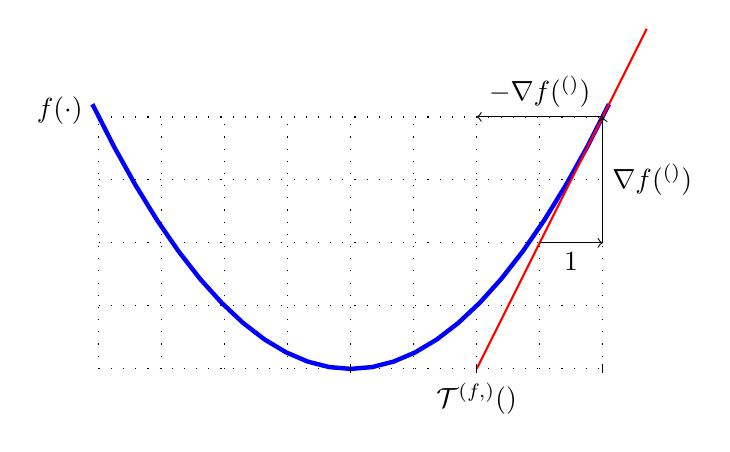
\begin{tikzpicture}[scale=0.8]
					\draw[loosely dotted] (-4,0) grid (4,4);
					\draw[blue, ultra thick, domain=-4.1:4.1] plot (\x,  {(1/4)*\x*\x});
					\draw[red, thick, domain=2:4.7] plot (\x,  {2*\x - 4});
					\draw[<-] (4,4) -- node[right] {$\nabla f(\weights^{(\itercntr)})$} (4,2);
					\draw[->] (4,4) -- node[above] {$-\lrate \nabla f(\weights^{(\itercntr)})$} (2,4);
					\draw[<-] (4,2) -- node[below] {$1$} (3,2) ;
					%\draw[->] (-4.25,0) -- (4.25,0) node[right] {$a$};
					\node[left] at (-4.1, 4.1) {$f(\cdot)$}; 
					\draw[shift={(0,0)}] (0pt,2pt) -- (0pt,-2pt) node[below] {$\overline{\weights}$};
					\draw[shift={(4,0)}] (0pt,2pt) -- (0pt,-2pt) node[below] {$\weights$};
					\draw[shift={(2,0)}] (0pt,2pt) -- (0pt,-2pt) node[below] {$\mathcal{T}^{(f,\lrate)}(\weights)$};
				\end{tikzpicture}
			\end{center}
			\caption{Der grundlegende \gls{gradient} enschjritt \eqref{equ_def_gd_basic_dict}  bildet einen gegebenen Vektro  $\weights$ 
				auf den aktualisierten Vektor $\weights'$ ab. Er definiert einen Operator,
				$\mathcal{T}^{(f,\lrate)}(\cdot): \mathbb{R}^{\nrfeatures} \rightarrow \mathbb{R}^{\nrfeatures}:
				\weights \mapsto \widehat{\weights}$.}
			\label{fig_basic_GD_step_single_dict}
		\end{figure}
		Beachte das der  \gls{gradient}enschritt \eqref{equ_def_gd_basic_dict} lokal optimisiert - in einer \gls{neighborhood}, deren Größe durch die  \gls{stepsize} $\lrate$, eine lineare Annäherung an die Funktion $f(\cdot)$ bestimmt wird.  
		Eine naheliegende  \gls{Verallgemeinerung} 
		von \eqref{equ_def_gd_basic_dict} besteht darin, die Funktion selbst, statt der linearen Annäherung,  lokal zu optimieren, sodass:
		
		\begin{align} 
			\label{equ_approx_gd_step_dict}
			\widehat{\weights} = \argmin_{\weights' \in \mathbb{R}^{\dimlocalmodel}} f(\weights')\!+\!(1/\lrate)\normgeneric{\weights-\weights'}{2}^2. 
		\end{align}
		Wir verwenden absichtlich das gleiche Symbol $\lrate$ wie in \eqref{equ_def_gd_basic_dict}, 
		da auch hier gilt: Je größer $\lrate$, desto größer typischerweise der Fortschritt hin zu 
		einem kleineren Funktionswert $f(\widehat{\weights})$. Ähnlich wie der Gradientenschritt 
		\eqref{equ_def_gd_basic_dict} definiert auch die Aktualisierung \eqref{equ_approx_gd_step_dict} 
		einen (typischerweise nichtlinearen) Operator, der durch die Funktion $f(\cdot)$ und den Parameter 
		$\lrate$ bestimmt ist. Für eine \gls{konvexe} Funktion $f(\cdot)$ ist dieser Operator auch als 
		\gls{proxop} der Funktion bekannt \cite{ProximalMethods}.
		},
		first={Gradientenschritt},text={Gradientenschritt},plural={Gradientenschritte}
}

\newglossaryentry{operator} 
{
    name={Operator}, 
    description={Ein\index{Operator} Operator ist eine \gls{function}, 
        deren \gls{domain} und \gls{co-domain} eine spezifische mathematische Struktur aufweisen, 
        wie z. B. ein \gls{vectorspace}, \gls{hilbertspace} oder \gls{metricspace} \cite{Bauschke:2017,DunfordSchwartz1988}. 
        Viele \gls{ml}-Methoden arbeiten mit Operatoren, deren \gls{domain} und \gls{co-domain} 
        ein \gls{euclidspace} sind.
        \\
        Siehe auch: \gls{vectorspace}, \gls{function}, \gls{hilbertspace}.},
    first={Operator},
    type=math, 
    plural={Operatoren},
    firstplural={Operatoren},
    text={Operator}
}


\newglossaryentry{contractop}
{name={contraction operator},
	description={An\index{contraction operator} operator $\fixedpointop: \mathbb{R}^{\nrfeatures} \rightarrow \mathbb{R}^{\nrfeatures}$
		is a contraction if, for some $\contractfac \in [0,1)$,
		\begin{equation} 
			\nonumber
			\normgeneric{ \fixedpointop \weights\!-\!\fixedpointop \weights'}{2}  \leq  \contractfac	\normgeneric{\weights\!-\!\weights'}{2} \mbox{ holds for any } \weights,\weights' \in \mathbb{R}^{\nrfeatures}.
		\end{equation}
	},
	first={contraction operator},
	text={contraction operator}, 
	firstplural={contraction operators}, 
	plural={contraction operators}
}


\newglossaryentry{proxop}
{name={Proximaloperator},
	description={Gegeben sei \index{proximal operator} eine \gls{convex}e Funktion $f(\weights')$. Wir definieren ihren Proximal Operator gemäß \cite{ProximalMethods}, \cite{Bauschke:2017} als: 
		$$\proximityop{f(\cdot)}{\weights}{\rho}\defeq \argmin_{\weights' \in \mathbb{R}^{\dimlocalmodel}} \bigg[ f(\weights')\!+\!(\rho/2) \normgeneric{\weights- \weights'}{2}^{2}\bigg] \mbox{ mit } \rho > 0. $$ 
		Wie in Fig. \ref{fig_proxoperator_opt_dict}  illustriert, entspricht die Auswertung des Proximaloperators der Minimierung einer penalisierten Variante von $f(\weights')$. Der Strafterm ist der skalierte quadratische euklidische Abstand zu einem gegebenen Vektor $\weights$ (welcher der Eingabewert des Proximaloperators ist).
	
		%\Gls{convex} functions for which the proximal operator can be computed efficiently 
		%is sometimes referred to as \emph{proximable} or \emph{simple} \cite{Condat2013}. 
		Der Proximaloperator kann als eine \gls{generalization} des e \gls{gradstep}s interpretiert werden, der für eine \gls{smooth} \gls{convex}e Funktion  $f(\weights') $ definiert ist. Tatsächlich entspricht ein
		\gls{gradstep} mit \gls{stepsize} $\lrate$ am momentanen Vektor r $\weights$ der Anwendung des Proximaloperators der Funktion 
		 $\tilde{f}(\weights')= \big( \nabla f(\weights)\big)^{T} (\weights'-\weights)$ 
		mit $\rho=1/\lrate$.
		\begin{figure}[H]
			\begin{center}
				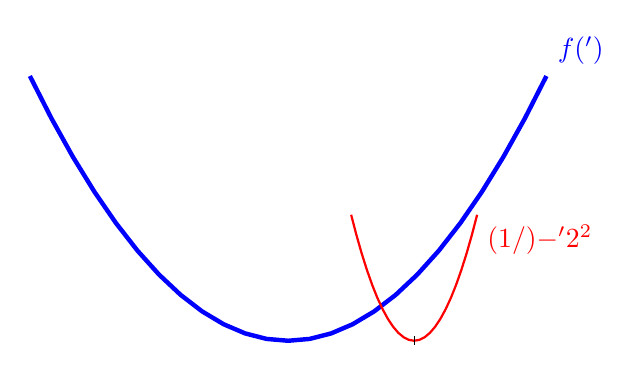
\begin{tikzpicture}[scale=0.8]
					% Original quadratic function
					\draw[blue, ultra thick, domain=-4.1:4.1] plot (\x, {(1/4)*\x*\x}) node[above right] {$f(\weights')$};		
					% Quadratic function with larger curvature, centered at w = 2
					\draw[red, thick, domain=1:3] plot (\x, {2*(\x - 2)*(\x - 2)}) node[below right] {$(1/\lrate)\normgeneric{\weights-\weights'}{2}^{2}$};
					% Axes
					% Minimum point of second curve
					\draw[shift={(2,0)}] (0pt,2pt) -- (0pt,-2pt) node[below] {$\weights$};
					%\node at (2,0.5) [anchor=north] {$\weights$};
				\end{tikzpicture}
			\end{center}
			\caption{A generalized \gls{gradstep} updates a vector $\weights$ by minimizing a penalized version 
				of the function $f(\cdot)$. The penalty term is the scaled squared Euclidean distance between the optimization 
				variable $\weights'$ and the given vector $\weights$.	\label{fig_proxoperator_opt_dict}}
		\end{figure}
	},first={proximal operator},text={proximal operator}}
}

	
\newglossaryentry{proximable}
{
    name={proximierbar},
    description={Eine\index{proximierbar} \gls{convex} \gls{function}, für die der \gls{proxop} effizient berechnet werden kann, 
        wird manchmal als proximierbar oder einfach bezeichnet \cite{Condat2013}.
        \\
        Siehe auch: \gls{convex}, \gls{function}, \gls{proxop}.},
    first={proximierbar},
    text={proximierbar}
}


\newglossaryentry{connected}
{
    name={zusammenhängend}, 
    description={Ein\index{zusammenhängend} \gls{undirectedgraph} $\graph=\pair{\nodes}{\edges}$ 
        ist zusammenhängend, wenn für jede nicht-leere Teilmenge $\nodes' \subset \nodes$ 
        mindestens eine Kante existiert, die einen Knoten in $\nodes'$ mit einem Knoten in $\nodes \setminus \nodes'$ verbindet.
        \begin{figure}[H]
        \centering
        \begin{tikzpicture}
        % Linkes Diagramm (nicht zusammenhängend)
        \node[circle, fill=black, inner sep=1.5pt, label=above:{1}] (A1) at (0, 1.5) {};
        \node[above=0.5cm of A1, align=center] {nicht zusammenhängend};
        \node[circle, fill=black, inner sep=1.5pt, label=below right:{2}] (B1) [below right=0.8cm and 0.5cm of A1] {};
        \node[circle, fill=black, inner sep=1.5pt, label=below left:{3}] (C1) [below left=0.8cm and 0.5cm of A1] {};
        \draw [line width=1 pt]  (A1) -- (B1);
        % Rechtes Diagramm (zusammenhängend)
        \begin{scope}[xshift=3.5cm]
            \node[circle, fill=black, inner sep=1.5pt, label=above:{1}] (A2) at (0, 1.5) {};
            \node[above=0.5cm of A2, align=center] {zusammenhängend};
            \node[circle, fill=black, inner sep=1.5pt, label=below right:{2}] (B2) [below right=0.8cm and 0.5cm of A2] {};
            \node[circle, fill=black, inner sep=1.5pt, label=below left:{3}] (C2) [below left=0.8cm and 0.5cm of A2] {};
            \draw [line width=1 pt]  (A2) -- (B2);
            \draw [line width=1 pt]  (B2) -- (C2);
        \end{scope}
        \end{tikzpicture}
        \end{figure} 
        Siehe auch: \gls{undirectedgraph}, \gls{algconn}.}, 
    type=math, 
    first={zusammenhängend},
    text={zusammenhängend}
}


\newglossaryentry{mvndist}
{
    name={multivariate Normalverteilung}, 
    description={Die\index{multivariate Normalverteilung} multivariate Normalverteilung, 
        die mit $\mvnormal{\meanvecgeneric}{\covmtxgeneric}$ bezeichnet wird, ist ein fundamentales 
        \gls{probmodel} für numerische \glspl{featurevec} fester Dimension $\nrfeatures$. 
        Sie definiert eine Familie von \glspl{probdist} über \gls{vector}-wertige \glspl{rv} 
        $\featurevec \in \mathbb{R}^{\nrfeatures}$~\cite{BertsekasProb,GrayProbBook,Lapidoth09}. 
        Jede Verteilung aus dieser Familie wird vollständig durch ihren \gls{mean}-\gls{vector} 
        $\meanvecgeneric \in \mathbb{R}^{\nrfeatures}$ und ihre \gls{covmtx} 
        $\covmtxgeneric \in \mathbb{R}^{\nrfeatures \times \nrfeatures}$ bestimmt. 
        Wenn die \gls{covmtx} $\covmtxgeneric$ invertierbar ist, wird die entsprechende 
        \gls{probdist} durch die folgende \gls{pdf} beschrieben:
        \[
        p(\featurevec) = 
        \frac{1}{\sqrt{(2\pi)^{\nrfeatures} \det\,(\covmtxgeneric)}} 
        \exp\Big[ -\frac{1}{2} 
        (\featurevec - \meanvecgeneric)\,^{T}\, \covmtxgeneric^{-1} 
        (\featurevec - \meanvecgeneric) \Big].
        \]
        Diese \gls{pdf} ist nur definiert, wenn $\covmtxgeneric$ invertierbar ist.
        Allgemeiner gilt für jede \gls{rv} $\featurevec \sim \mvnormal{\meanvecgeneric}{\covmtxgeneric}$ die Darstellung:
        \[
        \featurevec = \mA \vz + \meanvecgeneric,
        \]
        wobei $\vz \sim \mvnormal{\mathbf{0}}{\mathbf{I}}$ ein \gls{stdnormvec} ist und 
        $\mA \in \mathbb{R}^{\nrfeatures \times \nrfeatures}$ die Bedingung $\mA \mA^\top = \covmtxgeneric$ erfüllt. 
        Diese Darstellung bleibt auch gültig, wenn $\covmtxgeneric$ singulär ist, wobei $\mA$ in diesem Fall 
        nicht vollrangig ist~\cite[Ch. 23]{Lapidoth2017}.
        Die Familie der multivariaten Normalverteilungen ist unter \glspl{probmodel} für numerische 
        Größen besonders, insbesondere aus folgenden Gründen. Erstens ist die Familie abgeschlossen unter affinen 
        Transformationen, d.h.,
        \[
        \featurevec \sim \mathcal{N}(\meanvecgeneric,\covmtxgeneric) \implies 
        \mB\featurevec\!+\!\vc \sim \mathcal{N}\big( \mB\meanvecgeneric+\vc,\mB \covmtxgeneric \mB\,^{T} \big). 
        \]
        Zweitens maximiert die \gls{probdist} $\mathcal{N}(\mathbf{0},\covmtxgeneric)$ die 
        \gls{diffentropy} unter allen Verteilungen mit derselben \gls{covmtx} $\covmtxgeneric$~\cite{coverthomas}. 
        \\ 
        Siehe auch: \gls{probmodel}, \gls{probdist}, \gls{stdnormvec}, \gls{diffentropy}, \gls{gaussrv}.}, 
    first={multivariate Normalverteilung},
    text={multivariate Normalverteilung}
}



\newglossaryentry{stdnormvec}
{name={standard normal vector}, 
	description={A\index{standard normal vector} standard normal \gls{vector} is a random 
		\gls{vector} $\vx=\big(x_{1}, \ldots, x_{\nrfeatures}\big)\,^{T}$ 
		whose entries are \gls{iid} \glspl{gaussrv} $x_{\featureidx} \sim \mathcal{N}(0,1)$. 
		It is a special case of a \gls{mvndist}, $\vx \sim \mathcal(\mathbf{0},\mathbf{I})$.
		\\ 
		See also: \gls{vector}, \gls{iid}, \gls{gaussrv}, \gls{mvndist}, \gls{rv}.}, 
	first={standard normal vector},
	text={standard normal vector}
}


\newglossaryentry{earlystopping}
{
    name={Early Stopping}, 
    description={Betrachten wir eine auf \gls{erm} basierende Methode, die ein 
        iteratives \gls{optmethod} (z.\,B. \gls{gd}) verwendet, um \glspl{modelparam} 
        durch Minimierung des \gls{emprisk} auf einem gegebenen \gls{trainset} zu lernen. 
        Early Stopping \index{early stopping} bezeichnet das vorzeitige Beenden der Iterationen, 
        selbst wenn diese das \gls{emprisk} auf dem \gls{trainset} noch deutlich verringern würden. 
        Anstatt die \gls{objfunc} (also den \gls{emprisk} auf dem \gls{trainset}) zu überwachen, 
        wird beim Early Stopping die \gls{valerr} verfolgt, die von den \glspl{modelparam} in jeder Iteration 
        verursacht wird. Early Stopping kann als eine Implementierung von \gls{regularization} 
        über das Beschneiden des \gls{model} interpretiert werden. Tatsächlich schränkt das Beenden 
        eines iterativen \gls{optmethod} nach nur wenigen Iterationen die Menge der \glspl{modelparam} 
        ein, die von der Initialisierung aus erreichbar sind (siehe Abb.\ \ref{fig_early_stopping_dict}).
        \begin{figure}[htbp]
        \centering
            \begin{tikzpicture}[>=Stealth, scale=2]
            % Initialisierung
            \fill (0,0) circle (0.6pt) node[above] {\small $\weights^{(0)}$};
            \node at (-0.4,0) {\small $\hypospace^{(1)}$};
            \node at (-1.2,0) {\small $\hypospace^{(2)}$};
            \node at (-2,0) {\small $\hypospace \ldots$};
            % Erreichbare T-Schritte (Early Stopping = kleineres T)
            \draw[densely dotted] (0,0) ellipse (0.8 and 0.4);
            \draw[dashed] (0,0) ellipse (1.6 and 0.8);
            % Beispielpfad des Gradienten (nur illustrativ)
            \draw[->] (0,0) -- (0.8,0.) node [pos=0.6,above] {\tiny $1$ Schritt};
            \draw[->] (0.0,0.0) -- (0,-0.8) node [pos=0.9,right] {\tiny $2$ Schritte};
            \end{tikzpicture}
            \caption{Ein \gls{gdmethod} für \gls{erm} unter Verwendung eines \gls{hypospace} $\hypospace$ 
                definiert eine verschachtelte \gls{sequence} effektiver \glspl{hypospace} 
                $\hypospace^{(1)} \subseteq \hypospace^{(2)} \subseteq \ldots \subseteq \hypospace$. 
                Der effektive \gls{hypospace} $\hypospace^{(\iteridx)}$ wird durch alle \glspl{modelparam} 
                bestimmt, die von der Initialisierung $\weights^{(0)}$ innerhalb von $\iteridx$ \glspl{gradstep} 
                erreichbar sind. \label{fig_early_stopping_dict}}
            \end{figure} \\ 
        Siehe auch: \gls{gdmethod}, \gls{regularization}, \gls{overfitting}.},
    first={Early Stopping},
    text={Early Stopping}
}


 \newglossaryentry{statasp}
		 {name ={statistische Aspekte}, 
		 	description={Unter statistischen Aspekten\index{statistical aspects} einer  \gls{ml}-Methode versteht man (Eigenschaften) der \gls{probdist}
		 		seiner Ausgabe unter einem a \gls{probmodel} für die  \gls{data}, die in das Verfahren eingespeisst werden.},
		 		first={Statistische Aspekte},text={statistische Aspekte}}

\newglossaryentry{compasp}
{name={rechnerische Aspekte},
	description={Unter rechnerischen Aspekten \index{computational aspects} eines \gls{ml}-Verfahrens verstehen wir hauptsächlich die für dessen Implementierung erforderlichen Rechenressourcen. Zum Beispiel umfasst bei einem \gls{ml}-Verfahren, das iterative Optimierungstechniken zur Lösung von \gls{erm} verwendet, die computational aspects: 1) wie viele arithmetische Operationen für eine einzelne Iteration (d.h. einen \gls{gradstep}) benötigt werden; und 2) wie viele Iterationen erforderlich sind, um nützliche \glspl{modelparam} zu erhalten. Ein wichtiges Beispiel für eine iterative Optimierungstechnik ist \gls{gd}.},
	first={Rechnerische Aspekte},
	text={rechnerische Aspekte}
}

\newglossaryentry{zerooneloss}
{
    name={$\bf 0/1$ loss},
    sort={zerooneloss}, 
    description={Der $0/1$ \gls{loss}\index{$0/1$ loss} 
        $\lossfunczo{\pair{\featurevec}{\truelabel}}{\hypothesis}$ bewertet die Qualität 
        eines \gls{classifier} $\hypothesis(\featurevec)$, der eine \gls{prediction} 
        $\predictedlabel$ (z.\,B. durch Thresholding \eqref{equ_def_threshold_bin_classifier_dict}) 
        für das \gls{label} $\truelabel$ eines \gls{datapoint} mit \glspl{feature} $\featurevec$ liefert. 
        Der Verlust ist $0$, wenn die \gls{prediction} korrekt ist, d.\,h. 
        $\lossfunczo{\pair{\featurevec}{\truelabel}}{\hypothesis}=0$ für 
        $\predictedlabel=\truelabel$, und $1$, wenn die \gls{prediction} falsch ist, d.\,h. 
        $\lossfunczo{\pair{\featurevec}{\truelabel}}{\hypothesis}=1$ für 
        $\predictedlabel\neq\truelabel$.
        \\ 
        Siehe auch: \gls{loss}, \gls{classifier}, \gls{prediction}, \gls{label}, \gls{datapoint}, \gls{feature}.},
    first={$0/1$ loss},
    text={$0/1$ loss}
}

		 
\newglossaryentry{probability}
{name={Wahrscheinlichkeit},
	description={Wir\index{probability} ordnen jedem Ereignis, das bei einem Zufallsexperiment auftreten kann, 
	einen Wahrscheinlichkeitswert zu, der typischerweise im 
	Intervall $[0,1]$ liegt \cite{BertsekasProb}, \cite{HalmosMeasure}, \cite{BillingsleyProbMeasure}, \cite{KallenbergBook}.},
	first={Wahrscheinlichkeit},
	text={Wahrscheinlichkeit}
	plural={Wahrscheinlichkeiten}
}

\newglossaryentry{underfitting}
{name={Unteranpassung},
	description={Betrachten wir eine \gls{ml}-Methode, die \gls{erm} verwendet, um eine \gls{hypothesis} mit dem
	 minimalen \gls{emprisk} auf einem gegebenen \gls{trainset} zu lernen. Eine solche Methode unterfitttet 
	 das \gls{trainset}, wenn sie nicht in der Lage ist, eine \gls{hypothesis} mit ausreichend kleinem \gls{emprisk} 
	 auf dem \gls{trainset} zu lernen. Wenn eine Methode Unteranpassung aufweist, ist sie typischerweise auch nicht 
	 in der Lage, eine \gls{hypothesis} mit kleinem \gls{risk} zu lernen.},
	first={Unteranpassung},
	text={Unteranpassung}
}


\newglossaryentry{overfitting}
{name={Überanpassung}},
	description={Betrachten wir eine \gls{ml}-Methode, die \gls{erm} verwendet, um eine \gls{hypothesis} mit 
	dem minimalen \gls{emprisk} auf einem gegebenen \gls{trainset} zu lernen. Eine solche Methode ist überangepasst
	 an das \gls{trainset}, wenn sie eine \gls{hypothesis} mit kleinem \gls{emprisk} auf dem \gls{trainset} lernt,
	  aber außerhalb des \gls{trainset} einen deutlich größeren \gls{loss} aufweist.},
	first={Überanpassung},
	text=Überanpassung}
                        
    }

\newglossaryentry{gdpr}
{name={Datenschutz-Grundverordnung (DSGVO)},
	description={Die\index{Datenschutz-Grundverordnung (DSGVO)} DSGVO\cite{GDPR2016} 
			wurde von der Europäischen Union (EU) erlassen und trat am 25. Mai 2018 in Kraft \cite{GDPR2016}. 
			Sie ist ein strenges Datenschutz- und Sicherheitsgesetz, das den Schutz der Privatsphäre von Einzelpersonen gewährleistet und die Verarbeitung personenbezogener Daten regelt.
			Die DSGVO ist technologieneutral, wirkt sich jedoch auf die Verarbeitung und Nutzung von Daten im Kontext von maschinellem Lernen aus: 
			 
			Grundsätze der Verarbeitung personenbezogener Daten (Artikel 5 DSGVO)
			\begin{itemize}
				\item{Rechtmäßigkeit, Verarbeitung nach Treu und Glauben, Transparenz} - \gls{data} müssen rechtmäßig, nach Treu und Glauben und transparent verarbeitet werden.
				\item \Gls{dataminprinc}: \gls{ml}-Systeme sollten nur die für den jeweiligen Zweck erforderliche Menge an personenbezogenen 
				\gls{data} verwenden.
				\item{Zweckbindung}: Personenbezogene \gls{data} dürfen nur für einen vorher definierten und kommunizierten Zweck erhoben werden. 
				\item{Speicherbegrenzung}: Personenbezogene \gls{data} dürfen nur so lange aufbewahrt werden, wie es notwendig oder gesetzlich vorgeschrieben ist, und müssen anschließend gelöscht werden. 
				\item{Richtigkeit}: Personenbezogene \gls{data} müssen aktuell und korrekt gehalten werden.
				\item \Gls{data} Betroffenenrechte: Nutzende sollten die Möglichkeit erhalten, auf ihre personenbezogenen \gls{data} zuzugreifen, sie zu berichtigen und zu löschen sowie der automatisierten Entscheidungsfindung und Profilbildung zu widersprechen.
				\item{Integrität und Vertraulichkeit}: Personenbezogene \gls{data} müssen sicher verarbeitet und vor unbefugter Verarbeitung, Verlust oder Zerstörung geschützt werden. 
			\end{itemize}
			
		Zusätzlich gewährt die DSGVO den Betroffenen das Recht auf Information, Zugang und Berichtigung ihrer Daten, das Recht auf Löschung („Recht auf Vergessenwerden“), Einschränkung
		 der Verarbeitung, Datenübertragbarkeit sowie das Widerspruchsrecht gegen die Verarbeitung. Schließlich definiert die DSGVO das Recht, nicht einer ausschließlich automatisierten
		  Entscheidung unterworfen zu werden (Artikel 22 DSGVO) sowie das Recht auf Erläuterung automatisierter Entscheidungen und menschliche Aufsicht. 
		Siehe auch: \gls{data}, \gls{ml}, \gls{dataminprinc}, \gls{transparency}, \gls{explainability}.}, 
	first={Datenschutz-Grundverordnung (DSGVO)},
	text={DSGVO}
}

	
\newglossaryentry{gaussrv}{
	name={Gaußsche Zufallsvariable (Gaußsche ZV)},
	description={
		Eine \index{Gaußsche Zufallsvariable (Gaußsche ZV)} standard-Gaußsche \gls{rv} ist eine 
		reellwertige \gls{rv} $x$ mit der \gls{pdf} \cite{BertsekasProb}, \cite{GrayProbBook}, \cite{papoulis}
		\begin{equation}
			\nonumber
			p(x) = \frac{1}{\sqrt{2\pi}} \exp^{-x^2/2}.
		\end{equation}
		Ausgehend von einer standard-Gaußschen \gls{rv} $x$ lässt sich eine allgemeine Gaußsche \gls{rv} $x'$ 
		mit \gls{mean} $\mu$ und \gls{variance} $\sigma^2$ durch $x' \defeq \sigma (x + \mu)$ konstruieren. 
		Die \gls{probdist} einer Gaußschen \gls{rv} wird als Normalverteilung bezeichnet und mit 
		$\mathcal{N}(\mu, \sigma)$ notiert. \\ 
		Ein Gaußscher Zufallsvektor $\featurevec \in \mathbb{R}^{\featuredim}$ mit 
		\gls{covmtx} $\mathbf{C}$ und \gls{mean} ${\bm \mu}$ kann durch 
		$\featurevec \defeq \mathbf{A} \big( \vz + {\bm \mu} \big)$ erzeugt werden. 
		Dabei ist $\mA$ eine Matrix, die $\mA\mA^{T} = \mC$ erfüllt, 
		und $\vz \defeq \big( z_{1},\ldots,z_{\featuredim} \big)^{T}$ ist ein Vektor, dessen Einträge 
		\gls{iid} standard-Gaußsche \gls{rv}s $z_{1},\ldots,z_{\featuredim}$ sind. \\
		Gaußsche Zufallsvektoren sind ein Spezialfall von Gaußschen Prozessen, 
		die als lineare Transformationen unendlicher Folgen von standard-Gaußschen \gls{rv}s 
		aufgefasst werden können \cite{Rasmussen2006Gaussian}. \\
		Gaußsche \gls{rv}s sind weit verbreitete \gls{probmodel}s in der statistischen Analyse 
		von \gls{ml}-Methoden. Ihre Bedeutung ergibt sich unter anderem aus dem zentralen Grenzwertsatz, 
		welcher besagt, dass der Mittelwert einer wachsenden Anzahl unabhängiger \gls{rv}s 
		(die selbst nicht notwendigerweise gaußverteilt sind) gegen eine Gaußsche \gls{rv} konvergiert 
		\cite{ross2013first}. \\
		Siehe auch: \gls{probdist}, \gls{probdist}, \gls{probspace}.
	},
	first={Gaußsche Zufallsvariable (Gaußsche ZV)},
	text={Gaußsche ZV}
}
\newglossaryentry{normaldist} 
{name={Normalverteilung}, 
 description={Siehe\index{Normalverteilung} \gls{gaussrv}.},
 first={Normalverteilung}, 
 firstplural={Normalverteilungen},
 plural={Normalverteilungen},
 type=math, 
 text={Normalverteilung}
}


    	
\newglossaryentry{clt}
{name={central limit theorem (CLT)},
	description={Consider a sequence of \gls{iid} \glspl{rv} \( \feature^{(\sampleidx)} \), for \( \sampleidx = 1, 2, \ldots \), 
		each with \gls{mean} zero and finite \gls{variance} \( \sigma^2 > 0 \). 
		The \index{central limit theorem (CLT)} CLT states that the normalized sum 
		\[
		s^{(\samplesize)} \defeq \frac{1}{\sqrt{\samplesize}} \sum_{\sampleidx = 1}^{\samplesize} \feature^{(\sampleidx)} 
		\]
		converges in distribution to a \gls{gaussrv} with \gls{mean} zero and \gls{variance} \( \sigma^2 \) as \( \samplesize \to \infty \) \cite[Proposition~2.17]{AsympVanderVaartBook}.
		One elegant way to derive the CLT is via the \gls{characteristicfunc} of the normalized sum \( s^{(\samplesize)} \). 
		Let $ \phi(t) = \expect \big\{ \exp \big( j t \feature \big) \big\}$ (with the imaginary unit $j = \sqrt{-1}$) 
		be the common \gls{characteristicfunc} of each sum and $\feature^{(\sampleidx)}$, and let \( \phi^{(\samplesize)}(t) \) 
		denote the \gls{characteristicfunc} of \( s^{(\samplesize)} \). Define an operator \( \mathcal{T} \) acting on \glspl{characteristicfunc} 
		such that
		\[
		\phi^{(\samplesize)}(t) = \mathcal{T}(\phi^{(\samplesize-1)})(t) \defeq \phi\left( \frac{t}{\sqrt{\samplesize}} \right) \cdot \phi^{(\samplesize-1)}\left( \frac{\sqrt{\samplesize-1}}{\sqrt{\samplesize}} t \right).
		\]
		This \gls{fixedpointiter} captures the effect of recursively adding an \gls{iid} \gls{rv} $\featurevec^{(\samplesize)}$ 
		and rescaling. Iteratively applying \( \mathcal{T} \) leads to convergence of \( \phi^{(\samplesize)}(t) \) toward the fixed point
		\[
		\phi^*(t) = \exp\,(-t^2 \sigma^2 / 2)
		\]
		which is the \gls{characteristicfunc} of a \gls{gaussrv} with \gls{mean} zero and \gls{variance} 
		\( \sigma^2 \). \Glspl{generalization} of the CLT allow for dependent or non-identically distributed \glspl{rv} \cite[Sec.~2.8]{AsympVanderVaartBook}.
		\begin{figure}[H]
			\centering
			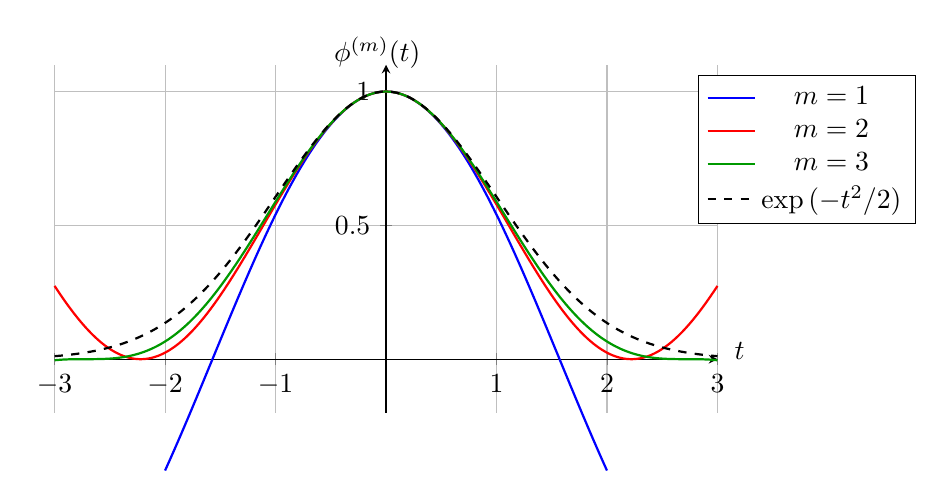
\begin{tikzpicture}
			\begin{axis}[
			width=10cm,
			height=6cm,
			xlabel={},
			ylabel={},
			legend style={at={(0.97,0.97)}, anchor=north west},
			domain=-3:3,
			ylabel style={
			yshift=10pt   % shift label up by 10pt
			},
			samples=400,
			ymin=-0.2, ymax=1.1,
			axis lines=middle,
			clip=false,
			grid=both,
			]
			\addplot[thick, blue,domain=-2:2] {cos(x/sqrt(1) r)^1};
			\addlegendentry{$m=1$}
			\addplot[thick, red] {cos(x/sqrt(2) r)^2};
			\addlegendentry{$m=2$}
			\addplot[thick, green!60!black] {cos(x/sqrt(3) r)^3};
			\addlegendentry{$m=3$}
			\addplot[thick, dashed, black] {exp(-x^2/2)};
			\addlegendentry{$\exp\,(-t^2/2)$}
			\node[anchor=south, rotate=0] at (axis cs:-0.08,1.05) {$\phi^{(m)}(t)$};
			\node[anchor=north, rotate=0] at (axis cs: 3.2,0.1) {$t$};
			\end{axis}
			\end{tikzpicture}
			\caption{\Glspl{characteristicfunc} of normalized sums of \gls{iid} \glspl{rv} $x^{(\sampleidx)} \in \{-1,1\}$ 
			for $\sampleidx=1,\ldots,\samplesize$ compared to the Gaussian limit.}
		\end{figure}
		See also: \gls{rv}, \gls{gaussrv}.},
	first={central limit theorem (CLT)},
	text={CLT}
}

\newglossaryentry{GaussProc}
{name={Gauß-Prozess (GP)},
	description={Ein \index{Gauß-Prozess (GP)}Gauß-Prozess ist eine Familie von \gls{rv}s 
		$\{f(\featurevec)\}_{\featurevec \in \featurespace}$, die durch Eingabewerte $\featurevec$ 
		aus einem Eingaberaum $\featurespace$ indiziert sind. Für jede endliche Teilmenge 
		$\featurevec^{(1)}, \ldots, \featurevec^{(\samplesize)} \in \featurespace$ 
		haben die entsprechenden \gls{rv}s $f(\featurevec^{(1)}), \ldots, f(\featurevec^{(\samplesize)})$ 
		eine gemeinsame multivariate Normalverteilung:
		\[
		\left( f(\featurevec^{(1)}), \ldots, f(\featurevec^{(\samplesize)}) \right) \sim \mathcal{N}(\boldsymbol{\mu}, \mathbf{K}).
		\]
		Für einen festen Eingaberaum $\featurespace$ ist ein Gauß-Prozess vollständig definiert durch:
		\begin{itemize}
			\item eine \gls{mean}-Funktion $\mu(\featurevec) = \expect\{ f(\featurevec)\}$,
			\item und eine Kovarianzfunktion $\kernelmap{\featurevec}{\featurevec'}= \expect\{ \big(f(\featurevec)-\mu(\featurevec)\big) \big(f(\featurevec')-\mu(\featurevec')\big) \big\}$.
		\end{itemize}
		\textbf{Beispiel.} Die Temperaturverteilung über Finnland zu einem bestimmten Zeitpunkt kann als \gls{realization} eines Gauß-Prozesses $f(\featurevec)$ interpretiert werden, wobei jeder Eingabewert $\featurevec = (\text{lat}, \text{lon})$ eine geografische Position darstellt. Temperaturmessungen von \gls{fmi}-Wetterstationen liefern Stichproben von $f(\featurevec)$ an bestimmten Orten (siehe Abb.\ \ref{fig_gp_FMI}). Ein Gauß-Prozess ermöglicht es, die Temperatur in der Nähe von \gls{fmi}-Wetterstationen vorherzusagen und die Unsicherheit dieser Vorhersagen zu quantifizieren.
		\begin{figure}[H]
			\begin{center}
				\begin{tikzpicture}
					\begin{axis}[
						axis equal,
						hide axis,
						scale=1.2,
						xmin=17, xmax=32,
						ymin=55, ymax=71,
						clip=true
						]
						% --- Finnland-Grenze (Polylinie) ---
						\addplot[
						color=black,
						thick
						] table [x=lon, y=lat, col sep=comma] {assets/finland_border.csv};
						% --- FMI-Messstationen ---
						\addplot[
						only marks,
						mark=*,
						mark options={fill=blue},
						color=black
						] table [x=lon, y=lat, col sep=comma] {assets/fmi_stations_subset.csv};
						% Manuelle Achsen zeichnen
						\draw[->, thick] (axis cs:19,59) -- (axis cs:25.5,59) node[anchor=west] {lon};
						\draw[->, thick] (axis cs:19,59) -- (axis cs:19,65.5) node[anchor=south] {lat};
					\end{axis}
				\end{tikzpicture}
				\vspace*{-15mm}
			\end{center}
			\caption{Die Temperaturverteilung über Finnland kann als \gls{realization} 
				eines Gauß-Prozesses interpretiert werden, der durch geografische Koordinaten indiziert ist und an \gls{fmi}-Wetterstationen (blaue Punkte) abgetastet wird. \label{fig_gp_FMI}}
	\end{figure}},
	first = {Gauß-Prozess},
	text = {GP}
}

	
\newglossaryentry{trustAI}
{name={Vertrauenswürdige Künstliche Intelligenz (trustworthy AI)},
	description={Neben den \gls{compasp}en und \gls{statasp}en gibt es einen dritten 
		Entwurfsaspekt für \gls{ml}-Methoden: Vertrauenswürdigkeit\index{trustworthy AI} 
		\cite{pfau2024engineeringtrustworthyaideveloper}. 
		Die EU hat sieben zentrale Anforderungen (Key Requirements, KRs) für 
		vertrauenswürdige \gls{ai} aufgestellt (die typischerweise auf \gls{ml}-Methoden basieren)
		\cite{ALTAIEU}:
		\begin{enumerate}[label=\arabic*)]
			\item KR1 – Vorrang menschlichen Handelns und menschliche Aufsicht,
			\item KR2 – Technische Robustheit und Sicherheit,
			\item KR3 – Datenschutz und Daten-Governance,
			\item KR4 – Transparenz,
			\item KR5 – Vielfalt, Nichtdiskriminierung und Fairness,
			\item KR6 – Gesellschaftliches und ökologisches Wohlergehen,
			\item KR7 – Rechenschaftspflicht.
		\end{enumerate}
	},
	first={Vertrauenswürdige Künstliche Intelligenz (trustworthy AI)},
	text={Vertrauenswürdige Künstliche Intelligenz}
}
	
\newglossaryentry{sqerrloss}
{name={quadratische Verlustfunktion},
	description={Die quadratische Verlustfunktion \index{quadratische Verlustfunktion} \gls{loss} 
		misst den \gls{prediction}fehler einer \gls{hypothesis} $\hypothesis$ 
		bei der Vorhersage eines numerischen \gls{label}s $\truelabel \in \mathbb{R}$ 
		anhand der \gls{feature}s $\featurevec$ eines \gls{datapoint}. Er ist definiert als
		\begin{equation} 
			\nonumber
			%	\label{equ_squared_loss_gls}
			\lossfunc{(\featurevec,\truelabel)}{\hypothesis} \defeq \big(\truelabel - \underbrace{\hypothesis(\featurevec)}_{=\predictedlabel} \big)^{2}. 
		\end{equation}
	},
	first={quadratische Verlustfunktion},
	text={quadratische Verlustfunktion}
}


\newglossaryentry{projection}
{name={Projektion}, 
	description={Betrachten wir einen Teilsatz $\paramspace \subseteq \mathbb{R}^{\dimlocalmodel}$ 
		des $\dimlocalmodel$-dimensionalen \gls{euclidspace}. Wir definieren die Projektion $\projection{\paramspace}{\weights}$
		eines Vektors $\weights \in \mathbb{R}^{\dimlocalmodel}$ auf $\paramspace$ als
		\begin{equation} 
			\label{equ_def_proj_generic_dict}
			\projection{\paramspace}{\weights} = \argmin_{\weights' \in \paramspace} \normgeneric{\weights - \weights'}{2}. 
		\end{equation}
		Mit anderen Worten: $\projection{\paramspace}{\weights}$ ist der Vektor in $\paramspace$, 
		der $\weights$ am nächsten liegt. Die Projektion ist nur für solche Teilmengen $\paramspace$ wohldefiniert, 
		für die das obige \gls{minimum} existiert \cite{BoydConvexBook}.},
	first={Projektion},
	text={Projektion}
}

\newglossaryentry{projgd}{
	name={projizierter Gradientenabstieg (projizierter GD)},
	description={
		Betrachten wir eine auf \gls{erm} basierende Methode, die ein parametriertes \gls{model} 
		mit einem \gls{paramspace} $\paramspace \subseteq \mathbb{R}^{\dimlocalmodel}$ verwendet. 
		Selbst wenn die \gls{objfunc} von \gls{erm} \gls{smooth} ist, können wir den einfachen 
		\gls{gd} nicht verwenden, da dieser keine Nebenbedingungen für die Optimierungsvariable 
		(also die \glspl{modelparam}) berücksichtigt. \\
		Der projizierte \index{projizierter Gradientenabstieg (projizierter GD)} \gls{gd} erweitert 
		den einfachen \gls{gd}, um solche Nebenbedingungen zu berücksichtigen. 
		Ein einzelner Schritt des projizierten \gls{gd} besteht darin, zunächst einen \gls{gradstep} 
		durchzuführen und anschließend das Ergebnis auf den \gls{paramspace} zurückzuprojezieren.
		\begin{figure}[H]
			\begin{center}
				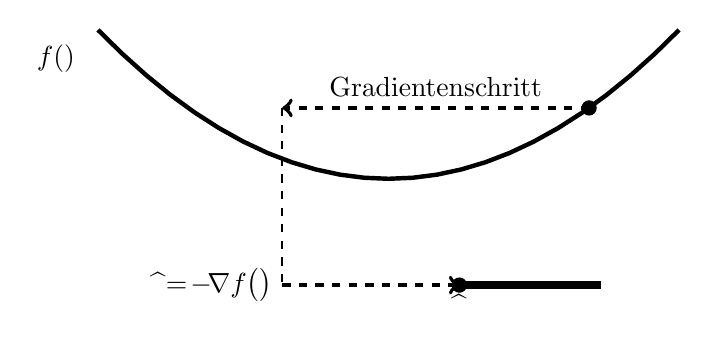
\begin{tikzpicture}[scale=0.9]
					\node [right] at (-5.1,1.7) {$f(\weights)$} ;
					\draw[ultra thick, domain=-4.1:4.1] plot (\x,  {(1/8)*\x*\x});
					\draw [fill] (2.83,1) circle [radius=0.1] node[right] {$\weights$};
					\draw[line width =0.5mm,dashed,->] (2.83,1) -- node[midway,above] {Gradientenschritt} (-1.5,1);
					\draw[line width =0.2mm,dashed] (-1.5,1) --(-1.5,-1.5)  node [below, left]{$\widehat{\weights}=\weights\!-\!\lrate \nabla f\big(\weights\big)$} ;
					\draw[line width =0.5mm,dashed,->] (-1.5,-1.5)  -- node[midway,above] {} (1,-1.5) ; 
					\draw [fill] (1,-1.5) circle [radius=0.1] node[below] {$\projection{\paramspace}{\widehat{\weights}}$};
					\draw[line width=1mm] (1,-1.5) -- (3,-1.5) node[midway, above] {$\paramspace$};
				\end{tikzpicture}
				\vspace*{-5mm}
			\end{center}
			\caption{Projizierter \gls{gd} erweitert einen einfachen \gls{gradstep} durch eine \gls{projection} zurück auf die zulässige Menge $\paramspace$.}
			\label{fig_projected_GD_dict}
		\end{figure}
	},
	first={projizierter Gradientenabstieg (projizierter GD)},
	text={projizierter GD}
}

\newglossaryentry{diffpriv}{
	name=differenzielle Privatsphäre (DP),
	description={
		Betrachten wir eine \gls{ml}-Methode $\algomap$, 
		die ein \gls{dataset} (z.\,B.\ das \gls{trainset} im Rahmen von \gls{erm}) einliest 
		und ein Ergebnis $\algomap(\dataset)$ liefert. Dieses Ergebnis kann entweder aus den 
		gelernten \glspl{modelparam} oder den \gls{prediction}s für bestimmte \gls{datapoint}s bestehen. \\
		Die differenzielle \index{differenzielle Privatsphäre (DP)} Privatsphäre (DP) ist ein präzises Maß 
		für die \gls{privleakage}, die durch die Offenlegung dieses Ergebnisses entsteht. 
		Grob gesagt ist eine \gls{ml}-Methode dann differentielle privat, wenn sich die 
		\gls{probdist} des Ausgabewerts $\algomap(\dataset)$ nicht wesentlich ändert, 
		wenn das \gls{sensattr} eines einzelnen \gls{datapoint} im \gls{trainset} verändert wird. \\
		Wichtig ist, dass DP auf einem \gls{probmodel} der \gls{ml}-Methode basiert – 
		das heißt, wir interpretieren $\algomap(\dataset)$ als \gls{realization} einer \gls{rv}. 
		Die notwendige Zufälligkeit im Ergebnis kann durch gezieltes Hinzufügen einer 
		Realisierung einer zusätzlichen \gls{rv} (also durch das Hinzufügen von Rauschen) 
		erzeugt werden.
	},
	first = {differenzielle Privatsphäre (DP)},
	text={DP}
}

\newglossaryentry{robustness}
{name={Robustheit},
	description={\textbf{Robustheit}\index{Robustheit} ist eine zentrale Anforderung für \gls{trustAI}. 
	Sie bezeichnet die Eigenschaft eines \gls{ml}-Systems, auch unter verschiedenen Arten von Störungen 
	eine akzeptable Leistung aufrechtzuerhalten. Solche Störungen können gezielte Veränderungen der 
	\glspl{feature} eines \gls{datapoint} sein, um die von einem trainierten \gls{ml}-\gls{model} gelieferten 
	\glspl{prediction} zu manipulieren.\\
	Zur Robustheit zählt auch die \gls{stability} von auf \gls{erm} basierenden Methoden gegenüber 
	Störungen im \gls{trainset}. Solche Störungen können beispielsweise im Rahmen von 
	\gls{datapoisoning}-\glspl{attack} auftreten.\\
	Siehe auch: \gls{trustAI}, \gls{ml}, \gls{feature}, \gls{datapoint}, \gls{prediction}, \gls{model}, 
	\gls{stability}, \gls{erm}, \gls{trainset}, \gls{datapoisoning}, \gls{attack}.}, 
	first={Robustheit}, 
	text={Robustheit}
}


\newglossaryentry{stability}{
	name={Stabilität},
	description={
		Die \index{Stabilität} \textbf{Stabilität} ist eine wünschenswerte Eigenschaft einer \gls{ml}-Methode $\algomap$, 
		die ein \gls{dataset} $\dataset$ (z.\,B.\ ein \gls{trainset}) auf eine Ausgabe $\algomap(\dataset)$ abbildet. 
		Die Ausgabe $\algomap(\dataset)$ kann entweder aus den gelernten \glspl{modelparam} oder aus 
		den \gls{prediction}s eines trainierten \gls{model} für einen bestimmten \gls{datapoint} bestehen. \\
		Intuitiv ist $\algomap$ stabil, wenn kleine Änderungen im Eingabe-\gls{dataset} $\dataset$ nur zu 
		kleinen Änderungen in der Ausgabe $\algomap(\dataset)$ führen. Es existieren mehrere formale 
		Begriffsbildungen von Stabilität, mit denen sich Schranken für den \gls{generalization}-Fehler oder das 
		\gls{risk} der Methode herleiten lassen (siehe \cite[Kap.~13]{ShalevMLBook}). \\
		Zur Veranschaulichung betrachte die drei in Abbildung~\ref{fig_three_data_stability} dargestellten \gls{dataset}s, 
		die unabhängig voneinander aus derselben \gls{data}-erzeugenden \gls{probdist} gezogen wurden. 
		Da die optimalen \glspl{modelparam} durch diese zugrunde liegende \gls{probdist} bestimmt sind, 
		sollte eine genaue \gls{ml}-Methode $\algomap$ für alle drei \gls{dataset}s dieselbe (oder eine sehr ähnliche) 
		Ausgabe $\algomap(\dataset)$ liefern. Mit anderen Worten: Eine sinnvolle $\algomap$ muss robust 
		gegenüber der Variabilität in \gls{sample}-\gls{realization}en aus derselben \gls{probdist} sein – 
		d.\,h.\ sie muss stabil sein.
		\begin{figure}[H]
			\centering
			\begin{tikzpicture}
				\begin{axis}[
					axis lines=none,
					xlabel={$\sampleidx$},
					legend pos=north west,
					ymin=0, ymax=10,
					xtick={1,2,3,4,5},
					grid style=dashed,
					every axis plot/.append style={very thick}
					]
					% Dataset 1
					\addplot+[only marks,mark=*] coordinates {
						(1,2) (2,4) (3,3) (4,5) (5,7)
					};
					% Dataset 2
					\addplot+[only marks,mark=square*] coordinates {
						(1,3) (2,2) (3,6) (4,4) (5,5)
					};
					% Dataset 3
					\addplot+[only marks,mark=triangle*] coordinates {
						(1,5) (2,7) (3,4) (4,6) (5,3)
					};
				\end{axis}
			\end{tikzpicture}
			\caption{Drei \gls{dataset}s $\dataset^{(*)}$, $\dataset^{(\square)}$ und $\dataset^{(\triangle)}$, 
				die jeweils unabhängig aus derselben \gls{data}-erzeugenden \gls{probdist} gezogen wurden. 
				Eine stabile \gls{ml}-Methode sollte bei Training auf einem dieser \gls{dataset}s jeweils 
				ähnliche Ausgaben liefern. \label{fig_three_data_stability}}
		\end{figure}
	},
	first = {Stabilität},
	text = {Stabilität}
}

\newglossaryentry{privprot}{
	name={Privatsphärenschutz},
	description={
		\index{Privatsphärenschutz} Betrachte eine \gls{ml}-Methode $\algomap$, die ein \gls{dataset} $\dataset$ 
		als Eingabe erhält und eine Ausgabe $\algomap(\dataset)$ liefert. Die Ausgabe kann die gelernten 
		\glspl{modelparam} $\widehat{\weights}$ oder die \gls{prediction} $\learnthypothesis(\featurevec)$ 
		für einen bestimmten \gls{datapoint} mit \gls{feature}n $\featurevec$ sein. \\
		Viele wichtige \gls{ml}-Anwendungen verarbeiten \gls{datapoint}s, die Menschen repräsentieren. 
		Jeder \gls{datapoint} ist charakterisiert durch \gls{feature}n $\featurevec$, eventuell ein \gls{label} $\truelabel$ 
		und ein \gls{sensattr} $\sensattr$ (z.\,B.\ eine kürzliche medizinische Diagnose). \\
		Grob gesagt bedeutet Privatsphärenschutz, dass es unmöglich sein sollte, aus der Ausgabe 
		$\algomap(\dataset)$ Rückschlüsse auf die \gls{sensattr}s einzelner \gls{datapoint}s in $\dataset$ zu ziehen. 
		Mathematisch verlangt Privatsphärenschutz, dass die Abbildung $\algomap(\dataset)$ nicht invertierbar ist. \\
		Im Allgemeinen reicht es jedoch nicht aus, $\algomap(\dataset)$ nur nicht invertierbar zu machen. 
		Vielmehr muss $\algomap(\dataset)$ hinreichend nicht invertierbar sein.
	},
	first = {Privatsphärenschutz},
	text = {Privatsphärenschutz}
}

\newglossaryentry{privleakage}{
	name={Privacy Leakage (Informationsleckage)},
	description={
		Betrachte eine \gls{ml}-Anwendung, die ein \gls{dataset} $\dataset$ verarbeitet und 
		eine Ausgabe liefert, z. B. \gls{prediction}en für neue \gls{datapoint}e. Privacy Leakage 
		entsteht, wenn die Ausgabe Informationen über eine private (oder sensible) \gls{feature} 
		eines \gls{datapoint}es (z. B. einer Person) aus $\dataset$ enthält. 
		Basierend auf einem \gls{probmodel} für die \gls{data}-Erzeugung kann man die Privacy Leakage 
		über die \gls{mutualinformation} zwischen der Ausgabe und dem sensiblen \gls{feature} messen. 
		Eine weitere quantitative Messgröße für Privacy Leakage ist die \gls{diffpriv}. 
		Die Zusammenhänge verschiedener Privacy-Maße wurden in der Literatur untersucht 
		(siehe \cite{InfThDiffPriv}).
	},
	first={Privacy Leakage (Informationsleckage)},
	text={Privacy Leakage}
}

\newglossaryentry{probmodel}
{
	name=probabilistisches Modell,
	description={Ein probabilistisches \gls{model}\index{probabilistisches Modell} interpretiert \gls{datapoint}s 
		als \gls{realization}s von \gls{rv}s mit einer gemeinsamen \gls{probdist}. Diese gemeinsame \gls{probdist} 
		umfasst typischerweise \gls{parameters}, die entweder manuell festgelegt oder durch statistische 
		Schätzverfahren wie die \gls{maxlikelihood}-Schätzung \cite{LC} erlernt werden.}, 
	first = {probabilistisches Modell}, text={probabilistisches Modell} , plural={probabilistische Modelle}
}

\newglossaryentry{mean}
{
	name=Erwartungswert,
	description={Der \index{Erwartungswert} Erwartungswert einer \gls{rv} $\featurevec$, 
		die Werte in einem \gls{euclidspace} $\mathbb{R}^{\dimlocalmodel}$ annimmt, ist der 
		\gls{expectation} $\expect\{\featurevec\}$. Er ist als Lebesgue-Integral von 
		$\featurevec$ bezüglich der zugrunde liegenden \gls{probdist} $P$ definiert (siehe z.\,B. \cite{BillingsleyProbMeasure} oder \cite{RudinBookPrinciplesMatheAnalysis}), also:
		\[
		\expect\{\featurevec\} = \int_{\mathbb{R}^{\dimlocalmodel}} \vx \, \mathrm{d}P(\vx).
		\]
		Der Begriff wird auch für den Durchschnitt einer endlichen Folge 
		$\vx^{(1)}, \ldots, \vx^{(\samplesize)} \in \mathbb{R}^{\dimlocalmodel}$ verwendet. 
		Diese beiden Definitionen sind im Wesentlichen äquivalent. Tatsächlich lässt sich 
		die Folge $\vx^{(1)}, \ldots, \vx^{(\samplesize)}$ verwenden, um eine diskrete 
		\gls{rv} $\widetilde{\vx} = \vx^{(I)}$ zu konstruieren, wobei der Index $I$ 
		gleichverteilt aus der Menge $\{1, \ldots, \samplesize\}$ gewählt wird. 
		Der Erwartungswert von $\widetilde{\vx}$ ist dann genau der Durchschnitt 
		$\frac{1}{\samplesize} \sum_{\sampleidx=1}^{\samplesize} \vx^{(\sampleidx)}$.},
	first = {Erwartungswert}, text={Erwartungswert} 
}
%hier hängt der Name vom Kontext ab, es sieht so aus als würde "Erwartungswert" vor allem für Wahrscheinlichkeiten und Mittelwert eher grob im mathematischen bereich genutzt. Ich habe auch "Statistisches Mittel", Arithmetsisches mittel gefunden, das muss nochmal angeschaut werden.

\newglossaryentry{median}
{name={Median}, 
plural={Mediane},
description={Ein\index{Median} Median $\med\,(x)$ einer reellwertigen \gls{rv} $x$ 
 		ist jede Zahl $M \in \mathbb{R}$, sodass $\prob{ x \leq M} \geq 1/2$ und 
		$\prob{ x \geq M} \geq 1/2$ 
		(siehe Abb. \ref{fig_median1_dict}) \cite{LC}. 
 		\begin{figure}[H]
			\begin{center}
			\begin{tikzpicture}
 			\begin{axis}[
    			axis lines=middle,
    			xlabel={},
    			ylabel={},
    			ymin=0, ymax=1.1,
    			xmin=-2, xmax=6,
    			xtick=\empty,
    			ytick={0,1/2,1},
    			domain=-2:6,
    			samples=200,
    			width=10cm,
    			height=6cm,
    			smooth,
    			enlargelimits=true,
    			clip=false
  			]
    			% Verschobene Sigmoid-KDF
			\addplot[thick, blue, name path=cdf] {1/(1 + exp(-(x - 1)))} node[pos=0.5, above, yshift=15pt] {$\prob{x \leq \eta}$};    
    			\draw[dashed, gray] (axis cs:1,0) -- (axis cs:1,0.5); % vertikal
    			\draw[dashed, gray] (axis cs:-2,0.5) -- (axis cs:1,0.5); % horizontal
    			% Medianpunkt markieren
   			\filldraw[red] (axis cs:1,0.5) circle (2pt);
  		    \node[below] at (axis cs:1,0) {$M$};
			\node[above right] at (axis cs:6.3,0) {$\eta$};
  			\end{axis}
			\end{tikzpicture} 
			\end{center}
			\caption{Der Median einer reellwertigen \gls{rv} ist jede Zahl $M$, 
			die $\mathbb{R}$ in zwei Teilmengen mit gleicher \gls{probability} teilt. \label{fig_median1_dict}}
 		\end{figure}  
 		Der Median $\med\,(\dataset)$ 
 		eines \gls{dataset} $\dataset = \{ x^{(1)}, \ldots, x^{(\samplesize)} \in \mathbb{R} \}$ 
 		kann über eine spezifische \gls{rv} $\tilde{x}^{(\dataset)}$ definiert werden, die natürlich mit $\dataset$ assoziiert ist. 
 		Insbesondere ist diese \gls{rv} auf dem \gls{samplespace} $\{1, \ldots, \samplesize\}$ definiert durch $\tilde{x}^{(\dataset)} \defeq x^{(I)}$, wobei der Index $I$ gleichverteilt zufällig gewählt wird, d.h., $\prob{I = \sampleidx}=1/\samplesize$ für alle $\sampleidx=1, \ldots, \samplesize$. Wenn die \gls{rv} $x$ integrierbar ist, löst jeder Median von $x$ das \gls{optproblem}: 
 		$$\min_{x' \in \mathbb{R}} \expect{|x - x'|}.$$ 
		Für die obige \gls{rv} $\tilde{x}$ (aus einem \gls{dataset} $\dataset$ konstruiert) entspricht dieses \gls{optproblem} \gls{erm} auf $\dataset$ unter Verwendung von \gls{abserr}. 
 		Ähnlich wie der \gls{mean} kann der Median eines \gls{dataset} $\dataset$ auch zur Schätzung von \glspl{parameter} eines zugrunde liegenden \gls{probmodel} verwendet werden. Im Vergleich zum \gls{mean} ist der Median robuster gegenüber \glspl{outlier}. Zum Beispiel ändert sich der Median eines \gls{dataset} $\dataset$ mit mehr als einem \gls{datapoint} nicht, selbst wenn wir das größte Element von $\dataset$ beliebig vergrößern (siehe Abb. \ref{fig_median2_dict}). Im Gegensatz dazu würde der \gls{mean} beliebig ansteigen.
		\begin{figure}[H]
		\centering
		\begin{tikzpicture}[scale=0.7, y=0.5cm, x=0.5cm]
			\begin{scope}
				\foreach \x/\y in {
					1/2, 4/3, 7/4
				} {
					\draw[dashed, gray] (\x, 0) -- (\x, \y);
					\filldraw[blue] (\x, \y) circle (2pt);
					\node[circle, inner sep=0pt] (ptA\x) at (\x, \y) {};
				}
				\draw[dashed, thick] (0.5, 3) -- (10.5, 3) node[right] {$\med\,(\dataset)\!=\!{\rm mean}(\dataset)$};
				\node at (7.5, -4) {(a)};
			\end{scope}
			\begin{scope}[xshift=12cm]
				\foreach \x/\y in {
					1/2, 4/3, 7/10
				} {
					\draw[dashed, gray] (\x, 0) -- (\x, \y);
					\filldraw[blue] (\x, \y) circle (2pt);
					\node[circle, inner sep=0pt] (ptB\x) at (\x, \y) {};
				}
				\draw[dashed, thick] (0.5, 7.5) -- (10.5, 7.5) node[right] 
				{${\rm mean}\,\big(\widetilde{\dataset}\big)$};
				\draw[dashed, thick] (0.5, 3) -- (10.5, 3) node[right] 
				{$\med\,\big(\widetilde{\dataset}\big)$};
				\node[above right=2pt and 2pt, red] at (ptB7) {\gls{outlier}};
				\node at (7.5, -4) {(b)};
			\end{scope}
		\end{tikzpicture}
		\caption{Der Median ist robust gegenüber \gls{outlier}-Kontamination. (a) Originales \gls{dataset} $\dataset$. (b) Rauschbehaftetes \gls{dataset} $\widetilde{\dataset}$ mit einem \gls{outlier}. \label{fig_median2_dict}}
		\end{figure}
		Siehe auch: \gls{mean}, \gls{outlier}, \gls{robustness}, \gls{ladregression}.}, 
first={Median}, 
type=math,
text={Median} 
}


\newglossaryentry{variance}
{
	name={Varianz},
	name=Varianz,
	description={Die \index{Varianz} Varianz einer reellwertigen \gls{rv} $\feature$ ist definiert als der 
		\gls{expectation} $\expect\big\{ \big( x - \expect\{x \} \big)^{2} \big\}$ des quadrierten Abstands zwischen 
		$\feature$ und ihrem \gls{expectation} $\expect\{x \}$. Diese Definition lässt sich auf vektorwertige 
		\gls{rv}s $\featurevec$ erweitern als 
		\[
		\expect\big\{ \big\| \featurevec - \expect\{\featurevec \} \big\|_{2}^{2} \big\}.
		\]
	}, 
	first={Varianz}, text={Varianz} 
}

\newglossaryentry{nn}
{
	name={nächster Nachbar (NN)},
	description={NN\index{nächster Nachbar (NN)}-Methoden lernen eine \gls{hypothesis} 
		$\hypothesis: \featurespace \rightarrow \labelspace$, deren Funktionswert $\hypothesis(\featurevec)$ 
		allein durch die nächstgelegenen \gls{neighbors} in einem gegebenen \gls{dataset} bestimmt wird. 
		Verschiedene Methoden verwenden unterschiedliche Metriken zur Bestimmung der nächsten 
		\gls{neighbors}. Wenn \gls{datapoint}s durch numerische \gls{featurevec}s beschrieben sind, 
		kann beispielsweise der euklidische Abstand als Metrik verwendet werden.},
	first={nächster Nachbar (NN)}, text={NN}
}

\newglossaryentry{neighborhood}
{
	name={Nachbarschaft},
	description={Die \index{Nachbarschaft} Nachbarschaft eines Knotens $\nodeidx \in \nodes$ 
		ist die Teilmenge der Knoten, die die \gls{neighbors} von $\nodeidx$ bilden.},
	first={Nachbarschaft}, text={Nachbarschaft}, plural={Nachbarschaften}
}

\newglossaryentry{neighbor}
{name={Nachbar},
description={Ein\index{Nachbar} Nachbar eines Knotens $\nodeidx \in \nodes$ 
	innerhalb eines ungerichteten \gls{graph} ist ein Knoten $\nodeidx' \in \nodes \setminus \{ \nodeidx\}$, 
	der über eine Kante mit dem Knoten $\nodeidx$ verbunden ist.
			\\ 
	See also: \gls{graph}.},
first={Nachbar},
firstplural={Nachbarn}, 
plural={Nachbarn}, 
text={Nachbar} 
}


\newglossaryentry{bias}
{
	name={Bias},
	description={Betrachten wir eine \index{Bias} \gls{ml}-Methode mit einem parametrisierbaren \gls{hypospace} $\hypospace$. 
		Diese Methode lernt die \glspl{modelparam} $\weights \in \mathbb{R}^{\dimlocalmodel}$ anhand des \gls{dataset}
		\[
		\dataset = \big\{ \pair{\featurevec^{(\sampleidx)}}{\truelabel^{(\sampleidx)}} \big\}_{\sampleidx=1}^{\samplesize}.
		\]
		Zur Analyse der Eigenschaften dieser \gls{ml}-Methode interpretieren wir die \gls{datapoint}s typischerweise 
		als \gls{realization}s von \gls{iid} \gls{rv}s:
		\[
		\truelabel^{(\sampleidx)} = \hypothesis^{(\overline{\weights})}\big( \featurevec^{(\sampleidx)} \big) + \bm{\varepsilon}^{(\sampleidx)}, 
		\quad \sampleidx=1,\ldots,\samplesize.
		\]
		Die \gls{ml}-Methode lässt sich dann als Schätzer $\widehat{\weights}$ interpretieren, der aus dem Datensatz $\dataset$ 
		(z.\,B. durch Lösung des \gls{erm}) berechnet wird. Der (quadratische) Bias dieses Schätzers $\widehat{\weights}$ ist definiert als:
		\[
		\biasterm^{2} \defeq \big\| \expect \{ \widehat{\weights} \} - \overline{\weights} \big\|_{2}^{2}.
		\]},
	first={Bias}, text={Bias}
}


\newglossaryentry{classification}
{
	name={Klassifikation},
	description={Die \index{Klassifikation} Klassifikation ist die Aufgabe, einem gegebenen 
		\gls{datapoint} basierend auf dessen Merkmalen $\featurevec$ ein diskretwertiges Label $\truelabel$ 
		zuzuordnen. Das Label $\truelabel$ gehört zu einer endlichen Menge, etwa 
		$\truelabel \in \{-1,1\}$ oder $\truelabel \in \{1,\ldots,19\}$, und repräsentiert die Kategorie, 
		zu der der jeweilige \gls{datapoint} gehört.},
	first={Klassifikation}, text={Klassifikation}

}

\newglossaryentry{privfunnel}
{
	name={Privacy Funnel},
	description={Der \index{Privacy Funnel} Privacy Funnel ist eine Methode zur Erlernung 
		privatsphärefreundlicher \gls{feature}s von \gls{datapoint}s \cite{PrivacyFunnel}.},
	first={Privacy Funnel}, text={Privacy Funnel}
}

\newglossaryentry{condnr}
{
	name={Konditionszahl},
	description={Die \index{Konditionszahl} Konditionszahl $\kappa(\mathbf{Q}) \geq 1$ einer positiv definiten 
		Matrix $\mathbf{Q} \in \mathbb{R}^{\featurelen \times \featurelen}$ ist definiert als das Verhältnis 
		$\alpha / \beta$ der größten $\alpha$ zur kleinsten $\beta$ \gls{eigenvalue} von $\mathbf{Q}$. 
		Die Konditionszahl ist ein wichtiges Hilfsmittel zur Analyse von \gls{ml}-Methoden. 
		Die Rechenkomplexität von \gls{gdmethods} bei \gls{linreg} hängt wesentlich von der 
		Konditionszahl der Matrix $\mQ = \mX \mX^{T}$ ab, wobei $\mX$ die \gls{featuremtx} 
		des \gls{trainset} ist. Aus rechentechnischer Sicht bevorzugt man daher \gls{feature}s 
		von \gls{datapoint}s, bei denen $\mQ$ eine Konditionszahl nahe $1$ besitzt.},
	first={Konditionszahl}, text={Konditionszahl}
}

\newglossaryentry{classifier}
{name={Klassifikator},
description={Ein Klassifikator\index{Klassifikator} ist eine \gls{hypothesis} (d.h. eine \gls{map}) $\hypothesis(\featurevec)$, 
		die zur Vorhersage eines \gls{label} verwendet wird, das Werte aus einem endlichen \gls{labelspace} annimmt. 
		Wir könnten den Wert der \gls{function} $\hypothesis(\featurevec)$ selbst als \gls{prediction} $\predictedlabel$ für 
		das \gls{label} verwenden. Üblicherweise benutzt man jedoch eine \gls{map} $\hypothesis(\cdot)$, die eine 
		numerische Größe liefert. Die \gls{prediction} wird dann über einen einfachen Schwellenwertschritt erhalten. 
		Für ein binäres \gls{classification}-Problem mit einem \gls{labelspace} $\labelspace = \{-1,1\}$ 
		könnte man z.B. eine reellwertige \gls{hypothesis}-\gls{map} $\hypothesis(\featurevec) \in \mathbb{R}$ als Klassifikator verwenden. 
		Eine \gls{prediction} $\predictedlabel$ kann dann durch Thresholding bestimmt werden:
		 \begin{equation} 
		 	\label{equ_def_threshold_bin_classifier_dict}
		 	\predictedlabel =1   \mbox{ für } \hypothesis(\featurevec)\!\geq\!0 \mbox{ und } 	\predictedlabel =-1  \mbox{ sonst.}
	 		\end{equation}
		Ein Klassifikator kann über seine \glspl{decisionregion} $\decreg{a}$ charakterisiert werden, 
		für jeden möglichen \gls{label}-Wert $a \in \labelspace$.
					\\ 
		Siehe auch: \gls{hypothesis}, \gls{classification}, \gls{decisionregion}. },
first={Klassifikator},
text={Klassifikator} 
}


\newglossaryentry{emprisk}
{
	name={empirisches Risiko},
	description={Das empirische \gls{risk}\index{empirisches Risiko} 
		$\emprisk{\hypothesis}{\dataset}$ einer \gls{hypothesis} auf einem 
		\gls{dataset} $\dataset$ ist der durchschnittliche \gls{loss}, 
		den $\hypothesis$ beim Anwenden auf die \gls{datapoint}s in $\dataset$ verursacht.},
	first={empirisches Risiko}, text={empirisches Risiko}
}

\newglossaryentry{nodedegree}
{
	name={Knoten­grad},
	description={Der Grad\index{Knotengrad} $\nodedegree{\nodeidx}$ eines Knotens 
		$\nodeidx \in \nodes$ in einem ungerichteten \gls{graph} ist die Anzahl seiner 
		\gls{neighbors}, also 
		\[
		\nodedegree{\nodeidx} \defeq \big| \neighbourhood{\nodeidx} \big|.
		\]},
	first={Knotengrad}, text={Knotengrad}
}

\newglossaryentry{token}
{name={Token},
description={Ein \textit{Token} ist eine grundlegende Informationseinheit, 
	die durch Aufteilen einer Symbolfolge, wie z.B. eines Textstrings, 
	in kleinere Teile gewonnen wird. In der \gls{nlp} entsprechen Tokens 
	häufig Wörtern, Subwörtern oder Zeichen, die die \glspl{feature} 
	eines \gls{datapoint} bilden. Die Tokenisierung wandelt Rohtext 
	(z.B. ``Die Katze schläft'') in eine Sequenz von Tokens um 
	(z.B. [``Die'', ``Katze'', ``schläft'']), die anschließend in numerische 
	\glspl{featurevec} überführt werden können.}, 
first={Token}, 
firstplural={Tokens}, 
plural={Tokens}, 
text={Token}
}

\newglossaryentry{nlp}
{name={Natural Language Processing (NLP)},
description={NLP \index{Natural Language Processing (NLP)} 
	untersucht \gls{ml}-Methoden zur Analyse und Generierung menschlicher Sprache. 
	Typische NLP-Aufgaben umfassen Text-\gls{classification}, maschinelle Übersetzung, 
	Sentiment-Analyse und Fragebeantwortung. Moderne NLP-Systeme repräsentieren 
	Sprache als Sequenzen von \glspl{token} und trainieren \glspl{model}, die 
	kontextuelle Abhängigkeiten erfassen, z.B. mittels \glspl{attention}-basierter Methoden.\\
	Siehe auch: \gls{attention}, \gls{token}.}, 
first={Natural Language Processing (NLP)}, 
text={NLP}
}

\newglossaryentry{directedcyble}
{name={gerichteter Zyklus},
description={Ein gerichteter Zyklus\index{gerichteter Zyklus} in einem \gls{directedgraph} 
	$\graph=\pair{\nodes}{\edges}$ ist eine Sequenz von verschiedenen Knoten 
	$(\nodeidx_1, \nodeidx_2, \ldots, \nodeidx_k)$, so dass 
	$(\nodeidx_1, \nodeidx_2), (\nodeidx_2, \nodeidx_3), \ldots, (\nodeidx_{k-1}, \nodeidx_k), 
     (\nodeidx_k, \nodeidx_1) \in \edges$ gilt. In einem gerichteten Zyklus führt das Folgen 
	der Richtung jeder Kante schließlich zurück zum Startknoten, wodurch eine geschlossene Schleife entsteht.
	\begin{figure}[H]
	\centering
	\begin{tikzpicture}[>=Latex, node distance=1.4cm, thick]
	% Knoten
	  \coordinate (a1) at (90:1.5);
  	  \coordinate (a2) at (210:1.5);
      \coordinate (a3) at (330:1.5);
  % Gefüllte Kreise für Knoten
  	 \fill (a1) circle (2pt) node[above=3pt] {$\nodeidx_1$};
  	 \fill (a2) circle (2pt) node[below left=3pt] {$\nodeidx_2$};
  	 \fill (a3) circle (2pt) node[below right=3pt] {$\nodeidx_3$};
	% Gerichtete Kanten
	\draw[->] (a1) -- (a2);
	\draw[->] (a2) -- (a3);
	\draw[->] (a3) -- (a1);
	\end{tikzpicture}
	\caption{Ein gerichteter Zyklus, bestehend aus drei Knoten, die eine geschlossene Schleife bilden.}
	\end{figure}
	Das Vorhandensein eines gerichteten Zyklus verhindert, dass ein \gls{directedgraph} ein \gls{dag} ist.
					\\
	Siehe auch: \gls{directedgraph}, \gls{dag}.},
first={gerichteter Zyklus},
firstplural={gerichtete Zyklen}, 
plural={gerichtete Zyklen}, 
type=math, 
text={gerichteter Zyklus} 
}

\newglossaryentry{dag}
{name={gerichteter azyklischer Graph (DAG)},
description={Ein \index{gerichteter azyklischer Graph (DAG)}DAG ist ein \gls{directedgraph}, 
    der keine gerichteten Zyklen enthält. Formal gilt für einen DAG 
    $\graph = (\nodes, \edges)$, dass für jede Sequenz verschiedener Knoten 
    $(\nodeidx_1, \ldots, \nodeidx_k)$ die Existenz gerichteter Kanten 
    $(\nodeidx_1,\nodeidx_2), (\nodeidx_2,\nodeidx_3), \ldots, (\nodeidx_{k-1},\nodeidx_k)$ 
    impliziert, dass $(\nodeidx_k, \nodeidx_1) \notin \edges$ gilt.
	\begin{figure}[H]
		\centering
		\begin{tikzpicture}[>=Latex, node distance=1.4cm, thick, every node/.style={circle, fill=black, inner sep=1.5pt}]
		% --- Links: DAG (gerichtete Kette) ---
		\node (a1) {};
		\node[right=of a1] (a2) {};
		\node[right=of a2] (a3) {};
		\draw[->] (a1) -- (a2);
		\draw[->] (a2) -- (a3);
		% --- Rechts: gleicher Graph mit Zyklus ---
		\node[right=3.5cm of a3] (b1) {};
		\node[right=of b1] (b2) {};
		\node[right=of b2] (b3) {};
		\draw[->] (b1) -- (b2);
		\draw[->] (b2) -- (b3);
		\draw[->, bend left=40] (b3) to (b1); % hinzugefügte Kante erzeugt Zyklus
		\end{tikzpicture}
	\caption{Links: Ein DAG auf drei Knoten $\nodes=\{1,2,3\}$. Rechts: Ein weiterer 
	\gls{directedgraph} auf denselben Knoten, der kein DAG ist, da er einen 
	gerichteten Zyklus enthält.}
	\end{figure}
	Das Fehlen gerichteter Zyklen ermöglicht eine topologische Sortierung der Knoten, 
	sodass alle Kanten von früheren zu späteren Knoten in dieser Reihenfolge verlaufen. 
	Mehrere \gls{ml} \glspl{model}, wie z.B. \glspl{ann} oder \glspl{decisiontree}, 
	lassen sich natürlich als DAGs darstellen.\\
	Siehe auch: \gls{ann}, \gls{decisiontree}, \gls{directedgraph}.},
first={gerichteter azyklischer Graph (DAG)},
firstplural={gerichtete azyklische Graphen (DAGs)},
plural={DAGs},
type=math,
text={DAG}
}

\newglossaryentry{directedgraph}
{name={gerichteter Graph},
description={Ein gerichteter \gls{graph}\index{gerichteter Graph} enthält Kanten, 
	die eine Orientierung (oder Richtung) besitzen. Mathematisch besteht ein gerichteter 
	\gls{graph} $\graph=\pair{\nodes}{\edges}$ aus Knoten $\nodes$ und einer Menge 
	$\edges \subseteq \nodes \times \nodes$ gerichteter Kanten.
	\begin{figure}[H]
		\centering
		\begin{tikzpicture}[>=stealth, node distance=1.8cm]
  			\node[circle, draw, fill=black, inner sep=1.5pt, label=below:{$\nodeidx$}] (i) {};
  			\node[circle, draw, fill=black, inner sep=1.5pt, label=below:{$\nodeidx'$}] (ip) [right=of i] {};
  			\draw[->, >=Latex, line width=1pt, scale=1.3] (i) -- (ip);
		\end{tikzpicture}
	\caption{Die Kanten eines gerichteten \gls{graph} besitzen eine Orientierung (Richtung), die durch Pfeilspitzen angezeigt wird.}
	\end{figure}
	Wir können eine gerichtete Kante von einem Knoten $\nodeidx \in \nodes$ zu einem Knoten 
	$\nodeidx' \in \nodes$ durch das geordnete Paar $\pair{\nodeidx}{\nodeidx'}$ darstellen. 
	Gerichtete \glspl{graph} werden häufig zur Modellierung vernetzter Systeme oder 
	Netzwerke verwendet, z.B. Transportsysteme, elektronische Schaltungen oder biologische Prozesse \cite{NewmannBook}.\\
	Siehe auch: \gls{graph}.},
first={gerichteter Graph},
firstplural={gerichtete Graphen},
plural={gerichtete Graphen},
type=math,
text={gerichteter Graph}
}

\newglossaryentry{undirectedgraph}
{name={ungerichteter Graph},
description={Siehe \gls{graph}. 
\\
Siehe auch: \gls{graph}.},
first={ungerichteter Graph},
firstplural={ungerichtete Graphen},
plural={ungerichtete Graphen},
type=math,
text={ungerichteter Graph}
}

\newglossaryentry{simplefunction}
{name={einfache Funktion},
  description={Eine\index{einfache Funktion} einfache \gls{function} 
 		$f: \mathbb{R}^{\nrfeatures} \rightarrow \mathbb{R}$ ist eine \gls{measurable} 
 		\gls{function}, die nur endlich viele Werte annimmt. Anders gesagt,
 		$$f(\featurevec) = \sum_{\clusteridx=1}^{\nrcluster} \alpha_{\clusteridx} \mathcal{I}^{(\cluster^{(\clusteridx)})}(\featurevec),$$
 		mit der Indikator-\gls{function} $\mathcal{I}^{(\cluster)}$ einer 
 		Teilmenge $\cluster \subset \mathbb{R}^{\nrfeatures}$ und beliebigen 
 		Koeffizienten $\alpha_{1},\ldots,\alpha_{\nrcluster} \in \mathbb{R}$. 
 		Die Teilmengen $\cluster^{(1)},\ldots,\cluster^{(\nrcluster)}$ in der obigen 
 		Darstellung müssen \gls{measurable} sein und eine Partition von 
 		$\mathbb{R}^{\nrfeatures}$ bilden.\\
 		Siehe auch: \gls{LebesgueIntegral}, \gls{measurable}.}, 
 first={einfache Funktion}, 
 plural={einfache Funktionen}, 
 text={einfache Funktion}, 
 type=math
}

\newglossaryentry{LebesgueIntegral}
{name={Lebesgue-Integral},
	description={Das Lebesgue-Integral\index{Lebesgue-Integral} ordnet jeder integrierbaren \gls{function} 
	$f: \mathbb{R}^{\nrfeatures} \rightarrow \mathbb{R}$ eine Zahl 
	$\int_{\featurevec} f(\featurevec) d\featurevec$ zu, die als das Integral von $f$ bezeichnet wird. 
	Das Integral von $f$ kann als das Volumen interpretiert werden, das die \gls{function} 
	$f$ im Raum $\mathbb{R}^{\nrfeatures+1}$ einschließt. Es kann durch zunehmend genaue 
	Näherungen mittels \glspl{simplefunction} berechnet werden \cite[Ch. 1]{RudinBook}. 
	\begin{figure}[H]
		\centering
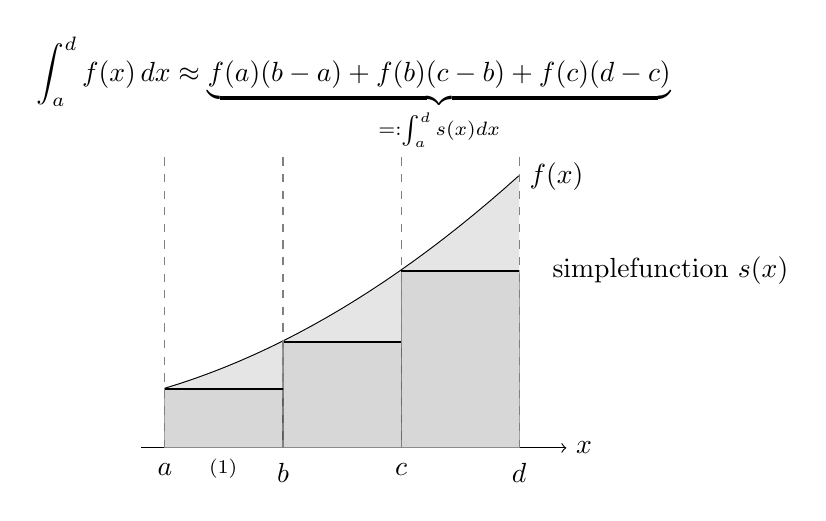
\begin{tikzpicture}[scale=1.5]
  % Achsen
  \draw[->] (-0.2,0) -- (3.4,0) node[right] {$x$};
  % Kontinuierliche Funktion f(x)
  \draw[thick,domain=0:3,smooth] plot(\x,{0.5+0.3*\x+0.1*\x*\x}) node[right] {$f(x)$};
  % Fläche unter f(x) schattieren
  \fill[gray!20] (0,0) -- plot[domain=0:3] (\x,{0.5+0.3*\x+0.1*\x*\x}) -- (3,0) -- cycle;
  % Treppenfunktion: linke Endpunkte der Intervalle [0,1], [1,2], [2,3]
  \draw[fill=gray!50,opacity=0.35] (0,0) rectangle (1,0.5);
  \node at (0.5,-0.2) {$\cluster^{(1)}$}; 
  \draw[fill=gray!50,opacity=0.35] (1,0) rectangle (2,0.9);
  \draw[fill=gray!50,opacity=0.35] (2,0) rectangle (3,1.5);
  % Linien der Treppenfunktion
  \draw[thick] (0,0.5)--(1,0.5);
  \draw[thick] (1,0.9)--(2,0.9);
  \draw[thick] (2,1.5)--(3,1.5);
  % Gepunktete Linien der Partition
  \foreach \x in {0,1,2,3} \draw[dashed,gray] (\x,0) -- (\x,2.5);
  % Beschriftungen
  \node[anchor=north] at (0,-0.05) {$a$};
  \node[anchor=north] at (1,-0.05) {$b$};
  \node[anchor=north] at (2,-0.05) {$c$};
  \node[anchor=north] at (3,-0.05) {$d$};
  \node at (1.6,3.0) {$\displaystyle \int_a^d f(x)\,dx \approx \underbrace{f(a)(b-a) + f(b)(c-b)+f(c)(d-c)}_{=:\int_a^d s(x)dx}$};
  \node [anchor=west] at (3.2,1.5) {\gls{simplefunction} $s(x)$};
\end{tikzpicture}
\end{figure}
Es ist nützlich, das Lebesgue-Integral als \gls{function} zu betrachten, die jede integrierbare 
\gls{function} $f$ auf den Wert ihres Integrals abbildet:
$$ f \mapsto \int_{\featurevec} f(\featurevec) d\featurevec.$$ 
Die präzise Definition dieser \gls{function}, einschließlich ihres \gls{domain}, 
welches die integrierbaren \glspl{function} umfasst, ist ein Grundpfeiler der 
Maßtheorie \cite[Ch. 1]{RudinBook}.
					\\ 
		Siehe auch: \gls{function}.},
	first={Lebesgue-Integral},
	type=math, 
	firstplural={Lebesgue-Integrale}
}

\newglossaryentry{cdf}
{name={kumulative Verteilungsfunktion (cdf)},
	description={Die \index{kumulative Verteilungsfunktion (cdf)} cdf 
	$\cdf{\feature}{\eta}$ einer reellen \gls{rv} $\feature$ ist definiert als \cite{AshProbMeasure,papoulis}
	$$\cdf{\feature}{\eta} \defeq \prob{\feature \leq \eta}.$$
					\\ 
		Siehe auch: \gls{pdf}, \gls{probdist}, \gls{rv}.},
	first={kumulative Verteilungsfunktion (cdf)},
	firstplural={kumulative Verteilungsfunktionen (cdfs)}, 
	plural={cdfs}, 
	type=math,
	text={cdf} 
}

\newglossaryentry{weightedgraph}
{name={gewichteter Graph},
	description={Ein \gls{graph}\index{gewichteter Graph}, dessen Kanten numerische Gewichte 
	erhalten. Typischerweise sind diese Kantengewichte nichtnegative reelle Zahlen. 
	Beispielsweise kann in einem Graphen, der ein Straßennetz darstellt, wobei die Knoten Kreuzungen 
	sind und die Kanten Straßenabschnitte darstellen, das Kantengewicht die Kapazität 
	(maximale Fahrzeuge pro Stunde) des Straßenabschnitts darstellen \cite{NewmannBook}.  
					\\ 
		Siehe auch: \gls{graph}.},
	first={gewichteter Graph},
	type=math,
	firstplural={gewichtete Graphen}, 
	plural={gewichtete Graphen}, 
	text={gewichteter Graph} 
}


\newglossaryentry{graph}
{
	name={Graph},
	description={Ein \index{Graph} Graph $\graph = \pair{\nodes}{\edges}$ ist ein Paar, bestehend aus 
		einer Knotenmenge $\nodes$ und einer Kantenmenge $\edges$. In der allgemeinsten Form wird ein Graph durch eine Abbildung beschrieben, 
		die jeder Kante $\edgeidx \in \edges$ ein Paar von Knoten zuordnet \cite{RockNetworks}. 
		Eine wichtige Familie von Graphen sind einfache ungerichtete Graphen. Ein einfacher ungerichteter Graph entsteht durch Identifikation 
		jeder Kante $\edgeidx \in \edges$ mit zwei verschiedenen Knoten $\{\nodeidx, \nodeidx'\}$. 
		Gewichtete Graphen spezifizieren zusätzlich numerische \gls{weights} $\edgeweight_{\edgeidx}$ für jede Kante $\edgeidx \in \edges$.},
	first={Graph}, text={Graph}, plural={Graphen}
}


\newglossaryentry{uncertainty}
{
	name={Unsicherheit},
	description={Unsicherheit\index{Unsicherheit} bezeichnet den Grad des Vertrauens — oder das Fehlen desselben — 
		in eine Größe wie eine \gls{model} \gls{prediction}, eine Parameterschätzung oder eine beobachtete \gls{datapoint}. 
		Im \gls{ml} entsteht Unsicherheit aus verschiedenen Quellen, darunter verrauschte \gls{data}, begrenzte Trainingsstichproben 
		oder Mehrdeutigkeit in den \gls{model}-Annahmen. Die \gls{probability}-Theorie bietet einen prinzipiellen Rahmen, 
		um solche Unsicherheiten zu modellieren und zu quantifizieren.},
	first={Unsicherheit}, text={Unsicherheit}
}

\newglossaryentry{ucb}
{
	name={obere Konfidenzgrenze (Upper Confidence Bound, UCB)},
	description={Betrachte eine \index{obere Konfidenzgrenze (UCB)} \gls{ml}-Anwendung, 
		die in jedem Zeitschritt $\iteridx$ eine Aktion $\action_{\iteridx}$ aus einer endlichen Menge 
		alternativer Aktionen $\actionset$ auswählt. Der Nutzen der Auswahl von Aktion 
		$\action_{\iteridx}$ wird durch ein numerisches \gls{reward}-Signal $\reward^{(\action_{\iteridx})}$ quantifiziert. 
		
		Ein weit verbreitetes \gls{probmodel} für dieses sequentielle Entscheidungsproblem 
		ist das stochastische Multi-Armed-Bandit-(MAB-)Modell \cite{Bubeck2012}. In diesem \gls{model} 
		wird der \gls{reward} $\reward^{(\action)}$ als Realisierung einer \gls{rv} mit unbekanntem 
		\gls{mean} $\mu^{(\action)}$ betrachtet. Idealerweise wählt man stets die Aktion mit dem 
		grössten erwarteten \gls{reward} $\mu^{(\action)}$, doch diese \gls{mean}s sind unbekannt 
		und müssen aus beobachteten \gls{data} geschätzt werden. Eine einfache Strategie, immer die Aktion 
		mit dem höchsten Schätzwert $\widehat{\mu}^{(\action)}$ zu wählen, kann wegen der 
		Schätzunsicherheit zu suboptimalen Ergebnissen führen. 
		
		Die UCB-Strategie adressiert dieses Problem, indem sie Aktionen nicht nur nach ihren geschätzten 
		\gls{mean}s auswählt, sondern auch einen Term berücksichtigt, der die Unsicherheit dieser 
		Schätzungen widerspiegelt — sie bevorzugt somit Aktionen mit hohem potenziellem \gls{reward} 
		und hoher Unsicherheit. Theoretische Garantien für die Performance von UCB-Strategien, 
		insbesondere logarithmische \gls{regret}-Schranken, finden sich in \cite{Bubeck2012}.},
	first={obere Konfidenzgrenze (UCB)}, text={UCB}
}

\newglossaryentry{mab}
{
	name={Multi-Armed Bandit (MAB)},
	description={Ein Multi-Armed Bandit (MAB)\index{Multi-Armed Bandit (MAB)}-Problem modelliert ein wiederholtes Entscheidungsproblem, 
		bei dem in jedem Zeitschritt $\iteridx$ ein Lernender eine von mehreren möglichen Aktionen, oft als „Arme“ bezeichnet, aus einer endlichen Menge 
		$\actionset$ auswählen muss. Jeder Arm $\action \in \actionset$ liefert eine stochastische \gls{reward} $\reward^{(\action)}$, 
		die aus einer unbekannten \gls{probdist} mit Erwartungswert $\mu^{(\action)}$ gezogen wird. 
		
		Ziel des Lernenden ist es, die kumulative \gls{reward} über die Zeit zu maximieren, indem er geschickt die Balance zwischen Exploration 
		(d.h. dem Sammeln von Informationen über unsichere Arme) und Exploitation (d.h. der Auswahl von Armen, die bekanntlich gut performen) hält. 
		
		Diese Balance wird durch das Konzept des \gls{regret} quantifiziert, das die Leistungsdifferenz zwischen der Strategie des Lernenden und der optimalen Strategie misst, 
		die stets den besten Arm auswählt. MAB-Probleme bilden ein fundamentales \gls{model} im Online-Lernen, Reinforcement Learning und sequentiellen Experimentdesign \cite{Bubeck2012}.},
	first={Multi-Armed Bandit (MAB)}, text={MAB}
}

\newglossaryentry{optimism_in_face_of_uncertainty}
{name={Optimismus im Angesicht der Unsicherheit},
	description={
		\index{Optimismus im Angesicht der Unsicherheit}
		ML-Methoden verwenden ein Leistungsmaß $\bar{f}(\weights)$ um Modell-Parameter $\weights$ 
		zu lernen. Allerdings haben sie in der Regel keinen direkten Zugriff auf $\bar{f}(\weights)$, 
		sondern nur auf eine Schätzung (oder Annäherung) $f(\weights)$. Zum Beispiel verwenden herkömmliche 
		ML Methoden einen Trainingsfehler als Schätzung für den erwarteten Verlust. 
		Mit einem probabilistischen Modell lässt sich ein Konfidenzintervall $\big[ l^{(\weights)},  u^{(\weights)} \big]$ für jede Wahl von Modellparametern konstruieren. 
		Eine einfache Konstruktion hierfür ist $l^{(\weights)} \defeq f(\weights) - \sigma/2$, $u^{(\weights)} \defeq f(\weights) + \sigma/2$, 
		wobei $\sigma$ ein Maß für die (erwartete) Abweichung von $f(\weights)$ zu $\bar{f}(\weights)$ ist. 
		Es können auch andere Konstruktionen für dieses Intervall verwendet werden, solange sie sicherstellen, 
		dass mit ausreichend hoher Wahrscheinlichkeit $\bar{f}(\weights) \in \big[ l^{(\weights)},  u^{(\weights)} \big]$ gilt. 
		Als Optimist wählen wir $\weights$ gemäß dem günstigsten – aber dennoch plausiblen – Wert 
		$\tilde{f}(\weights) \defeq l^{(\weights)}$ des Leistungsmaßes. Zwei Beispiele für diese Konstruktion 
	    findet man in der strukturellen Risikominimierung \cite[Kap. 11]{ShalevMLBook} sowie bei Methoden für 
	    die sequentielle Entscheidungsfindung 
	    \cite[Abschnitt 2.2]{Bubeck2012}. 
		\begin{figure}[htbp]
			\begin{center}
				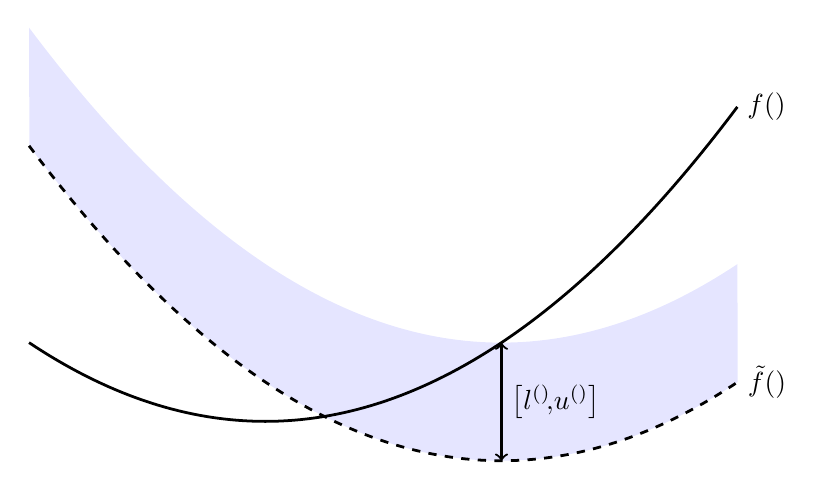
\begin{tikzpicture}[x=3cm, y=1cm]
					% Filled band around the quadratic curve with different boundary curves
					\fill[blue!10] 
					(-1, 5) -- plot[domain=-2:1, samples=100] ({\x+1}, {\x*\x + 1}) -- 
					plot[domain=1:-2, samples=100] ({\x+1}, {\x*\x - 0.5}) -- cycle;
					\node[anchor=west] at (2, 4) {$f(\weights)$};
					\draw[line width=1, domain=-2:1, samples=100,dashed] plot  ({\x+1}, {\x*\x -0.5}) node[right] {$\tilde{f}(\weights)$};
					\draw[line width=1, domain=-1:2, samples=100] plot ({\x}, {\x*\x});
					\draw[<->, thick] (1, -0.5) -- (1, 1) node[midway, right] {$\big[ l^{(\weights)}\!,\!u^{(\weights)} \big]$};
				\end{tikzpicture}
				\caption{Wir verwenden eine Schätzung $f(\weights)$ für das Leistungsmaß $\bar{f}(\weights)$ 
					um ein Konfidenzintervall $\big[ l^{(\weights)},  u^{(\weights)} \big]$ zu konstruieren. Ein Optimist 
					im Angesicht der Unsicherheit wählt Modellparameter $\weights$ gemäß dem günstigsten –
					 aber dennoch plausiblen – Wert $\tilde{f}(\weights) \defeq l^{(\weights)}$.} 
			\end{center}
	\end{figure}},first={Optimismus im Angesicht der Unsicherheit},text={Optimismus im Angesicht der Unsicherheit} 

\newglossaryentry{empgraph}
{
	name={Föderiertes Lernen Netzwerk (FL network)},
	description={Ein \gls{fl}-Netzwerk\index{federated learning network (FL network)} ist ein ungerichteter, 
	gewichteter \gls{graph}, dessen Knoten \gls{data}-Erzeuger repräsentieren, die lokale 
	(oder personalisierte) \gls{modelle} trainieren möchten. Jeder Knoten in einem \gls{fl}-Netzwerk steht 
	für ein \gls{device}, das in der Lage ist, ein \gls{localdataset} zu sammeln und daraus ein \gls{localmodel}
	 zu trainieren. \Gls{fl}-Methoden lernen für jeden Knoten $\nodeidx \in \nodes$ eine lokale \gls{hypothesis} $\localhypothesis{\nodeidx}$, 
	 sodass die \gls{loss} auf den jeweiligen \gls{localdataset}s minimiert wird.},
	first={föderiertes Lernen Netzwerk (FL network)},text={FL network} 
}


\newglossaryentry{norm}
{
	name={Norm},
	description={Eine \index{Norm} Norm ist eine Abbildung, die jedem (Vektor-)Element eines linearen Vektorraums 
	eine nicht-negative reelle Zahl zuordnet. Diese Abbildung muss homogen und definit sein sowie die Dreiecksungleichung 
	erfüllen \cite{HornMatAnalysis}.},
	first={Norm},text={Norm} 
}


\newglossaryentry{dualnorm}
{
	name={duale Norm},
	description={Jede \gls{norm} $\normgeneric{\cdot}{}$, definiert auf einem \gls{euclidspace} $\mathbb{R}^{\dimlocalmodel}$, besitzt eine zugehörige duale \gls{norm}, bezeichnet mit $\normgeneric{\cdot}{*}$ und definiert durch
		\[
		\normgeneric{\vy}{*} \defeq \sup_{\norm{\vx}{} \leq 1} \vy^{T} \vx.
		\]
		Die duale \gls{norm} misst das maximal mögliche Skalarprodukt zwischen $\vy$ und einem Vektor aus der Einheitskugel der ursprünglichen \gls{norm}. Weitere Details finden sich in \cite[Abschnitt A.1.6]{BoydConvexBook}.},
	first={duale Norm},
	text={duale Norm}
}

\newglossaryentry{geometricmedian}{
	name={geometrische Mitte (GM)},
	description={Die GM\index{geometrische Mitte (GM)} einer Menge von Eingabevektoren $\vx^{(1)}, \ldots, \vx^{(\samplesize)}$ 
		in $\mathbb{R}^{\dimlocalmodel}$ ist ein Punkt $\vz \in \mathbb{R}^{\dimlocalmodel}$, der 
		die Summe der Abstände zu diesen Vektoren minimiert \cite{BoydConvexBook}, d.\,h. 
		\begin{equation} 
			\label{equ_geometric_median}
			\vz \in \argmin_{\vy \in \mathbb{R}^{\dimlocalmodel}} \sum_{\sampleidx=1}^{\samplesize} \normgeneric{\vy - \vx^{(\sampleidx)}}{2}.
		\end{equation} 
		\begin{figure}[H]
			\begin{center}
				\begin{tikzpicture}[scale=2, thick, >=stealth]
					\coordinate (w) at (3,0);
					\fill (w) circle (1.2pt) node[below right] {$\vz$};
					\coordinate (w2) at (0.5,0.3);
					\coordinate (w3) at (0.7,0.7);
					\fill (w2) circle (1pt) node[above left] {$\vx^{(1)}$};
					\fill (w3) circle (1pt) node[above left] {$\vx^{(2)}$};
					\draw[dashed] (w) -- (w2);
					\draw[dashed] (w) -- (w3);
					\draw[->, thick, red] (w) -- ($(w)!1cm!(w2)$) ;
					\draw[->, thick, red] (w) -- ($(w)!1cm!(w3)$) node[pos=0.9, right,yshift=7pt] {$\frac{\vx^{(2)}- \vz}{\normgeneric{\vx^{(2)}-\vz}{2}}$};
					\coordinate (w4) at (5,0.2);
					\node at (5,0.4) {\textbf{Gestört}};
					\fill (w4) circle (1pt) node[below left] {$\vx^{(3)}$};
					\draw[->, thick, red] (w) -- ($(w)!1cm!(w4)$) ;
				\end{tikzpicture}
				\caption{\label{opt_cond_GM}
					Betrachte eine Lösung $\vz$ von \eqref{equ_geometric_median}, die nicht mit einem der Eingabevektoren übereinstimmt. 
					Die Optimalitätsbedingung für \eqref{equ_geometric_median} verlangt, dass die Einheitsvektoren von $\vz$ zu den Eingabevektoren 
					in der Summe null ergeben.}
			\end{center}
		\end{figure}
		Abbildung~\ref{opt_cond_GM} illustriert eine fundamentale Eigenschaft der GM:
		Falls $\vz$ nicht mit einem der Eingabevektoren übereinstimmt, müssen die Einheitsvektoren, 
		die von $\vz$ zu jedem $\vx^{(\sampleidx)}$ zeigen, in der Summe null ergeben — dies ist die 
		Null-\gls{subgradient}- (Optimalitäts-) Bedingung von \eqref{equ_geometric_median}. 
		Es zeigt sich, dass die Lösung von \eqref{equ_geometric_median} nicht beliebig weit von den vertrauenswürdigen 
		Eingabevektoren weggezogen werden kann, solange diese die Mehrheit bilden \cite[Th. 2.2]{Lopuhaae1991}.},
	first={geometrische Mitte},
	text={GM}
}

\newglossaryentry{explanation}
{name={Erklärung},
	description={Ein Ansatz, um \gls{ml}-Methoden transparenter zu machen, besteht darin, 
		eine Erklärung\index{Erklärung} zusammen mit der von einer \gls{ml}-Methode gelieferten 
		\gls{prediction} bereitzustellen. Erklärungen können in unterschiedlichen Formen auftreten. 
		Eine Erklärung kann beispielsweise ein natürlichsprachlicher Text sein oder eine quantitative 
		Maßzahl, welche die Bedeutung einzelner \gls{feature}s eines \gls{datapoint}s beschreibt \cite{Molnar2019}. 
		Es können auch visuelle Formen von Erklärungen genutzt werden, etwa Intensitätskarten bei der Bild-\gls{classification} \cite{GradCamPaper}.},
	first={Erklärung},text={Erklärung} 
}

\newglossaryentry{risk}
{name={Risiko},
	description={Betrachte\index{Risiko} eine \gls{hypothesis} $\hypothesis$, die verwendet wird, um das \gls{label} 
		$\truelabel$ eines \gls{datapoint} auf Basis seiner \gls{feature}s $\featurevec$ vorherzusagen. 
		Die Qualität einer bestimmten \gls{prediction} wird mithilfe einer \gls{lossfunc} 
		$\lossfunc{(\featurevec,\truelabel)}{\hypothesis}$ gemessen. Wenn wir \gls{datapoint}s als 
		\gls{realization}en von \glspl{rv} interpretieren, die \gls{iid} sind, dann wird auch 
		$\lossfunc{(\featurevec,\truelabel)}{\hypothesis}$ zur \gls{realization} einer \gls{rv}. 
		Die Annahme der \gls{iidasspt} erlaubt es uns, das Risiko einer \gls{hypothesis} als den erwarteten 
		\gls{loss} zu definieren: $\expect \big\{\lossfunc{(\featurevec,\truelabel)}{\hypothesis} \big\}$. 
		Beachte, dass das Risiko von $\hypothesis$ sowohl von der konkreten Wahl der \gls{lossfunc} 
		als auch von der \gls{probdist} der \gls{datapoint}s abhängt.},
	first={Risiko},text={Risiko}, plural={Risiken}
}

\newglossaryentry{actfun}
{name={Aktivierungsfunktion},
	description={Jedem\index{Aktivierungsfunktion} künstlichen Neuron innerhalb eines \gls{ann} 
		wird eine Aktivierungsfunktion $\actfun(\cdot)$ zugewiesen, die eine gewichtete 
		Kombination der Neuronen-Eingaben $\feature_{1},\ldots,\feature_{\nrfeatures}$ 
		auf einen einzelnen Ausgabewert abbildet: 
		$a = \actfun\big(\weight_{1} \feature_{1}+\ldots+\weight_{\nrfeatures} \feature_{\nrfeatures} \big)$. 
		Jedes Neuron ist dabei durch die \glspl{weights} $\weight_{1},\ldots,\weight_{\nrfeatures}$ parametrisiert.},
	first={Aktivierungsfunktion},text={Aktivierungsfunktion} , plural={Aktivierungsfunktionen}
}

\newglossaryentry{distributedalgorithm}
{name={verteiltes Algorithmusverfahren},
	description={Ein\index{verteiltes Algorithmusverfahren} verteiltes \gls{algorithmus}verfahren ist ein \gls{algorithmus}, 
		der für eine spezielle Art von Rechensystemen entwickelt wurde, nämlich für eine Sammlung 
		interagierender Rechengeräte (sogenannte Knoten). Diese Knoten kommunizieren und koordinieren 
		ihre lokalen Berechnungen durch den Austausch von Nachrichten über ein Netzwerk 
		\cite{IntroDistAlg}, \cite{ParallelDistrBook}. Im Gegensatz zu einem klassischen \gls{algorithmus}, 
		der auf einem einzelnen \gls{device} ausgeführt wird, läuft ein verteiltes \gls{algorithmus}verfahren 
		gleichzeitig auf mehreren \gls{device}s mit eigener Rechenkapazität ab. 
		
		Ähnlich wie ein klassischer \gls{algorithmus} lässt sich auch ein verteiltes Verfahren als 
		Menge möglicher Ausführungsverläufe modellieren. Allerdings beinhalten die Ausführungen im 
		verteilten Fall sowohl lokale Berechnungen als auch Kommunikationsereignisse. 
		Eine typische Ausführung könnte folgendermaßen aussehen:
		\[
		\begin{array}{l}
			\text{Knoten 1: } {\rm input}_1, s_1^{(1)}, s_2^{(1)}, \ldots, s_{T_1}^{(1)}, {\rm output}_1; \\
			\text{Knoten 2: } {\rm input}_2, s_1^{(2)}, s_2^{(2)}, \ldots, s_{T_2}^{(2)}, {\rm output}_2; \\
			\quad \vdots \\
			\text{Knoten N: } {\rm input}_N, s_1^{(N)}, s_2^{(N)}, \ldots, s_{T_N}^{(N)}, {\rm output}_N.
		\end{array}
		\]
		Jedes \gls{device} $\nodeidx$ beginnt mit einem eigenen lokalen Eingabewert und führt eine Sequenz 
		von Zwischenrechnungen $s_{\iteridx}^{(\nodeidx)}$ zu diskreten Zeitpunkten $\iteridx = 1, \dots, T_\nodeidx$ durch. 
		Diese Berechnungen können sowohl von vorherigen lokalen Berechnungsschritten als auch von empfangenen 
		Nachrichten anderer \gls{device}s abhängen. 
		
		Eine wichtige Anwendung verteilter \glspl{algorithmus} ist das \gls{fl}, bei dem ein Netzwerk 
		von \glspl{device} kollaborativ ein persönliches \gls{model} für jedes \gls{device} trainiert.},
	first={verteiltes Algorithmusverfahren}, text={verteiltes Algorithmusverfahren}
}

\newglossaryentry{algorithm}
{name={Algorithmus},
	description={Ein\index{Algorithmus} Algorithmus ist eine präzise, schrittweise Vorschrift, 
		wie aus einer gegebenen Eingabe in endlich vielen Rechenschritten eine Ausgabe erzeugt wird \cite{Cormen:2022aa}. 
		Ein Beispiel ist ein Algorithmus zum Trainieren eines \gls{linmodel}, der explizit beschreibt, 
		wie ein gegebenes \gls{trainset} durch eine Folge von \glspl{gradstep} in \glspl{modelparams} 
		transformiert wird. 
		
		Diese informelle Beschreibung lässt sich durch verschiedene mathematische \gls{model}le 
		rigide formalisieren \cite{Sipser2013}. Ein einfaches \gls{model} eines Algorithmus ist 
		die Menge möglicher Ausführungen, wobei jede Ausführung eine Folge der Form
		$${\rm input},s_1,s_2,\ldots,s_T,{\rm output}$$
		darstellt, die den Beschränkungen der zugrunde liegenden Rechenarchitektur genügt.
		
		Algorithmen können \emph{deterministisch} sein, sodass jede Eingabe zu einer eindeutig bestimmten 
		Ausführung führt, oder \emph{randomisiert}, wobei sich Ausführungen mit gewisser Wahrscheinlichkeit 
		unterscheiden. Randomisierte Algorithmen lassen sich daher durch stochastische Prozesse analysieren, 
		wobei Ausführungsfolgen als Ergebnisse zufälliger Experimente modelliert werden 
		\cite{BertsekasProb}, \cite{RandomizedAlgos}, \cite{Gallager13}.
		
		Wesentlich ist, dass ein Algorithmus mehr umfasst als lediglich eine Abbildung von Eingabe 
		auf Ausgabe: Auch die Zwischenschritte $s_1,\ldots,s_T$ gehören zur vollständigen Beschreibung des Verfahrens.},
	first={Algorithmus},text={Algorithmus}, plural={Algorithmen}
}

\newglossaryentry{stochalgorithm}
{name={stochastischer Algorithmus}, 
 plural={stochastische Algorithmen},
	description={Ein\index{stochastischer Algorithmus} \gls{stochastischer} \gls{Algorithmus} nutzt während seiner Ausführung einen Zufallsmechanismus. 
		Beispielsweise verwendet \gls{stochGD} eine zufällig ausgewählte Teilmenge von \glspl{datapoint}, 
		um eine Näherung für den \gls{gradient} einer \gls{objfunc} zu berechnen. 
		Wir können einen \gls{stochastischen} \gls{Algorithmus} durch einen \glspl{stochproc} darstellen, 
		d. h., die möglichen Ausführungsfolgen entsprechen den möglichen Ergebnissen eines 
		\gls{randomexperiment} \cite{BertsekasProb}, \cite{RandomizedAlgos}, \cite{Gallager13}.		
		\\ 
		Siehe auch: \gls{stochastic}, \gls{algorithm}, \gls{stochGD}, \gls{datapoint}, \gls{gradient}, \gls{objfunc}, \gls{stochproc}, 
		\gls{randomexperiment}, \gls{optmethod}, \gls{gdmethod}. },
	first={stochastischer Algorithmus},
	text={stochastischer Algorithmus} 
}

\newglossaryentry{batchlearning}
{name={Batch-Lernen},
	description={Beim \gls{batch} Lernen\index{Batch-Lernen} (auch als Offline-Lernen bekannt) wird das \gls{ml} \gls{model} 
		auf dem gesamten \gls{dataset} in einer einzigen Trainingsiteration trainiert, anstatt es inkrementell zu aktualisieren, sobald neue \gls{data} eintreffen. 
		Alle verfügbaren \gls{data} werden in einen Lern-\gls{algorithm} eingespeist, wodurch ein \gls{model} entsteht, das \glspl{prediction} liefern kann. 
		Da diese \glspl{dataset} oft groß sind, ist das Training rechenaufwendig und zeitintensiv und wird daher typischerweise offline durchgeführt. 
		Nach dem Lernen ist das \gls{model} statisch und passt sich nicht automatisch an neue \gls{data} an. 
		Ein Aktualisieren des \gls{model} mit neuen Informationen erfordert ein vollständiges Retraining. 
		Sobald das \gls{model} trainiert ist, wird es in die Produktion gebracht, wo es nicht aktualisiert werden kann. 
		Da das Training eines \gls{model} viele Stunden dauern kann, werden viele \glspl{model} in Produktionsumgebungen zyklisch nach einem festen Zeitplan aktualisiert, 
		wenn die \gls{data}-Verteilung stabil ist. Beispielsweise könnte ein Einzelhandels-Analytics-Team ihr Nachfrageprognose-\gls{model} jeden Sonntag 
		mit den Verkaufsdaten der Vorwoche neu trainieren, um die Nachfrage der nächsten Woche vorherzusagen. 
		Falls ein System kontinuierlich an schnell ändernde \gls{data} angepasst werden muss, wie z. B. bei der Vorhersage von Aktienkursen, 
		ist eine anpassungsfähigere Lösung wie \gls{onlinelearning} erforderlich.
		\\
		Siehe auch: \gls{batch}, \gls{model}, \gls{dataset}, \gls{onlinelearning}. },
	first={Batch-Lernen}, 
	text={Batch-Lernen}
}

\newglossaryentry{onlinelearning}
{name={Online-Lernen},
	description={Einige \gls{ml}-Methoden\index{Online-Lernen} sind darauf ausgelegt, \gls{data} 
		sequentiell zu verarbeiten und ihre \glspl{modelparam} jeweils einzeln zu aktualisieren, sobald neue \glspl{datapoint} verfügbar werden. 
		Ein typisches Beispiel sind Zeitreihen-\gls{data}, wie tägliche \gls{minimum}- und \gls{maximum}-Temperaturen, 
		die von einer \gls{fmi}-Wetterstation aufgezeichnet werden. Diese Werte bilden eine chronologische Folge von Beobachtungen. 
		In jedem Zeitschritt $\timeidx$ aktualisieren (oder verfeinern) Online-Lernmethoden die aktuelle \gls{hypothesis} 
		$\hypothesis^{(\timeidx)}$ (oder \glspl{modelparam} $\weights^{(\timeidx)}$) basierend auf dem neu beobachteten \gls{datapoint} 
		$\datapoint^{(\timeidx)}$.
		\\ 
		Siehe auch: \gls{onlineGD}, \gls{onlinealgorithm}. },
	first={Online-Lernen},
	text={Online-Lernen}
}


\newglossaryentry{onlinealgorithm}
{name={Online-Algorithmus},
	description={Ein\index{Online-Algorithmus} Online-\gls{algorithmus} verarbeitet Eingabedaten inkrementell, 
		indem die \gls{data} schrittweise empfangen und unmittelbar verarbeitet werden, 
		d.h. Entscheidungen oder Ausgaben erfolgen sofort, ohne dass der gesamte Eingabestrom im Voraus bekannt ist 
		\cite{PredictionLearningGames}, \cite{HazanOCO}. 
		
		Im Gegensatz zu einem Offline-\gls{algorithmus}, der von Anfang an Zugriff auf die vollständige Eingabe hat, 
		muss ein Online-\gls{algorithmus} mit der \gls{uncertainty} zukünftiger Eingaben umgehen und kann frühere 
		Entscheidungen nicht revidieren. Ähnlich wie ein Offline-\gls{algorithmus} lässt sich ein Online-\gls{algorithmus} 
		formal als Menge möglicher Ausführungsverläufe modellieren. Die Struktur einer Ausführung unterscheidet sich jedoch 
		grundlegend und folgt dem Schema:
		\[
		{\rm in}_{1},s_1,{\rm out}_{1},{\rm in}_{2},s_2,{\rm out}_{2},\ldots,{\rm in}_{T},s_T,{\rm out}_{T}.
		\]
		Jede Ausführung beginnt mit einem initialen Zustand (\({\rm in}_{1}\)) und besteht aus abwechselnden 
		Rechenschritten, Ausgaben (oder Entscheidungen) und neu eingehenden Daten. 
		Im Schritt \(\iteridx\) führt der \gls{algorithmus} eine Berechnung \(s_{\iteridx}\) aus, 
		erzeugt eine Ausgabe \({\rm out}_{\iteridx}\) und erhält anschließend die nächste Eingabe \({\rm in}_{\iteridx+1}\). 
		
		Ein bekanntes Beispiel für einen Online-\gls{algorithmus} im Bereich \gls{ml} ist der 
		\gls{onlineGD}, bei dem \glspl{modelparams} schrittweise aktualisiert werden, sobald neue 
		\glspl{datapoint} eintreffen.},
	first={Online-Algorithmus},text={Online-Algorithmus} 
}

\newglossaryentry{transparency}
{name={Transparenz},
	description={Transparenz\index{Transparenz} ist eine grundlegende Voraussetzung für 
		\gls{trustAI} \cite{HLEGTrustworhtyAI}. Im Kontext von \gls{ml}-Methoden wird Transparenz 
		oft synonym mit \gls{explainability} verwendet \cite{JunXML2020}, \cite{gallese2023ai}. 
		Im weiteren Sinne von \gls{ai}-Systemen umfasst Transparenz jedoch mehr als nur 
		Erklärbarkeit: Sie beinhaltet auch die Offenlegung von Beschränkungen, Zuverlässigkeit 
		und dem beabsichtigten Einsatzgebiet des Systems. 
		
		In medizinischen Diagnosesystemen bedeutet Transparenz etwa die Angabe der Vertrauenswürdigkeit 
		der vom trainierten \gls{model} gelieferten \gls{prediction}en. Im Bereich der Kreditvergabe 
		sollten \gls{ai}-basierte Entscheidungen durch Erklärungen der relevanten Einflussfaktoren 
		– etwa Einkommen oder Kreditgeschichte – begleitet werden. Diese Erklärungen ermöglichen es 
		den Betroffenen, etwa Kreditnehmern, die automatisierten Entscheidungen nachzuvollziehen und anzufechten. 
		
		Einige \gls{ml}-Methoden bieten von Natur aus Transparenz: So liefert \gls{logreg} 
		eine quantitative Abschätzung der Zuverlässigkeit einer \gls{classification} über den Wert $|\hypothesis(\featurevec)|$. 
		\Gls{decisiontree}s sind ein weiteres Beispiel, da sie gut verständliche Entscheidungsregeln 
		bieten \cite{rudin2019stop}.
		
		Transparenz verlangt zudem eine klare Kennzeichnung, wenn ein Benutzer mit einem \gls{ai}-System interagiert. 
		Beispielsweise sollten \gls{ai}-gestützte Chatbots ihre Nutzer darüber informieren, dass sie mit einem automatisierten 
		System und nicht mit einem Menschen kommunizieren. 
		
		Darüber hinaus umfasst Transparenz eine umfassende Dokumentation, welche Zweck, Designentscheidungen 
		und vorgesehenen Einsatzbereiche des \gls{ai}-Systems erläutert. Beispielhaft sind hier 
		\gls{model}-Datasheets \cite{DatasheetData2021} und \gls{ai}-System-Cards \cite{10.1145/3287560.3287596}, 
		die Praktiker:innen helfen, die Einsatzmöglichkeiten und Grenzen eines \gls{ai}-Systems zu verstehen \cite{Shahriari2017}.},
	first={Transparenz}, text={Transparenz} 
}

\newglossaryentry{sensattr}
{
	name={sensitive Attribut},
	description={
		\gls{ml}\index{sensitive Attribut} bezeichnet das Gebiet des maschinellen Lernens, bei dem eine \gls{Hypothese}-Funktion erlernt wird, die es ermöglicht, das \gls{Label} eines \gls{Datenpunkts} anhand seiner \gls{Merkmale} vorherzusagen. In bestimmten Anwendungsfällen muss sichergestellt werden, dass die Ausgabe eines \gls{ML}-Modells keine Rückschlüsse auf sensitive Attribute eines \gls{Datenpunkts} zulässt. Welche Merkmale eines \gls{Datenpunkts} als sensitive Attribute klassifiziert werden, ist eine kontextspezifische Designentscheidung und variiert je nach Anwendungsgebiet.
	},
	first={sensitive Attribut},
	text={sensitive Attribut}, plural={sensitive Attribute}
}


\newglossaryentry{sbm}
{
	name={stochastisches Blockmodell (SBM)},
	description={
		Das\index{stochastisches Blockmodell (SBM)} stochastische Block-\gls{modell} ist ein probabilistisches generatives \gls{modell} für einen ungerichteten \gls{graph} $\graph = \big( \nodes, \edges \big)$ 
		mit einer gegebenen Menge von Knoten $\nodes$ \cite{AbbeSBM2018}. In seiner einfachsten Variante 
		generiert das stochastische Block-\gls{modell} einen \gls{graph}, indem zunächst jeder Knoten $\nodeidx \in \nodes$ 
		zufällig einem \gls{cluster}-Index $\clusteridx_{\nodeidx} \in \{1,\ldots,\nrcluster\}$ zugeordnet wird. 
		Ein Paar verschiedener Knoten im \gls{graph} wird mit einer \gls{wahrscheinlichkeit} $p_{\nodeidx,\nodeidx'}$ verbunden, 
		die ausschließlich von den \gls{label}n $\clusteridx_{\nodeidx}, \clusteridx_{\nodeidx'}$ abhängt. 
		Das Vorhandensein von Kanten zwischen verschiedenen Knotenpaaren ist statistisch unabhängig.
	},
	first={stochastisches Blockmodell (SBM)},
	text={SBM}
}

\newglossaryentry{deepnet}
{
	name={Deep Net},
	description={
		Ein\index{Deep Net} Deep Net ist ein \gls{ANN} mit einer (relativ) großen Anzahl von 
		versteckten Schichten. Deep Learning ist ein Oberbegriff für \gls{ML}-Methoden, die ein Deep Net als ihr \gls{Modell} verwenden \cite{Goodfellow-et-al-2016}.
	},
	first={Deep Net},
	text={Deep Net}
}


\newglossaryentry{baseline}
{
	name={Baseline},
	description={
		Betrachte\index{Baseline} eine \gls{ML}-Methode, die eine gelernte \gls{Hypothese} (bzw. ein trainiertes \gls{Modell}) $\learnthypothesis \in \hypospace$ liefert. Die Qualität eines trainierten \gls{Modells} wird häufig über den durchschnittlichen \gls{Loss} auf einem \gls{Testset} bewertet. Doch wie lässt sich beurteilen, ob die erzielte Leistung auf dem \gls{Testset} ausreichend gut ist? Wie kann man feststellen, ob das trainierte \gls{Modell} nahezu optimal arbeitet und es wenig sinnvoll ist, weitere Ressourcen (für \gls{Daten}sammlung oder Berechnung) in eine Verbesserung zu investieren? 
		
		Zu diesem Zweck ist es hilfreich, einen Referenz- oder Baseline-Wert zu haben, mit dem die Leistung des trainierten \gls{Modells} verglichen werden kann. Ein solcher Referenzwert kann beispielsweise aus menschlicher Leistung gewonnen werden, etwa der Fehlklassifikationsrate von Dermatologen, die Krebs durch visuelle Hautinspektion diagnostizieren \cite{SkinHumanAI}. Eine weitere Quelle für eine Baseline ist eine bestehende, aber aus bestimmten Gründen ungeeignete \gls{ML}-Methode. Beispielsweise könnte diese Methode für die geplante Anwendung zu rechenintensiv sein. Dennoch kann deren Fehler auf dem \gls{Testset} als Baseline dienen.
		
		Ein etwas prinzipiellerer Ansatz zur Konstruktion einer Baseline basiert auf einem \gls{Probmodell}. In vielen Fällen lässt sich für ein gegebenes \gls{Probmodell} $p(\featurevec,\truelabel)$ das minimal erreichbare \gls{Risk} unter allen Hypothesen exakt bestimmen (wobei diese nicht zwingend zum \gls{Hypothesenraum} $\hypospace$ gehören müssen) \cite{LC}. Dieses minimal erreichbare \gls{Risk} (bekannt als \gls{Bayesrisk}) entspricht dem \gls{Risk} des \gls{Bayesestimator} für das \gls{Label} $\truelabel$ eines \gls{Datenpunkts} mit \gls{Features} $\featurevec$. Dabei ist zu beachten, dass für eine gegebene Wahl der \gls{Lossfunktion} der \gls{Bayesestimator} (sofern er existiert) vollständig durch die \gls{Wahrscheinlichkeitsverteilung} $p(\featurevec,\truelabel)$ bestimmt ist \cite[Kap. 4]{LC}. 
		
		Die Berechnung von \gls{Bayesestimator} und \gls{Bayesrisk} stellt jedoch zwei zentrale Herausforderungen dar:
		\begin{enumerate}[label=\arabic*)]
			\item Die \gls{Wahrscheinlichkeitsverteilung} $p(\featurevec,\truelabel)$ ist in der Regel unbekannt und muss geschätzt werden.
			\item Selbst wenn $p(\featurevec,\truelabel)$ bekannt ist, kann die exakte Berechnung des \gls{Bayesrisk} rechnerisch zu aufwendig sein \cite{cooper1990computational}.
		\end{enumerate}
		
		Ein weit verbreitetes \gls{Probmodell} ist die \gls{MVNDist} $\pair{\featurevec}{\truelabel} \sim \mathcal{N}({\bm \mu},{\bm \Sigma})$ für \gls{Datenpunkte}, die durch numerische \gls{Features} und \gls{Labels} charakterisiert sind. Für die \gls{SQErrLoss} ist der \gls{Bayesestimator} in diesem Fall der bedingte Mittelwert $\mu_{\truelabel|\featurevec}$ des \gls{Labels} $\truelabel$ gegeben die \gls{Features} $\featurevec$ \cite{LC}, \cite{GrayProbBook}. Das zugehörige \gls{Bayesrisk} entspricht der posterioren Varianz $\sigma^{2}_{\truelabel|\featurevec}$ (siehe Abb. \ref{fig_post_baseline_dict}).
		
		\begin{figure}[H]
			\begin{center}
				\begin{tikzpicture}
					% Achsen
					\draw[->] (-1,0) -- (7,0) node[right] {$\truelabel$}; % x-Achse
					% Gaußsche Verteilung zentriert bei \gaussiancenter mit Varianz 1
					\draw[thick,domain=-1:7,smooth,variable=\x] 
					plot ({\x}, {2*exp(-0.5*((\x-\gaussiancenter)^2))});
					% Gestrichelte Linie für Mittelwert der Gaußverteilung
					\draw[dashed] (\gaussiancenter,0) -- (\gaussiancenter,2.5);
					\node[anchor=south] at ([yshift=-5pt] \gaussiancenter,2.5) {\small $\mu_{\truelabel|\featurevec}$};
					% Doppelpfeil für Varianz
					\draw[<->,thick] (\gaussiancenter-1,1) -- (\gaussiancenter+1,1.0);
					\node[anchor=west] at ([yshift=2pt] \gaussiancenter,1.2) {\small $\sigma_{\truelabel|\featurevec}$};
					% Markierung der x-Achse mit Kreuz
					\foreach \x in {0.5} {
						\node[red] at (\x, 0) {\bf \large $\times$};
					}
					% Beschriftung für erstes Kreuz
					\node[anchor=north] at (0.5,-0.2) {\small $\learnthypothesis(\featurevec)$};
				\end{tikzpicture}
			\end{center}
			\caption{Sind die \gls{Features} und das \gls{Label} eines \gls{Datenpunkts} gemäß einer \gls{MVNDist} verteilt, so lässt sich das minimale \gls{Risk} (unter \gls{SQErrLoss}) durch den \gls{Bayesestimator} $\mu_{\truelabel|\featurevec}$ erzielen, der das \gls{Label} $\truelabel$ anhand der \gls{Features} $\featurevec$ vorhersagt. Das zugehörige minimale \gls{Risk} entspricht der posterioren Varianz $\sigma^{2}_{\truelabel|\featurevec}$. Diese Größe kann als Baseline für den durchschnittlichen \gls{Loss} eines trainierten \gls{Modells} $\learnthypothesis$ verwendet werden.\label{fig_post_baseline_dict}}
		\end{figure}
	},
	first={Baseline},
	text={Baseline}
}

\newglossaryentry{kfoldcv}
{name={$k$-fach Kreuzvalidierung ($k$-fold CV)},
 description={Eine Methode\index{$k$-fach Kreuzvalidierung} zur Bewertung der 
 \gls{gengap} eines \gls{erm}-basierten \gls{ml}-Verfahrens. Die Idee besteht darin, 
 das \gls{dataset} $\dataset$ gleichmäßig in $k$ Teilmengen (oder Folds) 
 $\dataset^{(1)},\ldots,\dataset^{(k)}$ zu unterteilen.
	\begin{figure}[htbp]
		\centering
	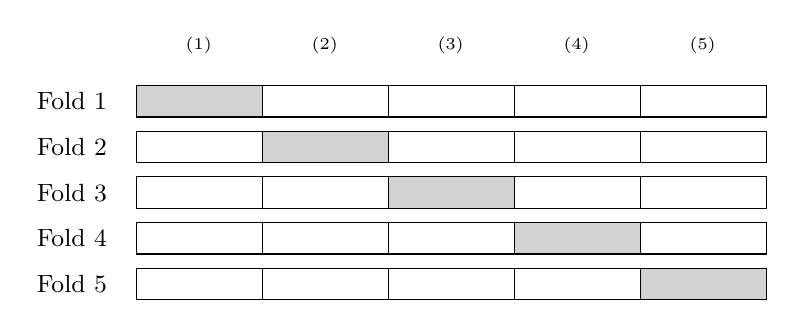
\begin{tikzpicture}[font=\small]
		\def\k{5}          % number of folds
		\def\cellw{1.6}    % width of one segment
		\def\cellh{0.40}   % height of one segment
		\def\gap{0.18}     % vertical gap between rows
		% rows: i = 1..k; columns: j = 1..k
		\foreach \i in {1,...,\k} {
			% row baseline y
			\pgfmathsetmacro{\y}{-(\i-1)*(\cellh+\gap)}
			% row label
			\node[anchor=east] at (-0.25,\y+0.5*\cellh) {Fold \i};
			% draw k equal segments; shade the \i-th as validation
			\foreach \j in {1,...,\k} {
				\pgfmathsetmacro{\x}{(\j-1)*\cellw}
				\ifnum\i=\j
				\fill[gray!35] (\x,\y) rectangle ++(\cellw,\cellh);
				\draw (\x,\y) rectangle ++(\cellw,\cellh);
				\else
				\draw (\x,\y) rectangle ++(\cellw,\cellh);
				\fi
			}
		}
		% add labels D^{(j)} above the columns
		\foreach \j in {1,...,\k} {
			\pgfmathsetmacro{\x}{(\j-1)*\cellw + 0.5*\cellw}
			\node[anchor=south] at (\x,\cellh+0.2) {$\dataset^{(\j)}$};
		}
	\end{tikzpicture}
	\caption{Bei der $k$-fach Kreuzvalidierung wird das verfügbare \gls{dataset} $\dataset$ 
	gleichmäßig in $k$ Folds $\dataset^{(1)},\ldots,\dataset^{(k)}$ unterteilt. 
	Jeder Fold wird einmal als \gls{valset} verwendet, während die verbleibenden $k-1$ Folds 
	das \gls{trainset} bilden.		
	\label{fig_kfoldcv_dict}}
	\end{figure} 
	Für jeden Fold $\foldidx = 1, \,\ldots, \,k$ wird das \gls{model} auf der Vereinigung 
	aller Folds außer $\dataset^{(\foldidx)}$ trainiert und auf 
	$\dataset^{(\foldidx)}$ validiert. Die Gesamtleistung ergibt sich durch Mittelung 
	der \gls{validation}-Ergebnisse über alle $k$ Folds.
	\\ 
	Siehe auch: \gls{validation}, \gls{valerr}.},
	first={$k$-fach Kreuzvalidierung ($k$-fold CV)},
	text={$k$-fold CV} 
}


\newglossaryentry{spectrogram}
{
	name={Spektrogramm},
	description={
		Ein\index{Spektrogramm} Spektrogramm beschreibt die Zeit-Frequenz-Verteilung der Energie eines Zeitsignals $x(t)$. Anschaulich quantifiziert es, wie viel Signalenergie in einem bestimmten Zeitintervall 
		$[t_{1}, t_{2}] \subseteq \mathbb{R}$ und Frequenzbereich $[f_{1}, f_{2}] \subseteq \mathbb{R}$ enthalten ist. 
		
		Formal ist das Spektrogramm eines Signals definiert als das Quadrat des Betrags seiner Kurzzeit-Fourier-Transformation (STFT, short-time Fourier transform) \cite{cohen1995time}.
		
		Abbildung \ref{fig:spectrogram_dict} zeigt ein Zeitsignal zusammen mit seinem Spektrogramm.
		
		\begin{figure}[H]
			\centering
			\includegraphics[width=0.8\textwidth]{assets/spectrogram.png}
			\caption{Links: Ein Zeitsignal bestehend aus zwei modulierten Gauß-Pulsen. Rechts: Ein Intensitätsdiagramm des zugehörigen Spektrogramms.
				\label{fig:spectrogram_dict}}
		\end{figure}
		
		Das Intensitätsbild eines Spektrogramms kann als Bildrepräsentation eines Signals dienen. Ein einfaches Verfahren zur \gls{Klassifikation} von Audiosignalen besteht darin, dieses Signalbild in \gls{DeepNet}s einzuspeisen, die ursprünglich für die Bild-\gls{Klassifikation} und Objekterkennung entwickelt wurden \cite{Li:2022aa}.
		
		Es sei angemerkt, dass es neben dem Spektrogramm noch zahlreiche alternative Darstellungen zur Beschreibung der Zeit-Frequenz-Verteilung der Signalenergie gibt \cite{TimeFrequencyAnalysisBoashash}, \cite{MallatBook}.
	},
	first={Spektrogramm},
	text={Spektrogramm}, plural={Spektogramme}
}

\newglossaryentry{graphclustering}
{
	name={Graph-Clustering},
	description={
		\Gls{Graph}-\gls{Clustering}\index{Graph-Clustering} bezeichnet das \gls{Clustering} von \gls{Datenpunkten}, 
		die als Knoten eines \gls{Graphen} $\graph$ repräsentiert werden. Die Kanten von $\graph$ 
		spiegeln paarweise Ähnlichkeiten zwischen den \gls{Datenpunkten} wider. In manchen Fällen 
		lassen sich diese Ähnlichkeiten durch ein \gls{Kantengewicht} quantitativ beschreiben \cite{FlowSpecClustering2021}, \cite{Luxburg2007}.
	},
	first={Graph-Clustering},
	text={Graph-Clustering}
}


\newglossaryentry{specclustering}
{
	name={Spektrales Clustering},
	description={
		Das spektrale \gls{Clustering}\index{Spektrales Clustering} ist eine spezielle Methode des \gls{GraphClustering}, 
		bei der \gls{Datenpunkte} geclustert werden, die durch die Knoten $\nodeidx = 1, \ldots, \nrnodes$ eines 
		\gls{Graphen} $\graph$ dargestellt werden. 
		
		Beim spektralen \gls{Clustering} werden die \gls{Eigenvektoren} der \gls{LapMat} $\LapMat{\graph}$ verwendet, 
		um \gls{Featurevektoren} $\featurevec^{(\nodeidx)} \in \mathbb{R}^{\nrfeatures}$ für jeden Knoten (also jeden \gls{Datenpunkt}) 
		$\nodeidx=1,\ldots,\nrnodes$ zu konstruieren. Diese \gls{Featurevektoren} können anschließend als Eingabe für 
		\gls{Clustering}-Methoden im \gls{Euklidischen Raum} verwendet werden, z.\,B. \gls{KMeans} oder \gls{SoftClustering} mittels \gls{GMM}. 
		
		Grob gesagt liegen die \gls{Featurevektoren} der Knoten, die zu einer gut verbundenen Teilmenge 
		(also einem \gls{Cluster}) in $\graph$ gehören, im \gls{Euklidischen Raum} $\mathbb{R}^{\nrfeatures}$ nahe beieinander 
		(siehe Abb.~\ref{fig_lap_mtx_specclustering_dict}).
		
		\begin{figure}[H]
			\begin{center}
				\begin{minipage}{0.4\textwidth}
					\begin{tikzpicture}
						\begin{scope}[every node/.style={circle, fill=black, inner sep=0pt, minimum size=0.3cm}]
							\node (1) at (0,0) {};
							\node (2) [below left=of 1, xshift=-0.2cm, yshift=-1cm] {};
							\node (3) [below right=of 1, xshift=0.2cm, yshift=-1cm] {};
							\node (4) [below=of 1, yshift=0.5cm] {};
						\end{scope}
						\draw (1) -- (2);
						\draw (1) -- (3);
						\node[above=0.2cm] at (1) {$\nodeidx=1$};
						\node[left=0.3cm] at (2) {$2$};
						\node[right=0.3cm] at (3) {$3$};
						\node[below=0.2cm] at (4) {$4$};
					\end{tikzpicture}
				\end{minipage}
				\hspace*{5mm}
				\begin{minipage}{0.4\textwidth}
					\begin{equation} 
						\LapMat{\graph} =
						\begin{pmatrix} 
							2 & -1 & -1 & 0 \\ 
							-1 & 1 & 0 & 0 \\  
							-1 & 0 & 1 & 0 \\ 
							0 & 0 & 0 & 0 
						\end{pmatrix}
						= \mathbf{V} {\bm \Lambda} \mathbf{V}^{T}
						\nonumber
					\end{equation}
				\end{minipage}
				\vspace*{20mm}\\
				\begin{minipage}{0.4\textwidth}
					\begin{tikzpicture}[scale=3]
						\draw[->] (-0.2, 0) -- (1.2, 0) node[right] {$v^{(1)}_{\nodeidx}$};
						\draw[->] (0, -0.2) -- (0, 1.2) node[above] {$v^{(2)}_{\nodeidx}$};
						\filldraw[blue] (0.577, 0) circle (0.03cm) node[above right] {$\nodeidx=1,2,3$};
						\filldraw[blue] (0.577, 0) circle (0.03cm);
						\filldraw[blue] (0.577, 0) circle (0.03cm);
						\filldraw[red] (0, 1) circle (0.03cm) node[above right] {$4$};
					\end{tikzpicture}
				\end{minipage}
				\begin{minipage}{0.4\textwidth}
					\begin{align}
						& \mathbf{V} = \big( \vv^{(1)},\vv^{(2)},\vv^{(3)},\vv^{(4)} \big) \nonumber \\
						& \mathbf{v}^{(1)} = \frac{1}{\sqrt{3}} \begin{pmatrix} 1 \\ 1 \\ 1 \\ 0 \end{pmatrix}, \quad
						\mathbf{v}^{(2)} = \begin{pmatrix} 0 \\ 0 \\ 0 \\ 1 \end{pmatrix} \nonumber
					\end{align}
				\end{minipage}
				\caption{\label{fig_lap_mtx_specclustering_dict} 
					{\bf Oben.} Links: Ein ungerichteter \gls{Graph} $\graph$ mit vier Knoten $\nodeidx=1,2,3,4$, 
					die jeweils einen \gls{Datenpunkt} repräsentieren. Rechts: Die \gls{LapMat} 
					$\LapMat{\graph} \in \mathbb{R}^{4 \times 4}$ und ihre \gls{EVD}. 
					{\bf Unten.} Links: Ein \gls{Streudiagramm} der \gls{Datenpunkte} mithilfe der 
					\gls{Featurevektoren} $\featurevec^{(\nodeidx)} = \big( v^{(1)}_{\nodeidx}, v^{(2)}_{\nodeidx} \big)^T$. 
					Rechts: Zwei \gls{Eigenvektoren} $\vv^{(1)}, \vv^{(2)} \in \mathbb{R}^{\nrfeatures}$, 
					die zum \gls{Eigenwert} $\lambda = 0$ der \gls{LapMat} $\LapMat{\graph}$ gehören.
				}
			\end{center}
		\end{figure}
		\newpage
	},
	first={Spektrales Clustering},
	text={Spektrales Clustering}
}


\newglossaryentry{flowbasedclustering}
{
	name={flussbasiertes Clustering},
	description={
		Flussbasiertes \gls{Clustering}\index{flussbasiertes Clustering} gruppiert die Knoten eines 
		ungerichteten \gls{Graphen}, indem \gls{KMeans}-\gls{Clustering} auf knotenspezifische 
		\gls{Featurevektoren} angewendet wird. 
		
		Diese \gls{Featurevektoren} werden aus Netzwerkflüssen konstruiert, die zwischen sorgfältig 
		ausgewählten Quell- und Zielknoten verlaufen \cite{FlowSpecClustering2021}.
	},
	first={flussbasiertes Clustering},
	text={flussbasiertes Clustering}
}

\newglossaryentry{esterr}
{
	name={Schätzfehler},
	description={
		Betrachten wir \gls{Datenpunkte}, jeweils bestehend aus einem \gls{Featurevektor} $\featurevec$ und einem \gls{Label} $\truelabel$. 
		In bestimmten Anwendungen lässt sich die Beziehung zwischen dem \gls{Featurevektor} und dem \gls{Label} 
		eines \gls{Datenpunkts} durch das Modell $\truelabel = \bar{\hypothesis}(\featurevec) + \varepsilon$ beschreiben. 
		Dabei bezeichnet $\bar{\hypothesis}$ eine zugrunde liegende wahre \gls{Hypothese} und $\varepsilon$ 
		einen Rauschterm, der Modellierungs- oder Beschriftungsfehler zusammenfasst. 
		
		Der durch eine \gls{ML}-Methode verursachte **Schätzfehler** ergibt sich bei einer gelernten \gls{Hypothese} 
		$\widehat{\hypothesis}$, z.\,B. mittels \gls{ERM}, als 
		$\widehat{\hypothesis}(\featurevec) - \bar{\hypothesis}(\featurevec)$ für einen gegebenen \gls{Featurevektor}. 
		
		Bei einem parametrischen \gls{Hypothesenraum}, in dem die \gls{Hypothese} durch \gls{Modellparameter} $\weights$ 
		bestimmt ist, lässt sich der Schätzfehler auch durch die Differenz $\Delta \weights = \widehat{\weights} - \overline{\weights}$ 
		ausdrücken \cite{kay}, \cite{hastie01statisticallearning}.
	},
	first={Schätzfehler},
	text={Schätzfehler}
}

\newglossaryentry{dob}
{
	name={Zugehörigkeitsgrad},
	description={
		Der Zugehörigkeitsgrad\index{Zugehörigkeitsgrad} ist eine Kennzahl, die angibt, in welchem Ausmaß ein \gls{Datenpunkt} 
		zu einem bestimmten \gls{Cluster} gehört \cite[Kap.~8]{MLBasics}. Er lässt sich als weiche \gls{Cluster}-Zuordnung interpretieren. 
		
		\Gls{SoftClustering}-Verfahren codieren den Zugehörigkeitsgrad durch eine reelle Zahl im Intervall $[0,1]$. 
		\Gls{HardClustering} stellt den Extremfall dar, bei dem der Zugehörigkeitsgrad nur die Werte $0$ oder $1$ annehmen kann.
	},
	first={Zugehörigkeitsgrad},
	text={Zugehörigkeitsgrad}
}

\newglossaryentry{msee}
{
	name={mittlerer quadratischer Schätzfehler (MSEE)},
	description={
		Der mittlere quadratische Schätzfehler\index{mittlerer quadratischer Schätzfehler (MSEE)} ergibt sich im Kontext einer \gls{ML}-Methode, 
		die \gls{Modellparameter} $\widehat{\weights}$ auf Basis eines \gls{Datensatzes} $\dataset$ erlernt. 
		
		Werden die \gls{Datenpunkte} in $\dataset$ als \gls{iid}-\gls{Realisierungen} einer \gls{Zufallsvariablen} $\datapoint$ interpretiert, 
		so ergibt sich der \gls{Schätzfehler} als $\Delta \weights \defeq \widehat{\weights} - \overline{\weights}$. 
		Dabei bezeichnen $\overline{\weights}$ die wahren \gls{Modellparameter} der \gls{Wahrscheinlichkeitsverteilung} von $\datapoint$. 
		
		Der mittlere quadratische \gls{Schätzfehler} ist definiert als der Erwartungswert $\expect \big\{ \| \Delta \weights \|^{2} \big\}$ 
		der quadrierten euklidischen \gls{Norm} des Schätzfehlers \cite{LC}, \cite{kay}.
	},
	first={mittlerer quadratischer Schätzfehler (MSEE)},
	text={MSEE}
}

\newglossaryentry{gtvmin}
{
	name={Verallgemeinerte Total-Variation-Minimierung (GTVMin)},
	description={
		Die \gls{GTV}-Minimierung\index{Verallgemeinerte Total-Variation-Minimierung (GTVMin)} ist ein Spezialfall der \gls{RERM}, 
		bei dem die \gls{GTV} lokaler \gls{Modellparameter} als \gls{Regularisierer} verwendet wird \cite{ClusteredFLTVMinTSP}.
	},
	first={Verallgemeinerte Total-Variation-Minimierung (GTVMin)},
	text={GTVMin}
}

\newglossaryentry{regression}
{
	name={Regression},
	description={
		Regressionsprobleme\index{Regression} beschäftigen sich mit der Vorhersage eines numerischen \gls{Labels} 
		ausschließlich auf Basis der \gls{Features} eines \gls{Datenpunkts} \cite[Kap.~2]{MLBasics}.
	},
	first={Regression},
	text={Regression}
}
\newglossaryentry{acc}
{
	name={Genauigkeit},
	description={
		Betrachte\index{Genauigkeit} \gls{Datenpunkte}, die durch \gls{Features} $\featurevec \in \featurespace$ 
		und ein kategoriales \gls{Label} $\truelabel$ beschrieben werden, das Werte aus einer endlichen 
		\gls{Labelmenge} $\labelspace$ annimmt. 
		
		Die Genauigkeit einer \gls{Hypothese} $\hypothesis: \featurespace \rightarrow \labelspace$, 
		angewendet auf die \gls{Datenpunkte} eines \gls{Datensatzes} 
		$\dataset = \big\{ \big(\featurevec^{(1)}, \truelabel^{(1)} \big), \ldots, \big(\featurevec^{(\samplesize)},\truelabel^{(\samplesize)}\big) \big\}$, 
		ist definiert als
		\[
		1 - \frac{1}{\samplesize} \sum_{\sampleidx=1}^{\samplesize} 
		\lossfunczo{\big(\featurevec^{(\sampleidx)},\truelabel^{(\sampleidx)}\big)}{\hypothesis}
		\]
		wobei die \gls{0-1-Verlustfunktion} $\lossfunczo{\cdot}{\cdot}$ verwendet wird.
	},
	first={Genauigkeit},
	text={Genauigkeit}
}

\newglossaryentry{expert}
{name={Experte},
	description={ Ein \gls{ml}\index{Experte} zielt darauf ab, eine \gls{hypothesis} $\hypothesis$ zu 			 lernen, die das \gls{label} eines \gls{datapointes} basierend auf dessen \gls{feature}n präzise vorhersagt. 
		Der \gls{prediction}fehler wird mithilfe einer \gls{lossfunc} gemessen. 
		Im Idealfall möchten wir eine \gls{hypothesis} finden, die einen minimalen \gls{loss} 
		für jeden \gls{datapoint} verursacht. Dieses informelle Ziel lässt sich durch die Annahme 
		von \gls{iidasspt} sowie durch die Verwendung des \gls{bayesrisk} als \gls{baseline} für den (durchschnittlichen) 
		\gls{loss} einer \gls{hypothesis} präzisieren. Ein alternativer Ansatz zur Definition einer \gls{baseline} 
		besteht darin, die durch ein bestehendes \gls{ml}-Verfahren gelernte \gls{hypothesis} $\hypothesis'$ zu verwenden. 
		Diese \gls{hypothesis} $\hypothesis'$ bezeichnen wir als *Experten* \cite{PredictionLearningGames}. 
		Methoden zur \gls{regret}-Minimierung lernen eine \gls{hypothesis}, 
		die einen \gls{loss} verursacht, der mit dem des besten Experten vergleichbar ist 
		\cite{PredictionLearningGames}, \cite{HazanOCO}.},
	first={Experte},text={Experte} 
}

\newglossaryentry{nfl}
{name={vernetztes föderiertes Lernen (NFL)},
	description={Vernetztes \gls{fl}\index{vernetztes föderiertes Lernen (NFL)} bezeichnet Methoden, 
		die personalisierte \gls{model}e auf verteilte Weise lernen. 
		Diese Methoden nutzen \gls{localdataset}s, die durch eine intrinsische Netzwerkstruktur miteinander verbunden sind.},
	first={vernetztes föderiertes Lernen (NFL)},text={NFL}
}
%this one is double 

\newglossaryentry{regret}
{name={Regret},
	description={Der \textit{Regret}\index{Regret} einer \gls{hypothesis} $\hypothesis$ relativ zu 
		einer anderen \gls{hypothesis} $\hypothesis'$, die als \gls{baseline} dient, 
		ist die Differenz zwischen dem von $\hypothesis$ verursachten \gls{loss} 
		und dem von $\hypothesis'$ verursachten \gls{loss} \cite{PredictionLearningGames}. 
		Die \gls{baseline}-\gls{hypothesis} $\hypothesis'$ wird auch als \gls{expert} bezeichnet.},
	first={Regret},text={Regret}
	
	\newglossaryentry{strcvx}
	{name={stark konvex},
		description={Eine\index{stark konvex} stetig \gls{differentiable} reellwertige Funktion $f(\featurevec)$ ist 
			stark \gls{convex} mit Koeffizienten $\sigma$, wenn gilt: 
			$f(\vy) \geq f(\vx) + \nabla f(\vx)^{T} (\vy - \vx) + (\sigma/2) \normgeneric{\vy - \vx}{2}^{2}$ 
			\cite{nesterov04}, \cite[Abschnitt B.1.1]{CvxAlgBertsekas}.},
		first={stark konvex},text={stark konvex} 
	}
	
	\newglossaryentry{differentiable}
	{name={differenzierbar},
		description={Eine\index{differenzierbar} reellwertige Funktion $f: \mathbb{R}^{\featuredim} \rightarrow \mathbb{R}$ 
			ist \textit{differenzierbar}, wenn sie an jeder Stelle lokal durch eine lineare Funktion 
			approximiert werden kann. Die lokale lineare Approximation an der Stelle $\mathbf{x}$ 
			wird durch den \gls{gradient} $\nabla f ( \mathbf{x})$ bestimmt 
			\cite{RudinBookPrinciplesMatheAnalysis}.},
		first={differenzierbar},text={differenzierbar} 
	}
	
	\newglossaryentry{gradient}
	{name={Gradient},
		description={Für\index{Gradient} eine reellwertige Funktion $f: \mathbb{R}^{\featuredim} \rightarrow \mathbb{R}: \weights \mapsto f(\weights)$ 
			bezeichnet man einen Vektor $\vg$ als den \emph{Gradienten} von $f$ an der Stelle $\weights'$, 
			wenn gilt: $\lim_{\weights \rightarrow \weights'} \frac{f(\weights) - \big(f(\weights')+ \vg^{T} (\weights- \weights') \big) }{\| \weights-\weights'\|}=0$. 
			Existiert ein solcher Vektor, so wird er mit $\nabla f(\weights')$ oder $\nabla f(\weights)\big|_{\weights'}$ bezeichnet 
			\cite{RudinBookPrinciplesMatheAnalysis}.},
		first={Gradient},text={Gradient}, plural{Gradienten} 
	}

\newglossaryentry{subgradient}
{name={Subgradient},
	description={Für\index{Subgradient} eine reellwertige Funktion $f: \mathbb{R}^{\featuredim} \rightarrow \mathbb{R}: \weights \mapsto f(\weights)$ 
		wird ein Vektor $\va$ als \emph{Subgradient} von $f$ an der Stelle $\weights'$ bezeichnet, 
		wenn gilt: $f(\weights) \geq f(\weights') + \big(\weights - \weights' \big)^{T} \va$ 
		\cite{BertCvxAnalOpt}, \cite{BertsekasNonLinProgr}.},
	first={Subgradient},text={Subgradient} 
}

\newglossaryentry{fedprox}
{name={FedProx},
	description={\textit{FedProx}\index{FedProx} bezeichnet einen iterativen \gls{fl}-\gls{algorithmus}, 
		der zwischen dem separaten Training von \gls{localmodel}s und dem Zusammenführen der aktualisierten lokalen \glspl{modelparam} wechselt. 
		Im Gegensatz zu \gls{fedavg}, das \gls{stochGD} zum Training der \gls{localmodel}s verwendet, 
		nutzt FedProx eine \gls{proxop} für das Training \cite{FedProx2020}.},
	first = {FedProx}, text={FedProx} 
}

\newglossaryentry{relu}
{name={Rectified Linear Unit (ReLU)},
	description={Die\index{Rectified Linear Unit (ReLU)} \textit{ReLU} ist eine häufig verwendete \gls{actfun} 
		in einem künstlichen \gls{ann}-Neuron. Sie ist definiert als 
		$\actfun(z) = \max\{0,z\}$, wobei $z$ den gewichteten Eingang des künstlichen Neurons bezeichnet.},
	first = {Rectified Linear Unit (ReLU)}, text={ReLU} 
}

\newglossaryentry{hypothesis}
{name={Hypothese},
	description={Eine\index{Hypothese} Hypothese bezeichnet eine \gls{map} (oder \gls{function}) 
		$\hypothesis: \featurespace \rightarrow \labelspace$ von dem \gls{featurespace} 
		$\featurespace$ zum \gls{labelspace} $\labelspace$. 
		Für einen \gls{datapoint} mit \glspl{feature} $\featurevec$ verwenden wir eine 
		Hypothese \gls{map} $\hypothesis$, um das \gls{label} $\truelabel$ zu schätzen 
		(oder zu approximieren) mittels der \gls{prediction} 
		$\hat{\truelabel} = \hypothesis(\featurevec)$. 
		\begin{figure}[htbp]
		\centering
			\begin{tikzpicture}[
 		  	>=Latex, node distance=2.0cm,
 		  	box/.style={draw, rounded corners=2pt, inner sep=6pt},
  		 	label/.style={font=\footnotesize},
  		 	thinline/.style={line width=0.6pt}
		 	]
		 	\node[minimum width=3.8cm, minimum height=1.6cm] (audio) {};
		 	\node[label] at (audio.north) [yshift=0mm] {Audiosamples $\featurevec \in \mathbb{R}^{\nrfeatures}$};
		 	\begin{scope}
		 	\draw[thinline]
		 		($(audio.west)+(0.2,0)$) .. controls +(.3,.35) and +(-.3,.35) .. ++(0.8,0)
		 		.. controls +(.3,-.35) and +(-.3,-.35) .. ++(0.8,0)
		 		.. controls +(.3,.25) and +(-.3,.25) .. ++(0.8,0)
		 		.. controls +(.3,-.25) and +(-.3,-.25) .. ++(0.8,0);
		 	\end{scope}
		 	\node[box,right=1.0cm of audio, minimum width=2.2cm, minimum height=1.6cm] (model)
		 	{$\hypothesis$};
		 	\draw[->,thinline] (audio) -- (model) ;
		 	\node[right=1.0cm of model, minimum width=3.2cm, minimum height=1.6cm] (rating) {};
		 	\coordinate (barL) at ($(rating.west)+(0.4,0)$);
		 	\coordinate (barR) at ($(rating.east)+(-0.4,0)$);
		 	\def\score{0.82}
		 	\coordinate (ptr) at ($(barL)!{\score}!(barR)$);
		 	\node[label, above=0pt of ptr] {$\hypothesis(\featurevec)=0.82 (\approx \mbox{Freddie-Level})$};
		 	\draw[->,thinline] (model) -- (rating);
		 	\end{tikzpicture}
			\caption{\label{fig:hypothesis_dict} Eine Hypothese $\hypothesis: \featurespace \rightarrow \labelspace$ 
				mappt die \glspl{feature} $\featurevec \in \featurespace$ eines \gls{datapoint} 
				auf eine \gls{prediction} $\hypothesis(\featurevec) \in \labelspace$ des \gls{label}. 
				Beispielsweise verwendet die \gls{ml}-Anwendung \url{https://freddiemeter.withyoutube.com/} 
				Audioaufnahmen als \glspl{feature}, um vorherzusagen, wie sehr der Gesang einer Person 
				Freddie Mercury ähnelt.
				}
		\end{figure}
		\gls{ml} beschäftigt sich damit, eine Hypothese \gls{map} $\hypothesis$ zu lernen (oder zu finden), 
		sodass $\truelabel \approx \hypothesis(\featurevec)$ für jeden \gls{datapoint} gilt 
		(mit \glspl{feature} $\featurevec$ und \gls{label} $\truelabel$). Praktische \gls{ml}-Methoden, 
		beschränkt durch endliche Rechenressourcen, müssen das Lernen auf eine Teilmenge aller möglichen 
		Hypothesenabbildungen einschränken. Diese Teilmenge wird \gls{hypospace} oder einfach das 
		\gls{model} der Methode genannt.
					\\ 
		Siehe auch: \gls{map}, \gls{function}, \gls{prediction}, \gls{model}.},
	first={Hypothese},
	firstplural={Hypothesen},
	plural={Hypothesen},
	text={Hypothese}  
}



\newglossaryentry{vcdim}
{name={Vapnik–Chervonenkis-Dimension (VC-Dimension)},
	description={Die\index{Vapnik–Chervonenkis-Dimension (VC-Dimension)} \emph{VC-Dimension} eines unendlichen \gls{hypospace} ist ein weit verbreitetes Maß für dessen Kapazität (bzw. Größe). 
		Eine präzise Definition der VC-Dimension sowie eine Diskussion ihrer grundlegenden Eigenschaften und ihrer Anwendung in der \gls{ml} finden sich in der Literatur 
		(siehe \cite{ShalevMLBook}).},
	first={Vapnik–Chervonenkis-Dimension (VC-Dimension)},text={VC-Dimension}  
}

\newglossaryentry{effdim}
{name={effektive Dimension},
	description={Die\index{effektive Dimension} \emph{effektive Dimension} $\effdim{\hypospace}$ eines unendlichen \gls{hypospace} $\hypospace$ 
		ist ein Maß für dessen Größe. Grob gesprochen entspricht die effektive Dimension 
		der effektiven Anzahl unabhängig einstellbarer \glspl{modelparam}. 
		Diese \gls{parameters} können zum Beispiel die Koeffizienten einer linearen Abbildung 
		oder die \gls{weights} und Bias-Terme eines \gls{ann} sein.},
	first={effektive Dimension},text={effektive Dimension}  
}



\newglossaryentry{dataset}
{name={Daten},
	description={Ein Datensatz\index{Daten} (Daten) besteht aus einem oder mehreren Datenpunkten 
		und ist eine zentrale Komponente der meisten KI Anwendungen. Diese Anwendungen 
		verwenden Datensätze zum Trainieren und Validieren von KI-Modellen. Verschiedene 
		mathematische Modelle und formale Sprachen wurden entwickelt um Datensätze 
		zu beschreiben und zu analysieren \cite{silberschatz2019database,abiteboul1995foundations,hoberman2009data,ramakrishnan2002database}.  
		Eines der am weitesten verbreiteten Datenmodelle ist das relationale Modell, das 
		Daten in Tabellen (oder Beziehungen) organisiert \cite{silberschatz2019database}.
		Eine Tabelle besteht aus Zeilen und Spalten:
		\begin{itemize} 
			\item Jede Zeile der Tabelle repräsentiert einen einzelnen Datenpunkt.
			\item Jede Spalte der Tabelle entspricht einem bestimmten Attribut (oder Merkmal) der 
			Datenpunkte. 
		\end{itemize}
		Tabelle \ref{tab:temperature} zeigt beispielsweise einen Datensatz mit Wetterbeobachtungen.
		\begin{table}[ht]
			\centering
			\begin{tabular}{|l|c|c|c|c|c|}
				\hline
				\textbf{FMI Station} & \textbf{Year} & \textbf{Month} & \textbf{Day} & \textbf{Time} & \textbf{Temp. [°C]} \\ 
				\hline
				Kustavi Isokari & 2023 & 4 & 1 & 00:00 & -0.2 \\ \hline
				Kustavi Isokari & 2023 & 4 & 2 & 00:00 & -0.1 \\ \hline
				Kustavi Isokari & 2023 & 4 & 3 & 00:00 & -1.0 \\ \hline
				Kustavi Isokari & 2023 & 4 & 4 & 00:00 & -0.4 \\ \hline
				Kustavi Isokari & 2023 & 4 & 5 & 00:00 & 0.9 \\ \hline
			\end{tabular}
			\caption{Beobachtungen der Wetter-Station nahe der finnischen Gemeinde \emph{Kustavi}.}
			\label{tab:temperature}
		\end{table}
		Im relationalen Modell ist die Reihenfolge der Zeilen irrelevant und für 
		jedes Attribut (Spalte) muss ein Wertebereich definiert sein. Diese Wertebereiche 
		entsprechen dem Merkmalsraum der Datenpunkte. Während das relationale Modell
		ein nützliches Instrument für die Beschreibung und Analyse von KI System bietet, ist 
		es unzureichend für die Dokumentation von vertrauenswürdiger KI. Moderne Ansätze wie
		Datenblätter für Datensätze bieten eine umfassendere Dokumentation, einschließlich Details 
		zum Erfassungsprozess des Datensatzes und zur beabsichtigten Verwendung \cite{DatasheetData2021}.},first={dataset},text={dataset}  
}




\newglossaryentry{flowbasedclustering}
{
	name={flussbasiertes Clustering},
	description={
		Flussbasiertes \gls{Clustering}\index{flussbasiertes Clustering} gruppiert die Knoten eines 
		ungerichteten \gls{Graphen}, indem \gls{KMeans}-\gls{Clustering} auf knotenspezifische 
		\gls{Featurevektoren} angewendet wird. 
		
		Diese \gls{Featurevektoren} werden aus Netzwerkflüssen konstruiert, die zwischen sorgfältig 
		ausgewählten Quell- und Zielknoten verlaufen \cite{FlowSpecClustering2021}.
	},
	first={flussbasiertes Clustering},
	text={flussbasiertes Clustering}
}





		 

\newglossaryentry{classification}
{name={Klassifizierung},
	description={Klassifizierung\index{Klassifizierung} bezeichnet ML Anwendungen die darauf abzielen, 
		Datenpunkte in eine von mehreren vorgegebenen Kategorien oder Klassen einzuordnen.
	},first={Klassifizierung},text={Klassifizierung} 
}

\newglossaryentry{FedGD}
{name={FedGD},
	description={An\index{FedGD} \gls{fl} \gls{distributedalgorithm} that 
		can be implemented as message passing across an \gls{empgraph}. 
		\\ 
		See also: \gls{fl}, \gls{algorithm}, \gls{gradstep}, \gls{gdmethods}.},
	first={FedGD},text={FedGD}
} 


\newglossaryentry{fedavg}
{name={Federated (Föderales) Averaging (FedAvg)},
	description={\textit{FedAvg}\index{Federated Averaging (FedAvg)} bezeichnet einen iterativen \gls{fl}-\gls{algorithmus}, 
		der zwischen dem separaten Training von \gls{localmodel}s und dem Zusammenführen der aktualisierten lokalen \glspl{modelparam} wechselt. 
		Das Training der \gls{localmodel}s erfolgt dabei über mehrere Schritte des \gls{stochGD} 
		\cite{pmlr-v54-mcmahan17a}.}, 
	first = {FedAvg}, text={FedAvg} 
}

